\documentclass[11pt,a4paper]{article}
% Encoding and language
\usepackage[utf8]{inputenc}
\usepackage[english]{babel}
% Colors
\usepackage[usenames,dvipsnames]{color}
\usepackage{colortbl}
% Paper size and margins
%\usepackage{rotating}
\usepackage{pdflscape}
%\usepackage[a4paper,showframe]{geometry}
\usepackage{vmargin}
\setmarginsrb{2cm}{2cm}{2cm}{2cm}{0cm}{0cm}{0cm}{1.5cm}
\usepackage{pdflscape}
\usepackage{afterpage}
% Indenting
\usepackage{indentfirst}
%\setlength{\parindent}{1cm}
\setlength{\parskip}{0.5cm}
% Symbols
\usepackage{amsmath}
\usepackage{amsfonts}
\usepackage{amssymb}
% Equations
\usepackage{eulervm} % upright font in eqns (Palatino)
\usepackage{cool}
\usepackage{mathtools} % for arrows
\renewcommand{\theequation}{R\arabic{equation}}
% References
\usepackage{natbib}
\bibliographystyle{apalike}
% Hyperlinks and labels
%\usepackage{showkeys}
\usepackage[linktocpage=true,plainpages=false,pdfpagelabels=false]{hyperref}
\definecolor{citecolor}{rgb}{0.2,0.7,0.9}
\definecolor{urlcolor}{rgb}{0,0,1}
\hypersetup{
    colorlinks, linkcolor={Blue},
    citecolor={Blue}, urlcolor={Black}
}
% Figures
\usepackage{subcaption}
\usepackage{alphalph}
\usepackage{tikz}
\usetikzlibrary{shapes,arrows}
\usetikzlibrary{positioning}
\usetikzlibrary{calc}
\usepackage{epstopdf}
% Tables
\usepackage{multirow}
% Tikz styles
\tikzstyle{reg} = [rounded rectangle, text width=2cm, fill=black!5, align=center, anchor=west,font=\sffamily\Large\bfseries, minimum height=1cm, inner sep=0]
\tikzstyle{rad} = [rounded rectangle, draw=none, text width=2cm, fill=red!10, align=center, anchor=west,font=\sffamily\Large\bfseries, minimum height=1cm, inner sep=0]
\tikzstyle{long} = [rounded rectangle, draw=none, text width=3.5cm, fill=black!5, align=center, anchor=west,font=\sffamily\Large\bfseries, minimum height=1cm, inner sep=0]   
\tikzstyle{add} = [scale=1.5, draw=none,fill=none,align=center]
\tikzstyle{emp} = [draw=none,fill=none]
\tikzstyle{ar} = [->,draw=black!70,line width=2]
\tikzstyle{ln} = [-,draw=black!70,line width=2]
% Title etc
\newcommand{\mytitle}{Investigation of the relationship between tropospheric ozone production efficiency and carbon bond emissions}
\newcommand{\authorname}{Maria Zamyatina}
\newcommand{\authornumber}{Student No: 100106685}
\newcommand{\degname}{Master of Science}
\newcommand{\univname}{University of East Anglia}
\newcommand{\univaddr}{University Plain \\ Norwich NR47TJ UK}
\newcommand{\depname}{School of Environmental Sciences}
\newcommand{\mydate}{\the\year}

\newcommand{\picspath}{D:/UEA/ENV-MB4X_Dissertation/ENV-MB4X_Dissertation_thesis/ENV-MB4X_Dissertation_thesis_latex/pics/}
%% Remove author and date from the maketitle command
%\makeatletter
%\renewcommand{\@maketitle}{
%\newpage
% \null
% \vskip 2em%
% \begin{center}%
%  {\LARGE \@title \par}%
% \end{center}%
% \par} \makeatother

% PDF meta-data
\hypersetup{pdftitle={\mytitle}}
\hypersetup{pdfauthor=\authorname}

\title{\mytitle}
% =========================================================================
\begin{document}

\thispagestyle{empty}
\vskip 3cm
\begin{center}
    {\Huge\bfseries\sf \mytitle \par}
    \vskip 1cm
    \sf by
    \vskip 1cm
    \large \sf \authorname \\
    \sf \authornumber
\end{center}

\begin{center}
	\large \sf Thesis presented in part-fulfilment of the degree of \degname \\ in accordance with the regulations of the \univname
\end{center}

\vskip 5cm

\begin{minipage}{0.4\textwidth}
\begin{flushleft} 
\large \sf 
\depname \\
\univname \\
\univaddr
\vskip 0.5cm
\copyright~\mydate~\authorname
\end{flushleft}
\end{minipage}

%\vskip 0.2cm

\begin{minipage}{\textwidth}
\begin{flushleft}
%\noindent
\sf This copy of the dissertation has been supplied on condition that anyone who consults it is understood to recognise that its copyright rests with the author and that no quotation from the dissertation, nor any information derived there from, may be published without the author's prior written consent. Moreover, it is supplied on the understanding that it represents an internal University document and that neither the University nor the author are responsible for the factual or interpretative correctness of the dissertation.
\end{flushleft}
\end{minipage}

\vfill

\newpage

\tableofcontents
\newpage

\begin{abstract}
Abstract.
\end{abstract}

\section{Introduction} \label{sec:intro}
The Earth’s atmosphere is the recipient of a vast range of chemical compounds emitted by natural and anthropogenic sources. The oxidation of these compounds is the main process taking place in the atmosphere that keeps their concentrations at levels that do not distort the chemical balance of the atmosphere \citep{Prinn2003}. In other words, oxidation is a removal 'cleansing' mechanism for these compounds (various pollutants and greenhouse gases), and its rate is often referred to as the oxidizing capacity of the atmosphere. This capacity depends mainly on two factors: climate and the global burden of the principal oxidants such as ozone ($O_3$), the hydroxyl radical ($OH$) and hydrogen peroxide ($H_2O_2$) \citep{Prinn2003,Thompson1992}.
\subsection{Tropospheric ozone}\label{sec:into_O3}
Tropospheric ozone ($O_3$) plays an important role in the chemical and thermal balance of the atmosphere. Although it accounts only for about 10\% of the total ozone, it is a primary precursor to the formation of hydroxyl radicals ($OH$) which in association with hydrogen peroxide ($H_2O_2$) determines the 'cleansing' capacity of the atmosphere \citep{Prinn2003,Tarasick2008,Thompson1992}. On the other hand, being a source of main pollutant removal agents, ozone is an air pollutant itself. Long exposure to its high concentrations causes respiratory problems in humans and damage to sensitive plant species \citep{Fowler2008}. Last but not least characteristic of tropospheric ozone is that it is an important greenhouse gas with a current estimated radiative forcing of  $0.40\pm 0.20~Wm^{–2}$ which is approximately one fifth of the $CO_2$ radiative forcing \citep{Hartmann2013,Myhre2013}. Due to these reasons a considerable interest in quantifying tropospheric ozone concentrations, budget and trends exists for more than a 100 years \citep{Becker2004}.

Unlike many other air pollutants, tropospheric ozone is not directly emitted, but produced following the oxidation of carbon monoxide ($CO$), methane ($CH_4$), and nonmethane volatile compounds (nmVOCs) in the presence of nitrogen oxides (NOx) \citep{Crutzen1973,Myhre2013}. The emissions of these precursors arise from both natural and anthropogenic sources which have intensified since pre-industrial times \citep{Parrish2014,Volz1988} (Figure \ref{fig:O3observations}). Presumably it has led to roughly a doubling in background tropospheric ozone concentration \citep{Guicherit2000,Hartmann2013,Tarasick2008,Vingarzan2004}, although contribution from another major source, transport from the stratosphere, may also took place \citep{Fowler2008}. Climate is also believed to be a key driver of ozone production and destruction since the chemical reactions affecting ozone concentration are strongly dependent on such climatic factors as temperature, rainfall and humidity. Therefore in a changing climate tropospheric ozone is not anymore a local air quality issue, but is a global pollution problem \citep{Fowler2008}.

\begin{figure}[h]
\includegraphics[width=\linewidth]{{./pics/Isaksen2009_O3}.png}
\caption{Observed surface ozone at different Northern Hemispheric surface stations \citep{Isaksen2009}.}
\label{fig:O3observations}
\end{figure}

According to the Intergovernmental Panel on Climate Change (IPCC) Fifth Assessment report (AR5) for present conditions (around year 2000) the global mean tropospheric ozone budget is approximately 331 Tg \citep{Myhre2013}. However, despite general agreement on how the drivers impact ozone concentrations at global and regional scales, its budget varies considerably between different modelling and observational studies \citep{Stevenson2006,Wild2007,Young2012}. Table \ref{tab:O3budget} demonstrates that the range of the global tropospheric ozone budget estimates is approximately 60 Tg which is 18\% of the mean. In terms of ozone production the variation is even higher and accounts for 28\% of the corresponding value. In that regard, two questions arise: why does the tropospheric ozone budget differ between models and observations? And secondly, why does it vary to this extent, especially in terms of production? The only way to answer these questions is to perform a rigorous investigation of the factors that drive tropospheric ozone and attribute those differences to respective factors \citep{Young2012}.

\begin{table}[h] % O3 budget
\centering
\caption{Summary of tropospheric ozone global budget model and observation estimates for present (about 2000) conditions. All uncertainties quoted as 1 standard deviation (68\% confidence interval). Adapted from \citep{Myhre2013}}
\label{tab:O3budget}
\begin{tabular}{ccl}
\hline
Burden, Tg & Production, Tg yr–1 & Reference \\
\hline
\multicolumn{3}{c}{Modelling studies} \\
$337\pm23$  & $4877\pm853$ & Young et al. (2013); ACCMIP \\
$323$	    & -	           & Archibald et al. (2011) \\
$330$	    & $4876$       & Kawase et al. (2011) \\
$312$       & $4289$       & Huijnen et al. (2010) \\
$334$       & $3826$       & Zeng et al. (2010) \\
$324$       & $4870$       & Wild and Palmer (2008) \\
$314$       & -	           & Zeng et al. (2008) \\
$319$	    & $4487$	   & Wu et al. (2007) \\
$372$	    & $5042$       & Horowitz (2006) \\
$349$	    & $4384$	   & Liao et al. (2006) \\
$344\pm39$	& $5110\pm606$ & Stevenson et al. (2006); ACCENT \\
$314\pm33$	& $4465\pm514$ & Wild (2007) (post-2000 studies) \\
\hline
\multicolumn{3}{c}{Observational studies} \\
$333$   	& -	           & Fortuin and Kelder (1998) \\
$327$	    & -	           & Logan (1999) \\
$325$	    & -	           & Ziemke et al. (2011); 60S–60N \\
$319–351$	& -	           & Osterman et al. (2008); 60S–60N \\
\hline
\end{tabular}
\end{table}

A considerable effort has been made to tackle these problems, and generally there are two possible ways of doing it. The first one implies the direct analysis of tropospheric chemical schemes used in climate-chemistry models. For example, Emmerson and Evans (2009) compared the state of the art Master Chemical Mechanism which contains approximately 5600 species and 13500 reactions \citep{Jenkin2002} with other six chemical schemes and found four significant variations between them. This approach is linked with big challenges since a modern global model is a very sophisticated representation of the climate-chemistry interactions, and therefore it is often difficult to separate influence of one reaction from another. However, even being so developed climate-chemistry models do not take into account all known chemical reactions taking place in the real troposphere. A complete representation requires many thousands of species and tens of thousands of reactions, which is beyond the numerical capabilities currently available. This significantly limits the practicable size of chemical schemes and typically involves a reduction of the number of VOCs considered and lumping the carbon from the discarded species into representative surrogates.

! add something from report!

The second way to understanding the discrepancies between models and observations is to conduct an idealised theoretical study using a conceptual model. The advantage of this approach is that such kind of models can be quite easily constructed, and more importantly can be focused on representation of a certain chemical reactions which presumably could explain the discrepancy between models and observations.

\subsubsection*{Ozone tropospheric chemistry}\label{intro_O3chem}
%\documentclass[]{standalone}
\usepackage[utf8]{inputenc}
\usepackage[english]{babel}
\usepackage{amsmath}
\usepackage{amsfonts}
\usepackage{amssymb}

\usepackage{graphicx}
%\usepackage[left=2cm,right=2cm,top=2cm,bottom=2cm]{geometry}

% Figures
\usepackage{tikz}
\usetikzlibrary{shapes,arrows}
\usetikzlibrary{positioning}
\usetikzlibrary{calc}
%\usepackage{chemfig}

% Tikz styles
\tikzstyle{reg} = [rounded rectangle, text width=2cm, fill=black!5, align=center, anchor=west,font=\sffamily\Large\bfseries, minimum height=1cm, inner sep=0]
\tikzstyle{rad} = [rounded rectangle, draw=none, text width=2cm, fill=red!10, align=center, anchor=west,font=\sffamily\Large\bfseries, minimum height=1cm, inner sep=0]
\tikzstyle{long} = [rounded rectangle, draw=none, text width=3.5cm, fill=black!5, align=center, anchor=west,font=\sffamily\Large\bfseries, minimum height=1cm, inner sep=0]   
\tikzstyle{add} = [scale=1.5, draw=none,fill=none,align=center]
\tikzstyle{emp} = [draw=none,fill=none]
\tikzstyle{ar} = [->,draw=black!70,line width=2]
\tikzstyle{ln} = [-,draw=black!70,line width=2]


\begin{document}
\begin{tikzpicture}[node distance = 4cm, auto]

% Nodes: big cycle: CH4-CH302-CH3NO3-CH3O-HCHO-HO2-OH-O3
\node[reg] (ch4) {$CH_4$};
\node[add](foo1_1) at (3,-2) {};
\node[add](foo1_2) at (4,-2) {$O_2$\\$OH$};
\node[reg] (ch3o2) at (5,-4){$CH_3 O_2$};
\node[reg] (oh) at (5,4){$OH$};
\node[long] (ch3ooh) at (0,-8){$CH_3OOH$};
\node[reg] (oz1) at (0,8){$O_3$};
\node[emp] (foo2) at ($(oz1)!.5!(oh)$){};
\node[reg] (ho2) at (15,4){$HO_2$};
\node[add] (oz_up) at ($(ho2)!.5!(oh) + (0,0.5)$){$O_3$};
\node[reg] (h2o2) at (17.5,7.5){$H_2O_2$};
\node[add] (ho2_) at (16.5,6){$HO_2$};
\node[emp] (nox_top) at ($(ho2)!.5!(oh) + (0,1.5)$){};
\node[reg] (ch3o) at (15,-4){$CH_3 O$};
\node[reg] (hcho) at (20,0){$HCHO$};
\node[emp] (foo5) at (19,-2){};
\node[long] (ch3no3) at (10,-10){$CH_3 NO_3$};
\node[add] (foo1_2) at (7,-9) {$NO$};
%\node[emp] (dep1) at (11,-12){};
%\node[add] (dep1_) at (10.3,-11.3){deposition};

%Nodes: Bottom NOx cycle + misc
\node[add] (no_1) at (7,-6){$NO$};
\node[add] (no2_1) at (13,-6){$NO_2$};
\node[emp] (nox_bottom) at ($(no_1)!.5!(no2_1)+(0,2)$){};
\node[emp] (foo7) at (11.5,-7.5){};
\node[add] (hv_11) at (12,-7){$h\nu$};
\node[reg] (o3_1) at (9.25,-8.75){$O_3$};
\node[add] (o2_1) at (11.2,-7.9){$O_2$};
\node[emp] (foo3) at (16,-8){};
\node[add] (hv_12) at (15,-8.75){$h\nu$};
\node[emp] (foo4) at (19,-8){};
\node[add] (oh_) at (20,-6.5){$OH$};
\node[add] (o2_) at (18,-3){$O_2$};

%Nodes: Top NOx cycle + misc
\node[add] (no2_2) at ($(ho2)!.5!(oh)+(-3,3.5)$){$NO_2$};
\node[add] (no_2) at ($(ho2)!.5!(oh)+(3,3.5)$){$NO$};
\node[add] (hv_2) at (10,9){$h\nu$};
\node[reg] (o3_2) at (13,10.5){$O_3$};
\node[add] (o2_2) at (12.75,9.75){$O_2$};
\node[emp] (foo6) at (11.5,9.5){};

%Nodes: CO & CO2
\node[reg] (co) at ($(ho2)!.5!(oh)+(-4,-3)$){$CO$};
\node[reg] (co2) at ($(ho2)!.5!(oh)+(2,-3)$){$CO_2$};
\node[emp] (cc_o2) at ($(ho2)!.5!(oh)+(0,-2.5)$){};
\node[emp] (cc_1) at ($(ho2)!.5!(oh)+(-0.5,-1.5)$){};
\node[emp] (cc_2) at ($(ho2)!.5!(oh)+(0.5,-1.5)$){};
\node[add] (cc_o2) at ($(ho2)!.5!(oh)+(0,-2)$){$O_2$};

%Nodes: HCHO decompostion
\node[long] (co_2ho2) at (25,3){$CO~+~2HO_2$};
\node[add] (hcho_hv1) at ($(hcho)!.5!(co_2ho2)$){$h\nu$};
\node[long] (co_h2) at (25,0){$CO~+~H_2$};
\node[add] (hcho_hv2) at ($(hcho)!.5!(co_h2)+(0.25,0.25)$){$h\nu$};
\node[long] (co_ho2) at (25,-3){$CO~+~HO_2$};
\node[add] (hcho_oh) at ($(hcho)!.5!(co_ho2)+(0.25,0)$){$OH$};
%\node[long] (hno3dep) at (25,-6){\small $CO~+~HO_2~+~HNO_3$\\ deposition?};
%\node[add] (hcho_no3) at ($(hcho)!.5!(hno3dep)$){$NO_3$};

%Nodes: after decomposition HO_2 + CO_2
\node[emp] (decomp) at ($(co_2ho2)!.5!(co_ho2)+(3,0)$){};
\node[long] (decomp2) at ($(decomp)+(2,0)$){$HO_2~+~CO_2$};
\node[add] (decomp_oh) at ($(decomp)+(1,0.5)$){$OH$};

% Connections: big cycle
\draw[ln] (oh.west) to [out=180,in=90](foo1_1.center);
\draw[ln] (ch4.east) to [out=0,in=90](foo1_1.center);
\draw[ar] (foo1_1.center) to [out=270,in=180](ch3o2.west);
\draw[ar] (ch3o2) to (ch3ooh);
\node[add](foo1) at ($(ch3o2)!.5!(ch3ooh) + (-1,0)$) {$HO_2$};
%\draw[ar] (oz1) to node[right]{$h\nu$}(foo2.north west);
\draw[ar] (oz1) to (oh);
\node[add] (o3_to_OH) at ($(oz1)!.5!(oh) + (0.5,0.5)$){$h\nu$\\ $H_2O$};
%\draw[ar] (foo2.south east) to node[right]{$H_2O$}(oh);
\draw[ar] (ho2) to (h2o2);
\draw[ln] (ho2.north west) to [out=135,in=0](nox_top.center);
\draw[ar] (nox_top.center) to [out=180,in=45](oh.north east);
\draw[ar] (ho2) to (oh);
\draw[ln] (ch3o2) to (nox_bottom.center);
\draw[ar] (nox_bottom.center) to (ch3o);
\draw[ar] (ch3o2.south) to [out=270,in=180](ch3no3.west);
\draw[ln] (ch3o.east) to [out=0,in=270](foo5.center);
\draw[ar] (foo5.center) to [out=90,in=0](ho2.east);
\draw[ar] (foo5.center) to [out=90,in=180](hcho.west);

% Connections: bottom NOx cycle + misc
\draw[ln] (no_1.north) to [out=90,in=180](nox_bottom.center);
\draw[ar] (nox_bottom.center) to [out=0,in=90](no2_1.north);
\draw[ln] (no2_1.south) to [out=270,in=0](foo7.center);
\draw[ar] (foo7.center) to [out=180,in=90](o3_1.north);
\draw[ar] (foo7.center) to [out=180,in=270](no_1.south);
\draw[ln] (ch3no3.east) to [out=0,in=270](foo3.center);
\draw[ar] (foo3.center) to [out=90,in=270](ch3o.south);
\draw[ar] (foo3.center) to [out=90,in=0](no2_1.east);
\draw[ln] (ch3no3.east) to [out=0,in=270](foo4.center);
\draw[ar] (foo4.center) to [out=90,in=270](hcho.south);
\draw[ar] (foo4.center) to [out=90,in=0](no2_1.east);
%\draw[ar] (ch3no3.south) -- (dep1.center);

% Connections: top NOx cycle
\draw[ln] (no_2.south) to [out=270,in=0](nox_top.center);
\draw[ar] (nox_top.center) to [out=180,in=270](no2_2.south);
\draw[ln] (no2_2.north) to [out=90,in=180](foo6.center);
\draw[ar] (foo6.center) to [out=0,in=90](no_2.north);
\draw[ar] (foo6.center) to [out=0,in=270](o3_2.south);

%Connections: CO & CO2
\draw[ln] (oh.south east) to [out=315,in=180](cc_1.center);
\draw[ln] (co.north east) to [out=45,in=180](cc_1.center);
\draw[ln] (cc_1.center) to [out=0,in=180](cc_2.center);
\draw[ar] (cc_2.center) to [out=0,in=225](ho2.south west);
\draw[ar] (cc_2.center) to [out=0,in=135](co2.north west);

%Connections: HCHO decomp
\draw[ar] (hcho.east) to [out=0,in=180](co_2ho2.west);
\draw[ar] (hcho.east) to [out=0,in=180](co_h2.west);
\draw[ar] (hcho.east) to [out=0,in=180](co_ho2.west);
%\draw[ar] (hcho.east) to [out=0,in=180](hno3dep.west);

\draw[ln] (co_2ho2.east) to [out=0,in=180](decomp.center);
\draw[ln] (co_h2.east) to [out=0,in=180](decomp.center);
\draw[ln] (co_ho2.east) to [out=0,in=180](decomp.center);
\draw[ar] (decomp.center) to [out=0,in=180](decomp2.west);


\end{tikzpicture}

\end{document}
Having identified the role of tropospheric ozone, it is time to remind ourselves the chemistry that controls abundance of it.

The key chemical processes that lead to $O_3$ formation and destruction in the troposphere are driven by reaction cycles involving free-radical intermediates, which are mainly formed from the photolysis of $O_3$ itself (\ref{reac:O3+hv=O1D+O2}) \citep{Fowler2008}. At UV wavelengths shorter than 320 nm, $O_3$ photolysis generates electronically excited oxygen atoms ($O(^1D)$), which than can either react with water vapour to form $OH$ radicals (\ref{reac:O1D+H2O=OH+OH}), or collide with an inert molecule (denoted '$M$') to reform $O_3$ (\ref{reac:O1D=O3P} and \ref{reac:O3P+O2=O3}):
\begin{equation}\label{reac:O3+hv=O1D+O2}
O_3 + hv \rightarrow O(^1D) + O_2
\end{equation}
\begin{equation}\label{reac:O1D+H2O=OH+OH}
O(^1D) + H_2O \rightarrow OH + OH
\end{equation}
\begin{equation}\label{reac:O1D=O3P}
O(^1D) \xrightarrow{M} O(^3P)
\end{equation}
\begin{equation}\label{reac:O3P+O2=O3}
O(^3P) + O_2 \xrightarrow{M} O_3
\end{equation}
Once formed the OH radicals mainly react with $CO$ and $CH_4$ and initiate the $O_3$ formation or removal cycles by producing the peroxy radicals ($HO_2$, $CH_3O_2$):
\begin{equation}\label{reac:OH+CO=H+CO2}
OH + CO \rightarrow H + CO_2
\end{equation}
\begin{equation}\label{reac:H+O2=HO2}
H + O_2 \xrightarrow{M} HO_2
\end{equation}
\begin{equation}\label{reac:OH+CH4=CH3+H2O}
OH + CH_4 \rightarrow CH_3 + H_2O
\end{equation}
\begin{equation}\label{reac:CH3O+O2=CH3O2}
CH_3 + O_2 \xrightarrow{M} CH_3O_2
\end{equation}
The fate of the peroxy radicals depends on the presence of $NO_x$ ($=NO + NO_2$). In low-$NO_x$ conditions (remote regions), the $HO_2$ radical reacts with another $HO_2$ to form hydrogen peroxide ($H_2O_2$) or reacts with the methyl peroxy radical ($CH_3O_2$) to form methyl hydrogen peroxide ($CH_3OOH$):
\begin{equation} \label{reac:HO2+HO2=H2O2+O2}
HO_2 + HO_2 \rightarrow H_2O_2 + O_2
\end{equation}
\begin{equation} \label{reac:HO2+CH3O2=CH3OOH+O2}
HO_2 + CH_3O_2 \rightarrow CH_3OOH + O_2
\end{equation}
On a whole, in low-$NO_x$ conditions, a net $O_3$ destruction takes place, because the reaction sequence is initiated by $O_3$ photolysis. Plus in the same conditions some additional $O_3$ removal can occur because of the reaction of the $HO_2$ radical with $O_3$ leading to further destruction of ozone in a chain sequence involving formation of $OH$ radicals:
\begin{equation}\label{reac:HO2+O3=OH+2O2}
HO_2 + O_3 \rightarrow OH + 2O_2
\end{equation}
\begin{equation}\label{reac:OH+O3=HO2+O2}
OH + O_3 \rightarrow HO_2 + O_2
\end{equation}

In intermediate $NO_x$ conditions (rural areas of most industrialised countries), the peroxy radicals react with nitrogen monoxide ($NO$) to form nitrogen dioxide ($NO_2$), which subsequent photolysis leads to $O_3$ generation:
\begin{equation}\label{reac:HO2+NO=NO2+OH}
HO_2 + NO \rightarrow NO_2 + OH
\end{equation}
\begin{equation}\label{reac:CH3O2+NO=NO2+CH3O}
CH_3O_2 + NO \rightarrow NO_2 + CH_3O
\end{equation}
\begin{equation}\label{reac:NO2+hv=NO+O3P}
NO_2 + hv \rightarrow NO + O(^3P)
\end{equation}
\begin{equation}\label{reac:O3P+O2=O3}
!!!(R4)sameO(^3P) + O_2 \xrightarrow{M} O_3
\end{equation}
As shown in Figure ??? reactions (\ref{reac:HO2+NO=NO2+OH}) and (\ref{reac:CH3O2+NO=NO2+CH3O}) form parts of the free-radical propagated $O_3$ forming cycles, which may occur a number of times before being halted by radical termination reactions (\ref{reac:HO2+HO2=H2O2+O2} and \ref{reac:HO2+CH3O2=CH3OOH+O2}), and the higher $NO_x$ level is the greater number of these cycles can occur. Therefore, in intermediate $NO_x$ conditions a net $O_3$ formation takes place and it is sensitive to $NO_x$.

In high-$NO_x$ conditions (urban environment), the $OH$ radical may have another fate rather than reacting with $CO$, $CH_4$ and $O_3$. Depending on the concentration of $NO_2$ it can react with it to form nitric acid ($HNO_3$):
\begin{equation}\label{reac:OH+NO2=HNO3}
OH + NO_2 \xrightarrow{M} HNO_3
\end{equation}
The formation of $HNO_3$ terminates free-radical propagated $O_3$ forming cycles leading to a decrease in $O_3$ production rate. However, elevated emissions of $CO$ and $CH_4$ (and other nonmethane volatile organic compounds (nmVOCs)) may make reactions (\ref{reac:OH+CO=H+CO2})-(\ref{reac:OH+CH4=CH3+H2O}) more competitive with the reaction (\ref{reac:OH+NO2=HNO3}) and lead to an increase in the $O_3$ production rate. Therefore, in high-$NO_x$ conditions the $O_3$ production rate can either decrease or increase depending on $NO_x$ and $VOCs$ levels. 
 
The free-radical propagated oxidation of hydrocarbons leads to the generation of carbonyl compounds, among which formaldehyde ($HCHO$) is the most common. Its photolysis and further oxidation contributes to radical generation:
\begin{equation}\label{reac:HCHO+hv=H+HCO}
HCHO + hv \rightarrow H + HCO
\end{equation}
\begin{equation}\label{reac:HCO+O2=HO2+CO}
HCO + O_2 \rightarrow HO_2 + CO
\end{equation}
\begin{equation}\label{reac:H+O2=HO2}
!!!sameH + O_2 \xrightarrow{M} HO_2
\end{equation}
therefore also having an impact on the rates of $O_3$ production \citep{Fowler2008} as do some other species, which are not mentioned in this section. Their role is described in other sections as far as it is necessary.

\subsection{Alkyl nitrates}\label{sec:intro_AN}
Alkyl nitrates ($RONO_2$) are organic trace gases, which through one of their formation mechanisms are closely linked with the production of tropospheric ozone \citep{Reeves2007}. This mechanism is present in the following section.
\subsubsection*{Alkyl nitrates chemistry}\label{into_ANchem}
The photochemical formation of the alkyl nitrates starts when chemistry of the troposphere reaches the regime of $O_3$ production, i.e. when reactions of the peroxy radicals with $NO$ start to compete with their self- and cross-reactions more effectively due to an increase in $NO_x$ mixing ratio. In this case the reaction between the alkyl peroxy radical ($RO_2$, where $R$ denotes methyl group, $CH_3$) and $NO$ can reveal its two-channel nature \citep{Day2003}:
\begin{subequations} \label{reac:RONO2alpha}
\begin{align}
RO_2 + NO &\xrightarrow{1-\alpha_3} RO + NO_2 \label{reac:RO+NO=aphaRO+NO2}\\
RO_2 + NO &\xrightarrow{\alpha_3} RONO_2 \label{reac:RO+NO=aphaRONO2}
\end{align}
\end{subequations}
The latter reaction can serve as a termination step of the propagated $O_3$ forming cycle (Figure ???), and as \citep{Roberts1998} estimated it is likely to begin to occur when the $NO$ mixing ratio increases up to 100-200 ppt. The yield of alkyl nitrate formation is controlled by the branching ratio ($\alpha_3$), which is temperature and pressure dependent and increases with the number of carbons in the alkyl peroxy radical \citep{Roberts1990}.

An alternative photochemical pathway of the formation of alkyl nitrates is the reaction of the alkoxy radical ($RO$) with $NO_2$:
\begin{equation}\label{reac:RO+NO2=RONO2}
RO + NO_2 \rightarrow RONO_2
\end{equation}
This pathway has been shown to become dominant over reaction (\ref{reac:RO+NO=aphaRONO2}) only for the production of lower (methyl ($C_1$), ethyl ($C_2$)) nitrates when $NO_x$ mixing ratio exceeds 35 ppb \citep{Archibald2007}, i.e. in highly polluted environments.

Alkyl nitrates are removed from the atmosphere by photolysis \citep{Turberg1990} and $OH$ radical oxidation \citep{Talukdar1997}:
\begin{equation} \label{reac:RONO2+hv=RO+NO2}
RONO_2 + hv \rightarrow RO + NO_2
\end{equation}
\begin{equation} \label{reac:RONO2+OH=RCHO+NO2}
RONO_2 + OH \rightarrow RCHO + NO_2
\end{equation}
The relative importance of these two loss reactions depends generally on the net UV intensity and the size of the carbon chain in the alkyl nitrate. Photolysis is relatively more important for nitrates with $< C_4$, while nitrates with longer chains ($\geq C_5$) tend to react faster with $OH$ \citep{Worton2010}.

The lifetimes of alkyl nitrates depend on the seasonality of the photolysis and $OH$ sink, which in turn vary with latitude and altitude. According to \citep{Clemitshaw1997} and \citep{Turberg1990} alkyl nitrates have atmospheric lifetimes of several days to several years, which makes them temporary reservoirs for the short lived $NO_x$ compounds. Being transported from polluted areas to remote background regions and eventually destroyed alkyl nitrates can 'release' $NO_2$ back to the atmosphere, thereby contributing to tropospheric ozone formation.
\subsection{Ozone, alkyl nitrates and carbon bonds}\label{sec:intro_CB}
In the previous sections we covered the chemistry that controls the production of $O_3$ in the troposphere. A traditional way to assess the efficiency of this production is to calculate the ratio:
\begin{equation}\label{eq:OPE}
OPE = \dfrac{k_{HO_2+NO}[HO_2][NO]}{k_{OH+NO_2}[OH][NO_2]} = \dfrac{P_{O_3}}{L_{NO_x}}
\end{equation}
where $OPE$ is the ozone production efficiency, $k_{HO_2+NO}$ - the rate coefficient of reaction (\ref{reac:HO2+NO=NO2+OH}), $k_{OH+NO_2}$ - the rate coefficient of reaction (\ref{reac:OH+NO2=HNO3}), $[X]$ - mixing ratios of corresponding species, $P_{O_3}$ – the $O_3$ production rate, $L_{NO_x}$ – the $NO_x$ loss rate. $OPE$ is determined by the amount of $HO_2$ reacting with $NO$ to form $NO_2$ and $OH$ (i.e., $k_{HO_2+NO}[HO_2][NO]$, (\ref{reac:HO2+NO=NO2+OH})) and the amount of $NO_x$ removed from the system by reaction of $OH$ with $NO_2$ to form nitric acid ($HNO_3$, reaction (\ref{reac:OH+NO2=HNO3})). In other words, $OPE$ shows the amount of ozone created ($P_{O_3}$) per molecule of $NO_x$ removed ($L_{NO_x}$) from the system \citep{Jacob1999}. Due to the reasons described in section \ref{sec:chem_mech} (comment at the bottom of the page!"No representation of the nitric acid ($HNO_3$) in the model"), we use another expression for calculations of the $O_3$ production efficiency. This expression has been recently proposed by Professor Matthew Evans (University of York) amid the mounting concerns about the need of thorough intercomparison of chemical mechanisms of global atmospheric models (including those used in the IPCC reports), why it is more universal and applicable to any kind of model.

According to \citep{Evans2014} (personal communication), the $O_3$ production efficiency can be estimated via calculation of the number of carbon bonds emitted into the system. For example, if the system contains one molecule of methane, $CH_4$, as 'a carbon bond reservoir', it means that this system has 4 carbon bonds (4 C-H), if  instead of methane it contains one molecule of ethane, $C_2H_6$, the system has 7 carbon bonds (6 C-H bonds and 1 C-C), and so on \citep{Edwards2013}. Assuming that every carbon bond is broken chemically and every organic peroxy radical ($RO_2$) reacts with $NO$, the overall efficiency of carbon bonds conversion to $O_3$, $\epsilon$, can be calculated as: 
\begin{equation}\label{eq:epsilon}
\epsilon = \dfrac{P_{O_3}}{E_{C_{bons}}} = \chi\cdot\upsilon
\end{equation}
where $P_{O_3}$ – the rate of $O_3$ production (mol yr-1), $E_{C_{bons}}$  – the rate of carbon bonds emission (mol yr-1), $\chi$ – ratio between the rate of carbon bonds loss to form $RO_2$ and the loss rate of all carbon bonds, $\upsilon$ – ratio between the rate of $RO_2$ loss in reaction with $NO$ resulting in $NO$-to-$NO_2$ conversion and the loss rate of all $RO_2$. In other words, chemical loss of 1 carbon bond produces 1 peroxy radical:
\begin{itemize}
\centering
\item[] $OH + {CH_4}|_{4 bonds} \rightarrow {CH_3O_2}|_{3 bonds} + H_2O$
\item[] 4 carbon bonds = 3 carbon bonds, 1 peroxy radical
\end{itemize}
Loss of 1 carbon bond via photolysis produces 2 peroxy radicals:
\begin{itemize}
\centering
\item[] ${HCHO}|_{2bonds} + hv \rightarrow H + {HCO}|_{1bond}$
\item[] ${HCO}|_{1bond} + O_2 \rightarrow HO_2 + {CO}|_{1bond}$
\item[] $H + O_2 \xrightarrow{M} HO_2$
\item[] $horizontal line$
\item[] 2 carbon bonds = 1 carbon bond, 2 peroxy radicals
\end{itemize}
or no peroxy radicals because of dry or wet deposition:
\begin{itemize}
\centering
\item[] $HCHO \xrightarrow{deposition}$
\item[] 2 carbon bonds = 2 carbon bonds, 0 peroxy radicals
\end{itemize}

The fact that $\epsilon$ does not account for reactions where no $NO$-to-$NO_2$ conversion happens, as, for example, in case of the formation of the alkyl nitrates, $\epsilon$ provides a way to relate the rate of $O_3$ production to the alkyl nitrate chemistry. Knowing the rate of carbon bond emissions ($E_{C_{bons}}$) from emissions inventory data and knowing the rate of $O_3$ production from a model run ($P_{O_3}$), one can estimate the efficiency of $O_3$ production per carbon bond emitted in their model, and than compare it with other such values from different models potentially revealing the true cause of discrepancies between models and observations of tropospheric $O_3$ budgets.

For link at the bottom? The same kind of approach is used in the Common Representative Intermediates (CRI) mechanism for VOC degradation \citep{Jenkin2002, Jenkin2008}. It is a reduced chemical mechanism that describes $O_3$ formation from the tropospheric degradation of methane and 115 emitted non-methane hydrocarbons and oxygenated volatile organic compounds developed using the Master Chemical Mechanism version 3.1 (MCM v3.1) as a reference benchmark
\section{Overall objective and specific aims}\label{sec:objams}
As the reader might anticipateit is mentioned in section \ref{sec:lit_review}
\citep{Sommariva2008}
[Typically, chemical mechanisms do not contain
enough information about the various formation routes of secondary organic compounds, leading to the underestimation of their concentrations, with possible consequences on the estimates of ozone production in remote regions, or to ineffective ozone-control policies. In this work, a quasi-explicit chemical model based upon the Master Chemical Mechanism (MCM) has been used to study in detail the photochemistry of a number of alkyl nitrates and determine quantitatively their formation processes. This kind of study shows the potential of using mechanisms with a high level of chemical detail to study the formation of pollutants in the atmosphere (Madronich, 2006).]
\subsection{Overall objective}\label{sec:objams_obj}
The overall purpose of this research is to investigate the impact of alkyl nitrate chemistry on ozone production efficiency.
\subsubsection*{Specific aims}\label{sec:objams_ams}
Specific aims are to investigate:
\begin{itemize}
\item[(1)] the relationship between ozone production and carbon bond emissions;
\item[(2)] the impact of inclusion of alkyl nitrates chemistry on this relationship;
\item[(3)] how (1) and (2) vary in different $NO_x$ and $VOC$ regimes;
\item[(4)] build different version of the box model;
\item[(5)] to evaluate the results.
\end{itemize}

The brief description of the measurement sites and data is presented in section \ref{sec:data}. In section \ref{sec:method} the methodology used in this work is defined. Section \ref{sec:res} contains the results. Section \ref{sec:discuss} discusses the results, particularly focusing attention on the analysis of the discrepancy between the observational data and the results of theoretical modelling. Conclusions constitute section \ref{sec:conclusion}.

\section{Literature review} \label{sec:lit_review}
A lot of work is has been dedicated to measurements of alkyl nitrates in different environments and even more to measurements of ozone. Here we focus our attention on some major investigations that lead us to our current understanding of the relationship between tropospheric ozone and alkyl nitrates.

During one of these investigations, namely the SAGA campaign, \citep{Atlas1993} first postulated that the short-chained alkyl nitrates ($C_1$-$C_3$) can be produced not only photochemically through the oxidation of their parent hydrocarbons \citep{Roberts1990}, but also emitted directly from equatorial oceans. This has since been confirmed by field measurements \citep{Chuck2002,Blake2003,Dahl2005}. \citep{Chuck2002} provided the first direct evidence of that based on detection of supersaturation of surface waters by methyl and ethyl nitrates and their high concentrations in the marine air over equatorial areas (0-40$^{\circ}$) of the Atlantic. Later during two extensive NASA airborne campaigns Pacific Exploratory Mission (PEM)-Tropics A (September-October 1996) and PEM-Tropics B (March-April 1999) \citep{Blake2003} observed high levels of methyl and ethyl nitrates (approximately 50 ppt) in the air at the band between 8$^{\circ}$N-13$^{\circ}$S stretching across the equatorial Pacific, and pointed out that oceanic source of $\geq C_4$ alkyl nitrates is insignificant compared to anthropogenic sources.

Alkyl nitrates also have a biomass burning source which have been first reported by \citep{Simpson2002}. They found that in the immediate vicinity of savanna fires in Northern Australia the average alkyl nitrate mixing ratios were 47–122 times higher than local background mixing ratios, exceeding 3 ppbv for methyl nitrate. Methyl nitrate was primarily emitted during the 'flaming' stage, while $C_2$-$C_4$ ethyl-butyl nitrates dominated during the 'smoldering' stage.

There have been a number of studies of the seasonal variations of alkyl nitrates in the Arctic \citep{Swanson2003} and in the Antarctic \citep{Beyersdorf2010}. They show that polar alkyl nitrate follow the seasonality of the alkanes displaying a clear late winter maximum and a broad summer minimum. In temperate latitudes, seasonal variations of alkyl nitrate depend more on the origin of an air mass. In polluted air masses, the mixing ratios of alkyl nitrates exhibited summer maximum and strong daily variations, with maximum in the early evening. In clean air masses, alkyl nitrate mixing ratios showed a summer minimum and no pronounced diurnal variation \citep{Flocke1998}. Mean mixing ratios of the sum of alkyl nitrates measured in different environments can be found in Table \ref{tab:ANmean}.

%%%%%%%%%%%%%%%%%%%%%%%%%%%%%%%%%%%%%%%%%%%%%%%%%%%%%%%%%%%%%%%%%%%%
\begin{table}\label{tab:ANmean} % mean AN mixing ratios
\begin{tabular}{cccc}
\hline
Environment     & Mean $\Sigma RONO_2$ & $\Sigma RONO_2$ breakdown & Reference \\
\hline
remote marine   & 10 pptv    & methyl                   & \citep{Reeves2007} \\
(North Atlantic)&            & ethyl                    & \\
airborne        &            & 1-propyl                 & \\   
                             && 2-propyl                & \\   
                             && 2-butyl                 & \\                                                                                               
                             && 2-methyl-3-butyl        & \\
                             && sum of 2- and 3-pentyl  & \\
\hline
rural           & 14 pptv    & methyl                   & \citep{Roberts1998} \\
(Nova Scotia, Canada)        && ethyl   & \\
ground                       && n-propyl & \\
                             && 2-propyl & \\
                             && 2-butyl  & \\ 
\hline
suburban                     & 17.48 pptv  & 2-propyl    & \citep{DeKock1994} \\
(Cape Retire, South Africa)  &(3.62-122.23)& 1-propyl & \\
ground                                    && 2-butyl  & \\
                                          && 1-butyl  & \\
                                          && 3-pentyl & \\
                                          && 2-pentyl & \\
                                          && 2-methyl-1-butyl & \\
                                          && i-pentyl & \\
\hline
suburban                     & 119.8 ppt  & $C_1$-$C_8$       & \citep{Flocke1998} \\
(Black Forest, Germany)      & (30-630 ppt) && \\ 
ground                                     &&& \\
\hline
polluted marine & approx 1 ppb & $NO_y$-($NO_x$+$HNO_3$+$PAN$) & \citep{Neuman2012} \\
(Gulf of Mexico)&(plume center) && \\
airborne &&& \\
\hline
\end{tabular}
\end{table}
%%%%%%%%%%%%%%%%%%%%%%%%%%%%%%%%%%%%%%%%%%%%%%%%%%%%%%%%%%%%%%%%%%%%

Owing to the existence of the relationship between alkyl nitrates and their parent hydrocarbons, measurements of their concentrations can provide information on the extent of photochemical processing in the air mass. \cite{Bertman1995} developed a kinetic approach to describe this relationship through the evolution of the ratio of alkyl nitrate to its parent hydrocarbon as a function of time. This approach has been extensively used to study air mass photochemical ageing at several sites, in North America \citep{Bertman1995,Roberts1998}, China \citep{Simpson2006}, the British Isles \citep{Worton2010} and over the Pacific \citep{Simpson2003} and North Atlantic Ocean \citep{Reeves2007,Stroud2001}.

A study that enabled us to focus on examination of $O_3$ and $RONO_2$ formation processes has been conducted by \citep{Neuman2012}. After an explosion at the Deepwater Horizon (DWH) offshore oil platform on 20 April 2010 large amounts of oil from the DWH spill reached the ocean surface. Subsequent oil evaporation caused a release of little methane and other light alkanes to the atmosphere forming a $VOC$ mixture atypical for the remote marine environment. At the same the $NO_x$ levels were enhanced in the vicinity of the oil spill due to spill response efforts (ship exhaust, surface oil burning, flaring of recovered gas). Airborne measurements of reactive nitrogen species ($NO_y$ = $NO_x$+$HNO_3$+$PAN$(peroxyacetul nitrate at the bottom)+$RONO_2$) and $VOCs$ in the marine boundary layer during daytime downwind from the DWH area showed that oxidation of alkanes with between 5 and 10 carbons per molecule ($C_5$–$C_{10}$) dominated $O_3$ formation chemistry in the plume. This circumstance led to a rapid and nearly complete oxidation of $NO_x$ to $RONO_2$ with mostly 6-10 carbons per molecule ($C_6$–$C_{10}$) effectively terminating $O_3$ production. On 10 June, $O_3$ enhancements in the DWH plumes were less than 15 ppbv, even after $NO_x$ was completely oxidized. 

$O_3$ production efficiencies in the DWH plume were 6 plus minus 0.5 ppbv $O_3$ per ppbv of $NO_x$ oxidized after 1 h of transport. These values are comparable with those measured in U.S. urban areas [Trainer et al., 1995; Neuman et al., 2009], but smaller than those measured in the petrochemical plumes with $OH$ loss rates dominated by alkenes (10-18 ppbv $O_3$ per ppbv of $NO_x$) [Ryerson et al., 2003].

Temporal changes in reactive nitrogen partitioning in the DWH plume (Figure \ref{fig:Neuman2012}) nicely illustrate that in fresh part of the plume (Figure ??? a) $NO_x$ accounted for over 80\% of plume $NO_y$, in aged plumes (Figure ??? b), $NO_x$ oxidation was nearly complete, but NOx, PAN, HNO3, and the sum of eight $C_5$–$C_{10}$ $RONO_2$ accounted for only 22\% of plume $NO_y$. It means that $C_6$–$C_{10}$ $RONO_2$ account for 78\% of the aged plume $NO_y$\citep{Neuman2012}. This result differs dramatically from previous studies, where the estimated contribution of $RONO_2$ to $NO_y$ was much lower: approximately 4\% in urban and petrochemical plumes [Neuman et al., 2002; Ryerson et al., 2003], approx. 10\% in rural areas [Parrish et al., 1993], a few percent in urban air masses [O’Brien et al., 1997; Flocke et al.,1998; Schneider et al., 1998; Talbot et al., 2003; Ryerson et al., 2003], and up to 10–20\% of NOy in some studies [Day et al., 2003; Perring et al., 2010].

%%%%%%%%%%%%%%%%%%%%%%%%%%%%%%%%%%%%%%%%%%%%%%%%%%%%%%%%%%%%%%%%%%%%
\begin{figure}[h!]\label{fig:Neuman2012}
\includegraphics[width=.5\linewidth]{{D:/UEA/ENV-MB4X_Dissertation/ENV-MB4X_Dissertation_thesis/ENV-MB4X_Dissertation_thesis_latex/pics/Neuman2012_Fig.4}.png}
\caption{Time series of reactive nitrogen species measured on 10 June 2010 in the MBL in plumes (a) 10 km and (b) 50 km downwind from DWH. $NO_x$, $NO_y$, and $HNO_3$ were measured once per s and $PAN$ was measured once per 2 s. $C_1$–$C_5$ alkyl nitrates were measured in whole air samples at locations indicated by the circles. The sum of alkyl nitrates (black lines) is inferred from the difference between $NO_y$ and ($NO_x$+$HNO_3$+$PAN$) \citep{Neuman2012}.}
\end{figure}
%%%%%%%%%%%%%%%%%%%%%%%%%%%%%%%%%%%%%%%%%%%%%%%%%%%%%%%%%%%%%%%%%%%%
Probably the most detailed investigation of the formation processes and photochemical evolution of alkyl nitrates (but not their impact on $O_3$) has been done by \citep{Sommariva2008}. Using a subset of the Master Chemical Mechanism v3.1 (MCM) they constructed a highly detailed chemical model and run it for 5 days under two scenarios (Table \ref{tab:Sommariva2008init}) to explore the sensitivity of the evolution of the chemical composition of an air mass emitted from an urban environment to the initial conditions. As it seen in Figure \ref{fig:Sommariva2008fig} according to the modelling results $O_3$ is produced and $NO_x$ is removed from the system with the consequent formation of $HNO_3$ via the reaction of $NO_2$ with $OH$, which broadly agrees with the observations [(Neuman et al., 2006).]. In scenario A the concentration of $NO_x$ after the first day is about 0.5–1 ppb for $NO_2$ and approximately 100 ppt for $NO$, which is high enough to sustain the production of $O_3$ to up to 135 ppb and the formation of alkyl nitrates during the simulation. In scenario B (Figure \ref{fig:Sommariva2008fig} right) the increase in $O_3$ is slower (note that initial concentration is 0) and the maximum concentration after five days is about 100 ppb. The concentration of $NO_x$ remains relatively high during the second (10–15 ppb) and third day (3–5 ppb) and then decreases to $<$200 ppt of $NO$ and $<$1ppb of $NO_2$ on the fourth and fifth days, therefore allowing the formation of alkyl nitrates too. 
%%%%%%%%%%%%%%%%%%%%%%%%%%%%%%%%%%%%%%%%%%%%%%%%%%%%%%%%%%%%%%%%%%%%
\begin{table}\label{tab:Sommariva2008init}
\caption{Initial values of the some model parameters (in ppb) for two scenarios used in \citep{Sommariva2008}}
\begin{tabular}{ccc}
\hline
Parameter & Initial value Scenario A & Scenario B \\
\hline
$CO$      & 332.5 & 232.5 \\
$NO_x$    & 34.9  & 46.5  \\
$O_3$     & 90    & 0   \\
\hline
\end{tabular}
\end{table}
\begin{figure}\label{fig:Sommariva2008fig}
\includegraphics[width=\linewidth]{{D:/UEA/ENV-MB4X_Dissertation/ENV-MB4X_Dissertation_thesis/ENV-MB4X_Dissertation_thesis_latex/pics/Sommariva2008_Fig.1}.png}
\caption{Modelled concentrations of $O_3$, $NO_x$ and $HNO_3$ for scenario A (left) and B (right). Source: \citep{Sommariva2008}.}
\end{figure}
%%%%%%%%%%%%%%%%%%%%%%%%%%%%%%%%%%%%%%%%%%%%%%%%%%%%%%%%%%%%%%%%%%%%
Comparison of modelling results with the values observed inside a typical urban plume sampled using the NOAA WP-3D aircraft from the New York City area during the New England Air Quality Study (NEAQS) 2004 campaign enabled \citep{Sommariva2008} to conclude that the chemistry of alkyl nitrates is well represented in the MCM model. They found that short-chain $<C_4$ alkyl nitrates can be formed from several precursors, while long-chain ($C_5$) alkyl nitrates are produced for 90\% or more from the oxidation of a single parent alkane. They also found that at lower $O_3$ and $CO$ initial concentrations and higher $NOx$ (scenario A) the importance of the reactions between alkane and $OH$ is typically lower during the first two-three days, and the contributions of peroxides and carboxylic acids become significant later and are on average less important.

The first 3-D chemical transport  model simulations examining the impact of methyl and ethyl nitrates on tropospheric ozone chemistry in remote regions have been conducted by \citep{Neu2008}. In their study, they incorporated methyl and ethyl nitrates in the chemical mechanism of the UCI CTM [Carver et al., 1997] and by matching their observed atmospheric abundances derived a total oceanic emission flux of these two nitrates (0.35 Tg of N per year). Comparing two simulations with and without spatially uniform emissions of methyl and ethyl nitrates they found that the largest impact of oceanic alkyl nitrates is seen over the equatorial Western Pacific (Figure ???). Atmospheric circulation (convergence of the trade winds) in this region isolates the marine boundary layer, resulting in sustained photochemical loss of $O_3$ (Figure ??? c) and at the same time accumulation of alkyl nitrates (Figure ??? a), which drive up boundary layer $NO_x$ abundances by as much as 250\% (Figure ??? b). Such combination of factors leads to increases in $O_3$ of up to 20\% (Figures ??? c and d), with the largest increases occurring from May to October.

%%%%%%%%%%%%%%%%%%%%%%%%%%%%%%%%%%%%%%%%%%%%%%%%%%%%%%%%%%%%%%%%%%%%
\begin{figure}[t!]\label{fig:Neu2008}
	\centering
	\begin{subfigure}[t]{0.5\textwidth}
        \centering
        \includegraphics[width=\linewidth]{{\picspath Neu2008_Fig.2_MeONO2_OCT}.png}
        \caption{}
    \end{subfigure}%
    ~ % glues subplots on the same line somehow...
    \begin{subfigure}[t]{0.5\textwidth}
        \centering
        \includegraphics[width=\linewidth]{{\picspath Neu2008_Fig.3_OCT_O3contol}.png}
        \caption{}
    \end{subfigure}
    \begin{subfigure}[t]{0.5\textwidth}
        \centering
        \includegraphics[width=\linewidth]{{\picspath Neu2008_Fig.3_OCT_NOxdiff}.png}
        \caption{}
    \end{subfigure}%
    ~
    \begin{subfigure}[t]{0.5\textwidth}
        \centering
        \includegraphics[width=\linewidth]{{\picspath Neu2008_Fig.3_OCT_O3diff}.png}
        \caption{}
    \end{subfigure}
\caption{October monthly mean mixing ratios of (a) methyl nitrate ($MeONO_2$, $CH_3ONO_2$) and (c) $O_3$, and percent difference (perturbation - control) in (b) $NO_x$, (d) $O_3$. All averaged over the boundary layer (below 850 mb). Adapted from \citep{Neu2008}}
\end{figure}
%%%%%%%%%%%%%%%%%%%%%%%%%%%%%%%%%%%%%%%%%%%%%%%%%%%%%%%%%%%%%%%%%%%%

To sum up, alkyl nitrates are produced as a minor branch of the reaction of peroxy radicals with NO \citep{Day2003}. Since these compounds are removed from the troposphere by photolysis and OH oxidation they can provide information on photochemical evolution of an air mass through relationships with their parent hydrocarbons \citep{Bertman1995}. Acting as reservoir species for reactive nitrogen (NOy) and having a relatively long atmospheric lifetimes alkyl nitrates play an important role in long range transport of NOx. Furthermore, alkyl nitrates link to ozone and carbonyl production making them useful tracers for both species \citep{Worton2010}. Despite their relative importance alkyl nitrates are usually not included in the climate-chemistry models, for example in UKCA (Reeves, personal communication), which potentially could lead to discrepancies between models and observations described before. 

\section{Methodology} \label{sec:method}
\subsection{Model development and description}\label{sec:method_develop}
A zero-dimensional (box) model is developed to investigate the impact of alkyl nitrate chemistry on ozone production efficiency. Its code is written using FACSIMILE for Windows. FACSIMILE is a special high-level programming language which is a powerful modelling tool designed to efficiently solve differential equations including those resulting from a set of chemical reactions.

! \citep{Newland2013}
[The model is written using the programming language FACSIMILE (Curtis and Sweetenham, 1987) and the differential equations are assembled and integrated using the Gear’s method (1971). The mixing ratios of the input species in the model are driven entirely by the emissions, the loss processes and the transport with no redistribution of the burden to ensure that mixing ratios agree with observations.]

The model is intended to represent the steady state of the troposphere under mean summer daytime meteorology and clear skies. To achieve that a number of assumptions have been made. First, the model assumes a uniform mixing of individual constituents of the troposphere, second, there are no atmospheric transport (no 'winds') and no emissions of species into the box meaning that the time evolution of each species is controlled by the chemical interactions alone and determined by their initial concentrations. The air temperature and relative humidity are assumed to be $25^{\circ}C$ and 70\% respectively and are fixed in all model runs. Other assumptions concerning the chemical mechanism and photolysis rates can be found in the following sections.

\subsection{Chemical mechanism}\label{sec:method_chem}
The chemical mechanism of the model is based on recommendations from \citep{Atkinson2004} and information from the Master Chemical Mechanism, MCM v3.3 \citep{Jenkin1997,Saunders2003}, retrieved via website: http://mcm.leeds.ac.uk/MCM. On a whole it includes 90 species and 165 reactions. The mechanism is developed to represent the chemistry that governs the production and loss of ozone, hydrocarbons and alkyl nitrates. These include:

! \citep{Newland2013}
[The majority of the kinetic reaction rates and photochemical data used in the full chemistry model were taken from the IUPAC Subcommittee for Gas Kinetic Data Evaluation (http://www.iupac-kinetic.ch.cam.ac.uk; Atkinson et al., 2004; Atkinson et al., 2006; Atkinson et al., 2008). If the required data were not provided by IUPAC then data were taken from the NASA / JPL ‘Chemical Kinetics and Photochemical Data for Use in Atmospheric Studies: Evaluation No. 17’ (Sander et al., 2011). Both these sources consider the full range of literature available on each reaction and provide a recommendation based on a synthesis of this data. There are sometimes minor differences between the recommendations of each organisation.]

\begin{itemize}
\item the formation of ozone as a result of the photolysis of $NO_2$ followed by the reaction of ground-state oxygen atom ($O(^3P)$) with molecular oxygen and a third body, M ($N_2$ or $O_2$);
\item the loss of ozone through its photolysis and reactions with $O(^3P)$, $OH$, $HO_2$ and $NO$, among which the last is of particular interest because it gives back $NO_2$;
\item the formation of alkylperoxy radicals ($RO_2$) from oxidation of the hydrocarbons;
\item the competition of $NO$ and $HO_2$ for reaction with $HO_2$ and $RO_2$;
\item the formation of alkyl nitrates which adds up to the competition of $NO$ and $HO_2$ for reaction with the peroxy radicals;
\item the loss of alkyl nitrates through their photolysis and reaction with $OH$;
\item the subsequent reactions of hydroperoxides and aldehydes formed from the organic reactions mentioned above.
\end{itemize}
The full list of reactions can be found in Appendix ?? \ref{sec:appendix1}. It is important to mention that due to purely theoretical purpose of this research and its focus on investigation of the impact of alkyl nitrate chemistry on ozone production some of the reactions that lead to formation of species that serve as a sink for $NO_x$ are not included into the chemical mechanism. However, these reactions play an important role in the chemistry of the troposphere, and below here is a description of their role and anticipated effect of their exclusion.
\begin{itemize}
\item The formation of the nitric acid ($HNO_3$) is a major loss process for $NO_x$ during daytime in the atmosphere. Being a 'sticky' molecule $HNO_3$ readily adsorbs to surfaces, particularly if there is water on the surface, and deposits either in precipitation (wet deposition) or in dry form (dry deposition). Because of the high deposition velocity, dry deposition of $HNO_3$ can be responsible for much of the removal of inorganic nitrogen from the troposphere \citep{Finlayson-Pitts2000}, which means that exclusion of $HNO_3$ (formation and removal)/(chemistry) from the chemical mechanism potentially leads to overproduction of ozone in the model, especially at high $NO_2$ concentrations because the competition between $NO_2$ photolysis and its reaction with $OH$ radical ($NO_2 + OH \xrightarrow{M} HNO_3$) is ignored.
\item Since this research is focused on the daytime chemistry some reactions that are believed to be significant in nighttime are not included into the chemical mechanism of the model. Among them are reactions that involve the nitrate radical ($NO_3$) and dinitrogen pentoxide ($N_2O_5$).
\begin{itemize}
\item $NO_3$ radical rapidly photolyzes during the daylight hours, but in nighttime its concentration can increase to measurable levels \citep{Atkinson2008}. This increase in concentration and a lesser availability of the OH radical (which sources are mostly photolytic in nature) make $NO_3$ radical a major contributor to the night chemistry of organics in the troposphere \citep{Finlayson-Pitts2000}. However, exclusion of $NO_3$ radical reactions from our chemical mechanism should not have a huge impact on the results anyway since the mechanism considers mainly decomposition of alkanes with which $NO_3$ radical reacts to a generally minor extent \citep{Atkinson2008}???.
\item ! the nighttime NO3 radical reaction is of minor significance in term of the overall removal of the alkanes (Atkinson, 1990a)
\item In addition to reacting with organics, $NO_3$ also reacts with $NO_2$, forming dinitrogen pentoxide ($NO_3 + NO_2 \xleftrightarrow{M} N_2O_5$) which in turn is an important nighttime source of nitric acid through its rapid hydrolysis on wet surfaces and aerosol particles ($N_2O_5 + H_2O \xrightarrow{surf., aerosol} 2HNO_3$) \citep{Finlayson-Pitts2000}. Exclusion of $N_2O_5$ from the chemical mechanism assumes no cycling of nitrogen oxides within the troposphere through $NO_3$ and $N_2O_5$, eventually forming $HNO_3$, which are not included into the mechanism anyway.
\item ! In any case, because of this equilibrium, sink for N2O5 such as hydrolysis are, in essence, also sinks for NO3 as well.
\end{itemize}
\item Another species involved in $NO_x$ tropospheric chemistry is the nitrous acid ($HONO$). The major source of nitrous acid is believed to be heterogeneous 'dark' reactions of $NO_2$, including hydrolysis (reaction with water vapour) of $NO_2$ on aerosol and particulate matter surfaces in nighttime. During the daytime, $HONO$ can be formed by the reaction of $OH$ radical with $NO$ ($OH + NO \xrightarrow{M} HONO$). However, since $HONO$ strongly absorbs UV radiation, it rapidly photolyzes, and under particular conditions (when the nighttime $HONO$ concentration reaches almost 15 ppb \citep{Finlayson-Pitts2000}), photolysis of nighttime-generated $HONO$ can become a major source of $OH$ radicals in the early morning hours ($HONO + hv \rightarrow OH + NO$) \citep{Lammel1996}. Therefore exclusion of $HONO$ from the chemical mechanism potentially leads to underestimation of $OH$ concentrations, but having neither formation nor removal of $HONO$ should balance this effect out???.
\item Peroxyacetyl nitrate ($CH_3C(O)OONO_2$, PAN) is the most abundant organic nitrate in the troposphere \citep{Hewitt1994}. A classic precursor to the PAN is acetaldehyde ($CH_3CHO$) which oxidation produces PAN through the following reaction sequence:
\begin{itemize}
\item[] $CH_3CHO + OH \rightarrow CH_3CO + H_2O$
\item[] $CH_3CO + O_2 \xrightarrow{M} CH_3C(O)OO$
\item[] $CH_3C(O)OO + NO_2 \xrightarrow{M} CH_3C(O)OONO_2$.
\end{itemize}
Of all the possible fates for PAN in the atmosphere, thermal decomposition is usually the most important because the rate constant for PAN decomposition strongly depends on temperature. At low temperatures it is quite stable, but at higher temperatures it decomposes giving $NO_2$ and the acetylperoxy radical ($CH_3C(O)OO$) 
\begin{itemize}
\item[] $CH_3C(O)OONO_2 \xleftrightarrow{M} NO_2 + CH_3C(O)OO$.
\end{itemize}
This temperature dependence has important implications for the role of PAN. When it is formed at lower temperatures (e.g., at high altitude) or transported into colder regions, PAN can act as an $NO_x$ reservoir. Observations of PAN and the sum of reactive nitrogen ($NO_y$) confirm it revealing that PAN can constitute up to 90\% of the total $NO_y$ budget at higher northern latitudes or higher altitudes (e.g., \citep{Jacobi2000}). When an air mass containing PAN is transported into warmer regions, $NO_2$ tied up in PAN can be released back and cause the formation of $O_3$ and $HNO_3$ far away from the original $NO_x$ source. Moreover, if sufficient $NO$ is present, $CH_3C(O)OO$ released from PAN can react in the following manner:
\begin{itemize}
\item[] $CH_3C(O)OO + NO \rightarrow CH_3C(O)O + NO_2$
\item[] $CH_3C(O)O \rightarrow CH_3 + CO_2$
\end{itemize}
followed by the reaction of $CH_3$ with $O_2$, etc. to form $HCHO$ and $HO_2$, or $HCHO$, $CH_3OH$ and $CH_3OOH$ under low-$NO_x$ conditions. As a result of this chemistry, PAN can act as an accelerator for photochemical smog formation \citep{Finlayson-Pitts2000}. Exclusion of PAN from the chemical mechanism of the model means that we omit the global transport of $NO_x$ provided by PAN, and therefore do not fully estimate tropospheric ozone production. However, since the focus of this research is on the impact of alkyl nitrate chemistry on ozone such a miscount is acceptable due to purely theoretical purpose of the research.
\item Inclusion of all chemistry listed above into the model is a subject for future work.
\end{itemize}

The constructed chemical mechanism has a limited representation of organic chemistry. It includes oxidation of only seven alkanes: methane ($CH_4$), ethane ($C_2H_6$), propane ($C_3H_8$), n-butane ($nC_4H_{10}$), i-butane ($iC_4H_{10}$), n-pentane ($nC_5H_{12}$) and i-pentane ($iC_5H_{12}$). $CH_4$ undergoes a full oxidation in the model, but oxidation of other six alkanes follows the reaction sequence:
\begin{itemize}
\item[] $RH + OH \rightarrow RO_2 + H_2O$
\item[] $RO_2 + HO_2 \rightarrow ROOH + O2$
\item[] $RO_2 + NO \rightarrow RO + NO_2$
\item[] $ROOH + hv \rightarrow RO + OH$
\item[] $ROOH + OH \rightarrow products$
\item[] $RO + O_2 \rightarrow products$
\end{itemize}
and then is 'terminated' after formation of certain species. Ethane oxidation is terminated after formation of the acetylperoxyl radicals ($C_2H_3CO_3$), propane - after formation of the propyldioxy radicals ($C_3H_5O_3$), n-butane - after formation of ethanal ($CH_3CHO$), butanal ($C_3H_7CHO$), methyl ethyl ketone ($C_2H_5COCH_3$), and 1-($\lambda^1$-oxidanylmethoxy)-2-methoxy-ethane ($C_4H_9O_3$), i-butane - after formation of 2-methylpropanal ($iso-C_3H_7CHO$) and acetone ($CH_3COCH_3$), n-pentane - after formation of pentanal ($C_4H_9CHO$), methyl propyl ketone ($n-C_3H_7COCH_3$), and diethyl ketone ($(C_2H_5)_2CO$), i-pentane - after formation of 2-methylbutanal ($sec-C_4H_9CHO$) and isopropyl methyl ketone ($iso-C_3H_7COCH_3$). It has been done to limit the number of reactions in the mechanism, which otherwise would include 1678 reactions describing evolution of 539 species, and therefore would be computationally too expensive. For the same reason all self-reactions of organic peroxy radicals ($RO_2$) are omitted as well. To avoid a huge impact of incomplete oxidation of alkanes on the results the model's simulation time has been restricted to 24 hours.

\citep{Newland2013}
[The alkanes and alkyl nitrates studied in this work were all explicitly described in the model with oxidation of the alkane giving a peroxy radical and reaction of the peroxy radical with NO giving an alkyl nitrate.]

Lastly, the chemical mechanism of the model does not include halogen chemistry. Despite that halogens (chlorine ($Cl$), bromine ($Br$) and iodine ($I$)) are very reactive chemical compounds mostly known by their role in anthropogenic stratospheric ozone-depletion chemistry, and that they are directly (for example, reaction of the $Cl$ radical with hydrocarbons (e.g., $CH_4$)) and indirectly (coupling with the cycles of sulfur and nitrogen that eventually influence $O_3$, $OH$ and $NO_x$ concentrations) involved in the tropospheric chemistry \citep{VonGlasow2014,Platt2003}, they are excluded from the chemical mechanism to keep it more transparent.
\subsection{Photolysis}\label{sec:method_photolysis}
To estimate photolysis rates for a given geographical location, one must take into account the latitude and season, as well as the time of the day. For the purpose of this research 24-hour average photolysis rates are calculated externally (outside FACSIMILE program) for 1 July using the formula and parametrisations from the MCM v3.3. The formula that describes variation of photolysis rate with solar zenith angle for the core photolysis reactions in the MCM was obtained by its authors using cross-section and quantum yield data and two stream isotopic scattering model described in \citep{Hayman1997}. Their calculations were performed for clear sky conditions at an altitude of 0.5 km for 1 July at a latitude of 45$^{\circ}$N, resulting in the following formula:
\begin{equation} \label{eq:MCMphotolysis}
\renewcommand{\theequation}{\arabic{equation}}
J = l(cos\chi)^mexp(-nsec\chi)
\end{equation}
where $J$ - photolysis rate coefficient, $\chi$ - solar zenith angle, $l$, $m$ and $n$ - optimising parameters \citep{Jenkin1997,Saunders2003}.

The values of solar zenith angle are calculated using NOAA Solar Calculator (http://www.esrl.noaa.gov/gmd/grad/solcalc/).

\subsection{Design of experiments}\label{sec:method_expdesign}
To investigate the influence of alkyl nitrate chemistry on (potential changes in) tropospheric $O_3$ production, box model runs were performed at a series of different $NO_x$ and $VOCs$ initial concentrations, so that an $O_3$ isopleth plot could be constructed, similar to those found in \citep{Dodge1977} and \citep{Sillman1999}.   Table \ref{tab:setupO3CO} shows initial concentrations of 'independent'/global parameters and indicates which of them are fixed or allowed to vary during the model run. Table \ref{tab:setupNOx} and Table \ref{tab:setupVOCs} show the initial concentrations of $NO_x$ and $VOCs$ respectively that are used at a series of experiments.

The lower limit of the range of $NO_x$ and $VOCs$ initial concentrations is based on observational data from Mauna Loa station (Hawaii, US) which is believed to be representative for conditions of remote troposphere. The upper limit is based on data from 
Marylebone Road station (London, UK) which is a kerbside monitoring site located in central London, in close proximity to a 6 lane road, with very high traffic flow and frequent congestion \citep{VonSchneidemesser2010}, therefore being representative for conditions of urban troposphere.

Two experiments have been performed. The aim of the first one is to reveal the total impact of alkyl nitrate chemistry on $O_3$ production, the aim of the second one is to estimate the contribution of individual alkyl nitrates to changes in $O_3$ production (sensitivity!).

For the first experiment the model was run under two configurations, (1) with all alkyl nitrate chemistry switched on, and (2) with all alkyl nitrate chemistry switched off. In every model run $VOCs$ concentrations were (changed according to the data from Table \ref{tab:setupVOCs} and) were fixed throughout the run, while the initial concentrations of $NO_x$ were (changed according to the data from Table \ref{tab:setupNOx} and were) allowed to vary throughout the run. As a result, the first experiment consists of 253 model runs including 11 runs (varying $NO_x$) with inorganic chemistry only.

For the second experiment the model was run using the same approach concerning variations in $NO_x$ and $VOCs$ concentrations, but changes in alkyl nitrate chemistry were treated differently. In every model run reactions of individual alkyl nitrates or their groups (defined in Table \ref{tab:RHandANS}) were either switched on or switched off, resulting in other 847 additional model runs.

!! C2H5NO3 ethylnitrate, IC3H7NO3 i-propylnitrate, NC3H7NO3  n-propylnitrate, SC4H9NO3 2-butylnitrate, PEBNO3 2-pentylnitrate;PECNO3 3-pentylnitrate, IPEBNO3 3-methyl-2-butylnitrate

\begin{table} % RH and ANs
\caption{Alkyl nitrates and their parent alkanes}\label{tab:RHandANS}
\centering
\begin{tabular}{llll}
\hline
Parent alkane& Structural formula          & Name                     & Group\\
\hline
$CH_4$       & $CH_3ONO_2$                 & methyl nitrate           & $CH_3ONO_2$ \\
\hline
$C_2H_6$     & $CH_3CH_2ONO_2$             & ethyl nitrate            & $C_2H_5ONO_2$ \\
\hline
$C_3H_8$     & $(CH_3)_2CHONO_2$           & iso-propyl nitrate       & $\Sigma C_3H_7ONO_2$\\
             & $CH_3(CH_2)_2ONO_2$         & n-propyl nitrate         & \\
\hline
$nC_4H_{10}$ & $CH_3(CH_2)_3ONO_2$         & n-butyl nitrate          & $\Sigma nC_4H_9ONO_2$\\
             & $CH_3CH_2CH(CH_3)ONO_2$     & sec-butyl nitrate        & \\
\hline
$iC_4H_{10}$ & $CH_3CH(CH_3)CH_2ONO_2$     & iso-butyl nitrate        & $\Sigma iC_4H_9ONO_2$\\
             & $CH_2C(CH_3)CH_2ONO_2$      & tert-butyl nitrate       & \\
\hline
$nC_5H_{12}$ & $CH_3(CH_2)_4ONO_2$         & n-pentyl nitrate         & $\Sigma nC_5H_{11}ONO_2$\\
             & $CH_3(CH_2)_2CH(CH_3)ONO_2$ & 2-pentyl nitrate         & \\
             & $???$                       & 3-pentyl nitrate         & \\
\hline
$iC_5H_{12}$ & $???$                       & 2-methylbutyl nitrate    & $\Sigma iC_5H_{11}ONO_2$\\
             & $(CH_3)_2CH(CH_2)_2ONO_2$   & 3-methyl-2-butyl nitrate & \\
             & $(CH_3)_2C(CH_2CH_3)ONO_2$  & 2-methyl-2-butyl nitrate & \\
\hline
\end{tabular}
\end{table}

\begin{table} % model setup: O3, CO
\caption{Fixed and variable 'independent' parameters used in box model runs}\label{tab:setupO3CO}
\centering
\begin{tabular}{ccc}
\hline
Parameter & Initial mixing ratio & Type \\
\hline
$H_2O$    & 2\%                  & Fixed    \\
$O_2$     & 21\%                 & Fixed    \\
$N_2$     & 78\%                 & Fixed    \\
$H_2$     & 525 ppb              & Variable \\
$O_3$     & 40 ppb               & Variable \\
$CO$      & 100 ppb              & Variable \\
\hline
\end{tabular}
\end{table}	

\begin{table} % model setup: NOx
\caption{Model setup: NOx initial concentrations (ppb)}\label{tab:setupNOx}
\centering
\begin{tabular}{ccc}
\hline
$NO$      & $NO_2$      & NOx  ($=NO+NO_2$) \\
\hline
0.0015    & 0.0035      & 0.005 \\
0.007     & 0.018       & 0.025 \\
0.015     & 0.035       & 0.05  \\
0.03      & 0.07        & 0.1   \\
0.07      & 0.18        & 0.25  \\
0.15      & 0.35        & 0.5   \\
0.25      & 0.5         & 0.75  \\
0.3       & 0.7         & 1     \\
0.7       & 1.8         & 2.5   \\
1.5       & 3.5         & 5     \\
3         & 7           & 10    \\
\hline
\end{tabular}
\end{table}	

\begin{table} % model setup: VOCs
\caption{Model setup: VOCs concentrations (ppb)}\label{tab:setupVOCs}
\centering
\begin{tabular}{ccccccccc}
\hline
Experiment number & $CH_4$ & $C_2H_6$ & $C_3H_8$ & $nC_4H_{10}$ & $iC_4H_{10}$ & $nC_5H_{12}$ & $iC_5H_{12}$ \\
\hline
A  & 1780 &	0.620 &	0.100 &	0.050 &	0.250 &	0.250 &	0.250 \\
B  & 1807 &	1.258 &	0.390 &	0.245 &	0.325 &	0.275 &	0.425 \\
C  & 1834 &	1.896 &	0.680 &	0.440 &	0.400 &	0.300 &	0.600 \\
D  & 1861 &	2.534 &	0.970 &	0.635 &	0.475 &	0.325 &	0.775 \\
E  & 1888 &	3.172 &	1.260 &	0.830 &	0.550 &	0.350 &	0.950 \\
F  & 1915 &	3.810 &	1.550 &	1.025 &	0.625 &	0.375 &	1.125 \\
G  & 1942 &	4.448 &	1.840 &	1.220 &	0.700 &	0.400 &	1.300 \\
H  & 1969 &	5.086 &	2.130 &	1.415 &	0.775 &	0.425 &	1.475 \\
I  & 1996 &	5.724 &	2.420 &	1.610 &	0.850 &	0.450 &	1.650 \\
J  & 2023 &	6.362 &	2.710 &	1.805 &	0.925 &	0.475 &	1.825 \\
K  & 2050 &	7.000 &	3.000 &	2.000 &	1.000 &	0.500 &	2.000 \\
\hline
\end{tabular}
\end{table}
\subsection{Model performance}
Due to imperfection of the chemical mechanism time evolution of species concentrations given by the model does not completely agree with the photochemical theory, but reproduces it to some extent. Figure \ref{fig:model_validation} shows an example of output from the model, namely the changes in mixing ratios of the main species within 24-hours of simulation time under contrasting $NO_x$ and $VOCs$ conditions. The values shown in Figure \ref{fig:model_validation} have been justified from the theoretical point of view and also compared with those derived from the Atmospheric Chemistry Learner's Box Model (ACLBM, http://guille.uea.ac.uk/ACLBM/). ACLBM is an on-line box model for atmospheric chemistry developed by Prof. Roland von Glasow (University of East Anglia) that allows the selection of several chemical reaction mechanisms, choice of initial concentrations and emission fluxes. For comparison with our modelling data the ACLBM was set up and initialized with values from Tables \ref{tab:setupO3CO}, \ref{tab:setupNOx} and \ref{tab:setupVOCs}, and the '$O_3$-$NO_x$-$CO$-$CH_4$' chemical mechanism was chosen as it is the closest version of the chemical mechanism available in the ACLBM to our model.

The concentration of $NO_x$ is the main factor which determines whether $O_3$ is produced or removed in the atmosphere, and theoretically there are three regimes of $O_3$ production that depend on $NO_x$ levels: at low $NO_x$ levels the regime is characterized by net $O_3$ removal, at intermediate $NO_x$ (also called $NO_x$-sensitive) - by net $O_3$ formation, and at high $NO_x$ - by net $O_3$ formation or removal depending more on $VOCs$ concentration (therefore called $VOC$-sensitive) (e.g., \citep{Fowler2008}). When the prevailing $NO_x$ levels are low, a net $O_3$ removal takes place because there is not enough $NO$ around to react with the peroxy radicals ($HO_2$ and $RO_2$) to produce $NO_2$, which photolysis in conjunction with the reaction (\ref{reac:O3P+O2}) is the main source of $O_3$ in the troposphere. Some additional $O_3$ removal in this regime occurs due to reaction of $HO_2$ radicals with $O_3$ leading to the regeneration of $OH$ radicals as part of an $O_3$ depleting $OH$-$HO_2$ ($HO_x$) cycle. In other words, the following reaction sequence predominates:
\begin{equation}\label{reac:O3+hv}
O_3 + hv \rightarrow O(^1D) + O_2
\end{equation}
\begin{equation}\label{reac:O1D+H2O}
O(^1D) + H_2O \rightarrow OH + OH
\end{equation}
\begin{equation}\label{reac:O1D=O3P}
O(^1D) \xrightarrow{M} O(^3P
\end{equation}
\begin{equation}\label{reac:O3P+O2}
O(^3P) + O_2 \xrightarrow{M} O_3
\end{equation}
\begin{equation}\label{reac:OH+CO}
OH + CO \rightarrow HO_2 + CO_2
\end{equation}
\begin{equation}\label{reac:OH+RH}
OH + RH \rightarrow RO_2 + H_2O
\end{equation}
\begin{equation}\label{reac:HO2+HO2}
HO_2 + HO_2 \rightarrow H_2O_2 + O_2
\end{equation}
\begin{equation}\label{reac:RO2+HO2}
RO_2 + HO_2 \rightarrow ROOH + O_2
\end{equation}
\begin{equation}\label{reac:O3+HO2}
O_3 + HO_2 \rightarrow OH + 2O_2
\end{equation}
At low $NO_x$ regime (for example, 50 ppt) our modelling data agrees well with the theory (Figure \ref{fig:O3valid}). $O_3$ mixing ratio decreases with time, and this decrease is comparable to one derived from ACLBM (by 6 ppb and 4.5 ppb at low and high $VOCs$ concentrations respectively). $NO$ is rapidly (almost instantly) converted to $NO_2$ representing a state equilibrium between the two molecules in the troposphere (Figures \ref{fig:NOvalid}, \ref{fig:NO2valid}). $CO$ is lost due to its reaction with $OH$ (Figure \ref{fig:COvalid}). Mixing ratios of other species in our model are of the order of magnitude as in ACLBM.

\graphicspath{{d:/FACSIMILE/ANsCBmodel/matlab/ANsCB_pics/ANsNOxVOC/noAN/}}

\def \expid {chem_noAN_valid_50ppt5000ppt_}
\def\exppostfix {_vs_time}

%\renewcommand\thesubfigure{\alphalph{\value{subfigure}}}
\newlength{\subfigsize} \setlength{\subfigsize}{0.3\linewidth}
\newlength{\subfigwidth} \setlength{\subfigwidth}{\subfigsize}
%\newlength{\subfigheight} \setlength{\subfigheight}{2.5cm} %keepaspectratio=false,height=\subfigheight
% 0.3 makes 3x3 matrix

\begin{figure}[h!]
\centering

\begin{subfigure}[t]{\subfigsize}\includegraphics[width=\subfigwidth]{{\expid O3\exppostfix}.eps}\caption{$O_3$}\label{fig:O3valid}\end{subfigure}\hfill
\begin{subfigure}[t]{\subfigsize}\includegraphics[width=\subfigwidth]{{\expid O1D\exppostfix}.eps}\caption{$O(^1D)$}\label{fig:O1Dvalid}\end{subfigure}\hfill
\begin{subfigure}[t]{\subfigsize}\includegraphics[width=\subfigwidth]{{\expid OH\exppostfix}.eps}\caption{$OH$}\label{fig:OHvalid}\end{subfigure}\hfill
\begin{subfigure}[t]{\subfigsize}\includegraphics[width=\subfigwidth]{{\expid NO\exppostfix}.eps}\caption{$NO$}\label{fig:NOvalid}\end{subfigure}\hfill
\begin{subfigure}[t]{\subfigsize}\includegraphics[width=\subfigwidth]{{\expid NO2\exppostfix}.eps}\caption{$NO_2$}\label{fig:NO2valid}\end{subfigure}\hfill
\begin{subfigure}[t]{\subfigsize}\includegraphics[width=\subfigwidth]{{\expid HO2\exppostfix}.eps}\caption{$HO_2$}\label{fig:HO2valid}\end{subfigure}\hfill
\begin{subfigure}[t]{\subfigsize}\includegraphics[width=\subfigwidth]{{\expid H2O2\exppostfix}.eps}\caption{$H_2O_2$}\label{fig:H2O2valid}\end{subfigure}\hfill
\begin{subfigure}[t]{\subfigsize}\includegraphics[width=\subfigwidth]{{\expid RO2\exppostfix}.eps}\caption{$\Sigma RO_2$}\label{fig:RO2valid}\end{subfigure}\hfill
\begin{subfigure}[t]{\subfigsize}\includegraphics[width=\subfigwidth]{{\expid CO\exppostfix}.eps}\caption{$CO$}\label{fig:COvalid}\end{subfigure}\hfill

\caption{Changes in mixing ratios of $O_3$, $O(^1D)$, $OH$, $NO$, $NO_2$, $HO_2$, $H_2O_2$, total $RO_2$ and $CO$ with time (in ppb) under different $NO_x$ and $VOC$ conditions with alkyl nitrate chemistry switched off: 
$NO_x=50$ ppt and minimum sum of $VOCs$ (blue solid lines), 
$NO_x=50$ ppt and maximum sum of $VOCs$ (red solid lines), 
$NO_x=5$ ppb and minimum sum of $VOCs$ (blue dashed lines),
$NO_x=5$ ppb and maximum sum of $VOCs$ (red dashed lines), Minimum sum of $VOCs$ corresponds to case A in Table 5, maximum sum of $VOCs$ - case K. Simulation time 24 hours.}
\label{fig:model_validation}
\end{figure}


When the prevailing $NO_x$ levels are more than 0.5 ppb \citep{Sillman1999}, but less than a certain critical value, reactions (\ref{reac:HO2+NO}) and (\ref{reac:RO2+NO}) represent the dominant reaction pathways for $HO_2$ and $RO_2$ providing a link for catalytic generation of $O_3$:
\begin{equation}\label{reac:HO2+NO}
HO_2 + NO \rightarrow OH + NO_2
\end{equation}
\begin{equation}\label{reac:RO2+NO}
RO_2 + NO \rightarrow RO + NO_2
\end{equation}
\begin{equation}\label{eq:NO2+hv}
NO_2 + hv \rightarrow NO + O(^3P)
\end{equation}
\begin{equation} %same
!!!!! same O(^3P) + O_2 \xrightarrow{M} O_3
\end{equation}
The competition between reactions (\ref{reac:HO2+NO}) and (\ref{reac:HO2+HO2}) for $HO_2$, and reactions (\ref{reac:RO2+NO}) and (\ref{reac:RO2+HO2}) for $RO_2$, allows a greater number of free-radical propagated $O_3$ forming cycles to happen prior to termination (reactions (\ref{reac:HO2+HO2}) and (\ref{reac:RO2+HO2})), therefore resulting in a net $O_3$ formation. 

When the prevailing $NO_x$ levels are high, reactions (\ref{reac:HO2+NO}) and (\ref{reac:RO2+NO}) dominate for $HO_2$ and $RO_2$, making the rate of $O_3$ production being controlled by the availability of these radicals. The availability of $OH$ radical is also important at high $NO_x$ levels because $OH$ connects the $O_3$ production rate with rates of its reactions with $CO$ and $RH$ (reactions (\ref{reac:OH+CO}) and (\ref{reac:OH+RH})), therefore making this regime $VOC$-sensitive. Plus at this point the reaction of $OH$ with $NO_2$ to form nitric acid ($HNO_3$) becomes the major termination reaction for free radicals:
\begin{equation}\label{reac:OH+NO2}
OH + NO_2 \xrightarrow{M} HNO_3
\end{equation}
Under these circumstances, the number of free-radical propagated $O_3$ forming cycles decreases with increasing $NO_x$, and the production rate of $O_3$ decreases. However, if the concentrations of $VOCs$ are high, reactions of $OH$ with $CO$ and $RH$ ((\ref{reac:OH+CO}), (\ref{reac:OH+RH})) can compete with reaction (\ref{reac:OH+NO2}), leading to an increase in the $O_3$ production rate.

Since the chemical mechanism of our model does not include the reaction of $HNO_3$ formation, a good representation of $VOC$-sensitive regime by our model is not expected. It also makes it difficult to split $NO_x$-sensitive and $VOC$-sensitive regimes in our model, because this split is determined by the recurrence (size) of the peroxide- and nitric-acid forming reactions \citep{Sillman1999}, while our mechanism lacks one of these reactions. However, needing to evaluate performance of our model under higher $NO_x$ conditions anyway below we consider just a contrasting case of $NO_x$ levels, for example, 5 ppb (Figure \ref{fig:model_validation}).

At higher $NO_x$ regime (5 ppb) $O_3$ mixing ratio in the model increases with time (Figure \ref{fig:O3valid}) which agrees with the photochemical theory. The net increase is by 186 ppb and 171 ppb at low and high $VOCs$ concentrations respectively. $NO$ is rapidly converted to $NO_2$, but slower than at low $NO_x$ levels because of their higher initial concentrations (Figure \ref{fig:NOvalid}, \ref{fig:NO2valid}). Due to a higher efficiency of reaction (\ref{reac:HO2+NO}) $OH$ mixing ratio is higher at higher $NO_x$ levels, resulting in a more pronounced loss of $CO$ (Figure \ref{fig:COvalid}).

The best way to illustrate the central features of the relationship between $O_3$, $NO_x$ and $VOC$ mentioned above is to construct a ozone isopleth plot in a form shown in Figure \ref{fig:Sillman1999}. The isopleth plot shows that the rate of $O_3$ production is a nonlinear function of the $NO_x$ and $VOC$ concentrations. When $VOC$/$NO_x$ ratios are high, the $O_3$ production rate increases with increasing $NO_x$ eventually reaching a local maximum, and decreasing afterwards as $NO_x$ concentrations continue to increase. The local maximum (the 'ridge line') defines the split into $NO_x$-sensitive and $VOC$-sensitive regimes. Under the 'ridge line' the $VOC$/$NO_x$ ratios are high, and the $O_3$ production rate increases with increasing $NO_x$ and almost insensitive to $VOC$. Above the 'ridge line' the $VOC$/$NO_x$ ratios are low, and the $O_3$ production rate increases with increasing $VOC$ and decreases with increasing $NO_x$ \citep{Sillman2013}.
%%%%%%%%%%%%%%%%%%%%%%%%%%%%%%%%%%%%%%%%%%%%%%%%%%%%%%%%%%%%%%%%%%%%
\begin{figure} % Sillman1999withdotsline and netO3rate_withINORG_NOx_1ppb_100ppb
\centering
\begin{minipage}{.5\textwidth}
  \centering
  \includegraphics[width=.99\linewidth]{{./pics/Sillman1999_Fig1_adapted_withdotsrectangle}.png}
  \captionof{figure}{Isopleths giving net rate of $O_3$ production (ppb/h, solid lines) as a function of $VOC$ (ppbC) and $NO_x$ (ppb) for mean summer daytime meteorology and clear skies. The solid lines represent production rates of 1, 2.5, 5, 10, 15, 20 and 30 ppb/h. Adapted from \citep{Sillman1999}.}\label{fig:Sillman1999}
\end{minipage}%
\begin{minipage}{.5\textwidth}
  \centering
  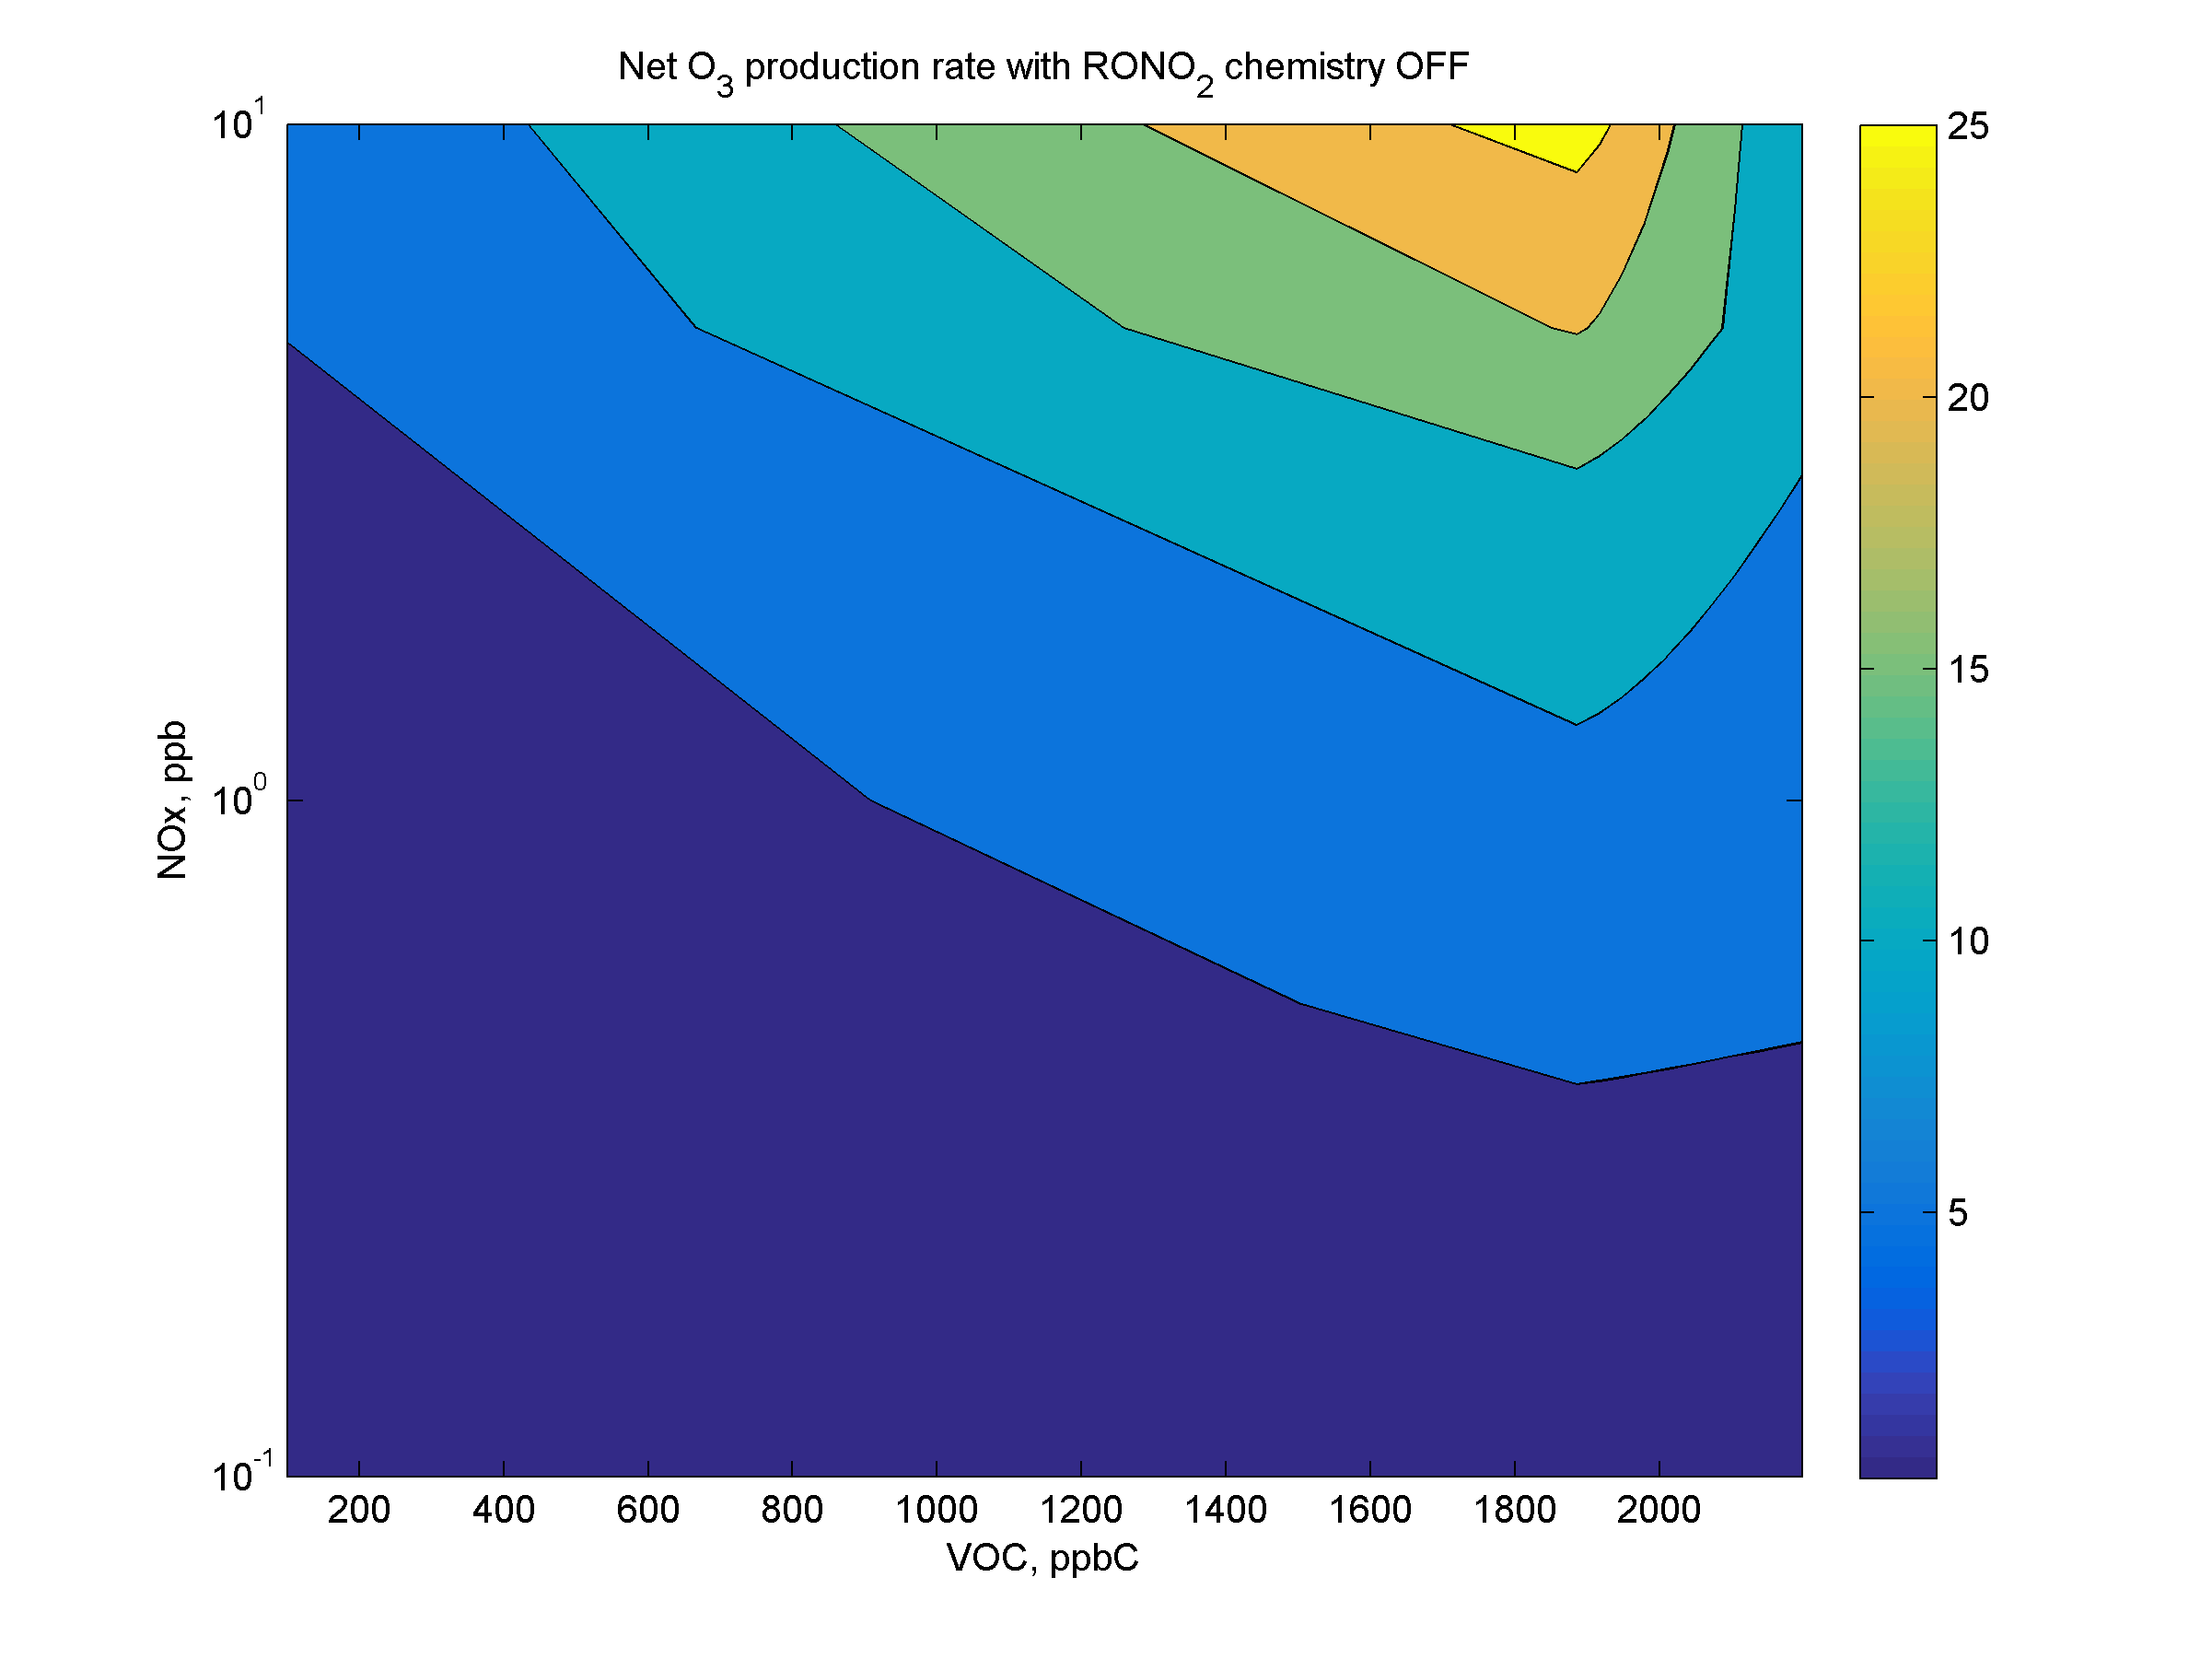
\includegraphics[width=.99\linewidth]{D:/FACSIMILE/ANsCBmodel/matlab/ANsCB_pics/ANsNOxVOC/noAN/chem_noAN_netO3rate_withINORG_NOx_1ppb_100ppb.png}
  \captionof{figure}{Isopleths giving net rate of $O_3$ production (ppb/h, color) as a function of $VOC$ (ppbC) and $NO_x$ (ppb) in the first modelling experiment with alkyl nitrate chemistry switched off combined with an additional run with inorganic chemistry only (i.e. the only $VOC$ is $CO$).}\label{fig:noAN_netO3rate}
\end{minipage}
\end{figure}
%%%%%%%%%%%%%%%%%%%%%%%%%%%%%%%%%%%%%%%%%%%%%%%%%%%%%%%%%%%%%%%%%%%%

Rewrite!

The same kind of plot can be found in Figure \ref{fig:noAN_netO3rate}, which is produced using data from our model from the first experiment with alkyl nitrate chemistry switched off. Taking into account the fact that the maximum $NO_x$ mixing ratio considered in the experiment is 10 ppb, our results are directly comparable only with a part of the data from Figure \ref{fig:Sillman1999}, namely with those inside the green dashed square. Moreover, since the minimum $NO_x$ mixing ratio considered in the experiment is 5 ppt, while the corresponding value in Figure \ref{fig:Sillman1999} is 1 ppb, a negative $O_3$ production rate is seen in our results, whereas it stays out of range of Figure \ref{fig:Sillman1999}.

One can see the same pattern in these two figures. At high $VOC$/$NO_x$ ratios, the rate of $O_3$ production increases with increasing $NO_x$ and reaches its maximum at the highest $NO_x$ and $VOC$ levels (which corresponds to the top right corner of the green dashed square). The change in $O_3$ production rate at high $VOC$/$NO_x$ ratios in our model is largely insensitive to $VOC$, which fits into the theory. At low $VOC$/$NO_x$ ratios the $O_3$ production rate starts to depend on $VOC$ concentration also resembling the behaviour of ozone isopleths at the top left corner of the green dashed square. The overall tendency of $O_3$ production rate to increase with increasing $VOC$ and $NO_x$ is present in both figures showing that the model reproduces this feature according to the theory. However, the modelled values of $O_3$ production rates are much lower than those in Figure \ref{fig:Sillman1999}: in the model the maximum production rate is 9 ppb/h, while in theory it is 30 ppb/h, meaning that our model underestimates the $O_3$ production rate, but reproduces some features of the relationship between $O_3$, $NO_x$ and $VOC$.

\section{Results} \label{sec:res}
\subsection{Sensitivity of $O_3$ production to alkyl nitrate chemistry}\label{sec:res_O3ANsensetivity}

To evaluate the sensitivity of $O_3$ production to alkyl nitrate chemistry under different $NO_x$ and $VOC$ conditions a number of simulations were carried out. In these simulations the chemical mechanism of the model was adjusted to either include or exclude the formation and loss of alkyl nitrates, which was accomplished by switching on and off all reactions that involve $RONO_2$ while keeping the rest of the mechanism unchanged. 

As it has been noted in Section \ref{sec:intro}, the relationship between $O_3$ and $RONO_2$ production rates is controlled by the branching ratio ($\alpha_3$) between reactions:
\begin{equation}\label{reac:RO2+NO=RO+NO2}
RO_2 + NO \xrightarrow{1-\alpha_3} RO + NO_2
\end{equation}
\begin{equation}\label{reac:RO2+NO=RONO2}
RO_2 + NO \xrightarrow{\alpha_3} RONO_2
\end{equation}
Reaction (\ref{reac:RO2+NO=RO+NO2}) leads to $O_3$ production and $NO$ regeneration, resulting in continuing $O_3$ production, while reaction (\ref{reac:RO2+NO=RONO2}) terminates this process. Branching ratios used in the model are taken from the MCM v3.3, and their values (Table \ref{tab:ANbranching}) were kept constant in all model runs.
%%%%%%%%%%%%%%%%%%%%%%%%%%%%%%%%%%%%%%%%%%%%%%%%%%%%%%%%%%%%%%%%%%%%
\begin{table} %  AN branching ratios
\caption{Branching ratios for the formation of alkyl nitrates from their precursor peroxy radicals and $NO$ (taken from the MCM v3.3 (2015)).}\label{tab:ANbranching}
\centering
\begin{tabular}{cc}
\hline
Alkyl nitrate    & Branching ratio \\
\hline
methyl           & 0.001 \\
ethyl            & 0.009 \\
iso-propyl       & 0.042 \\
n-propyl         & 0.020 \\
n-butyl          & 0.033 \\
sec-butyl        & 0.090 \\
iso-butyl        & 0.033 \\ 
tert-butyl       & 0.025 \\
n-pentyl         & 0.052 \\
2-pentyl         & 0.129 \\
3-pentyl         & 0.131 \\
2-methylbutyl    & 0.052 \\
3-methyl-2-butyl & 0.141 \\
2-methyl-2-butyl & 0.047 \\
\hline
\end{tabular}
\end{table}
%%%%%%%%%%%%%%%%%%%%%%%%%%%%%%%%%%%%%%%%%%%%%%%%%%%%%%%%%%%%%%%%%%%%

Figure \ref{fig:netO3rate_noAN_withAN_diff} shows isopleths of net $O_3$ production rate as a function of $NO_x$ and sum of $VOCs$ initial concentrations from two series of model runs (with and without alkyl chemistry) and the difference between them. Since the actual formation of $O_3$ in our model starts at 250 ppt of $NO_x$, Figure \ref{fig:netO3rate_noAN_withAN_diff} summarises modelling data from experiments with $NO_x$ initial mixing ratios from 250 ppt till 100 ppb.

%%%%%%%%%%%%%%%%%%%%%%%%%%%%%%%%%%%%%%%%%%%%%%%%%%%%%%%%%%%%%%%%%%%%
\begin{figure} % netO3rate noAN withAN diff
\centering
\begin{minipage}{.3\textwidth}
  \centering
  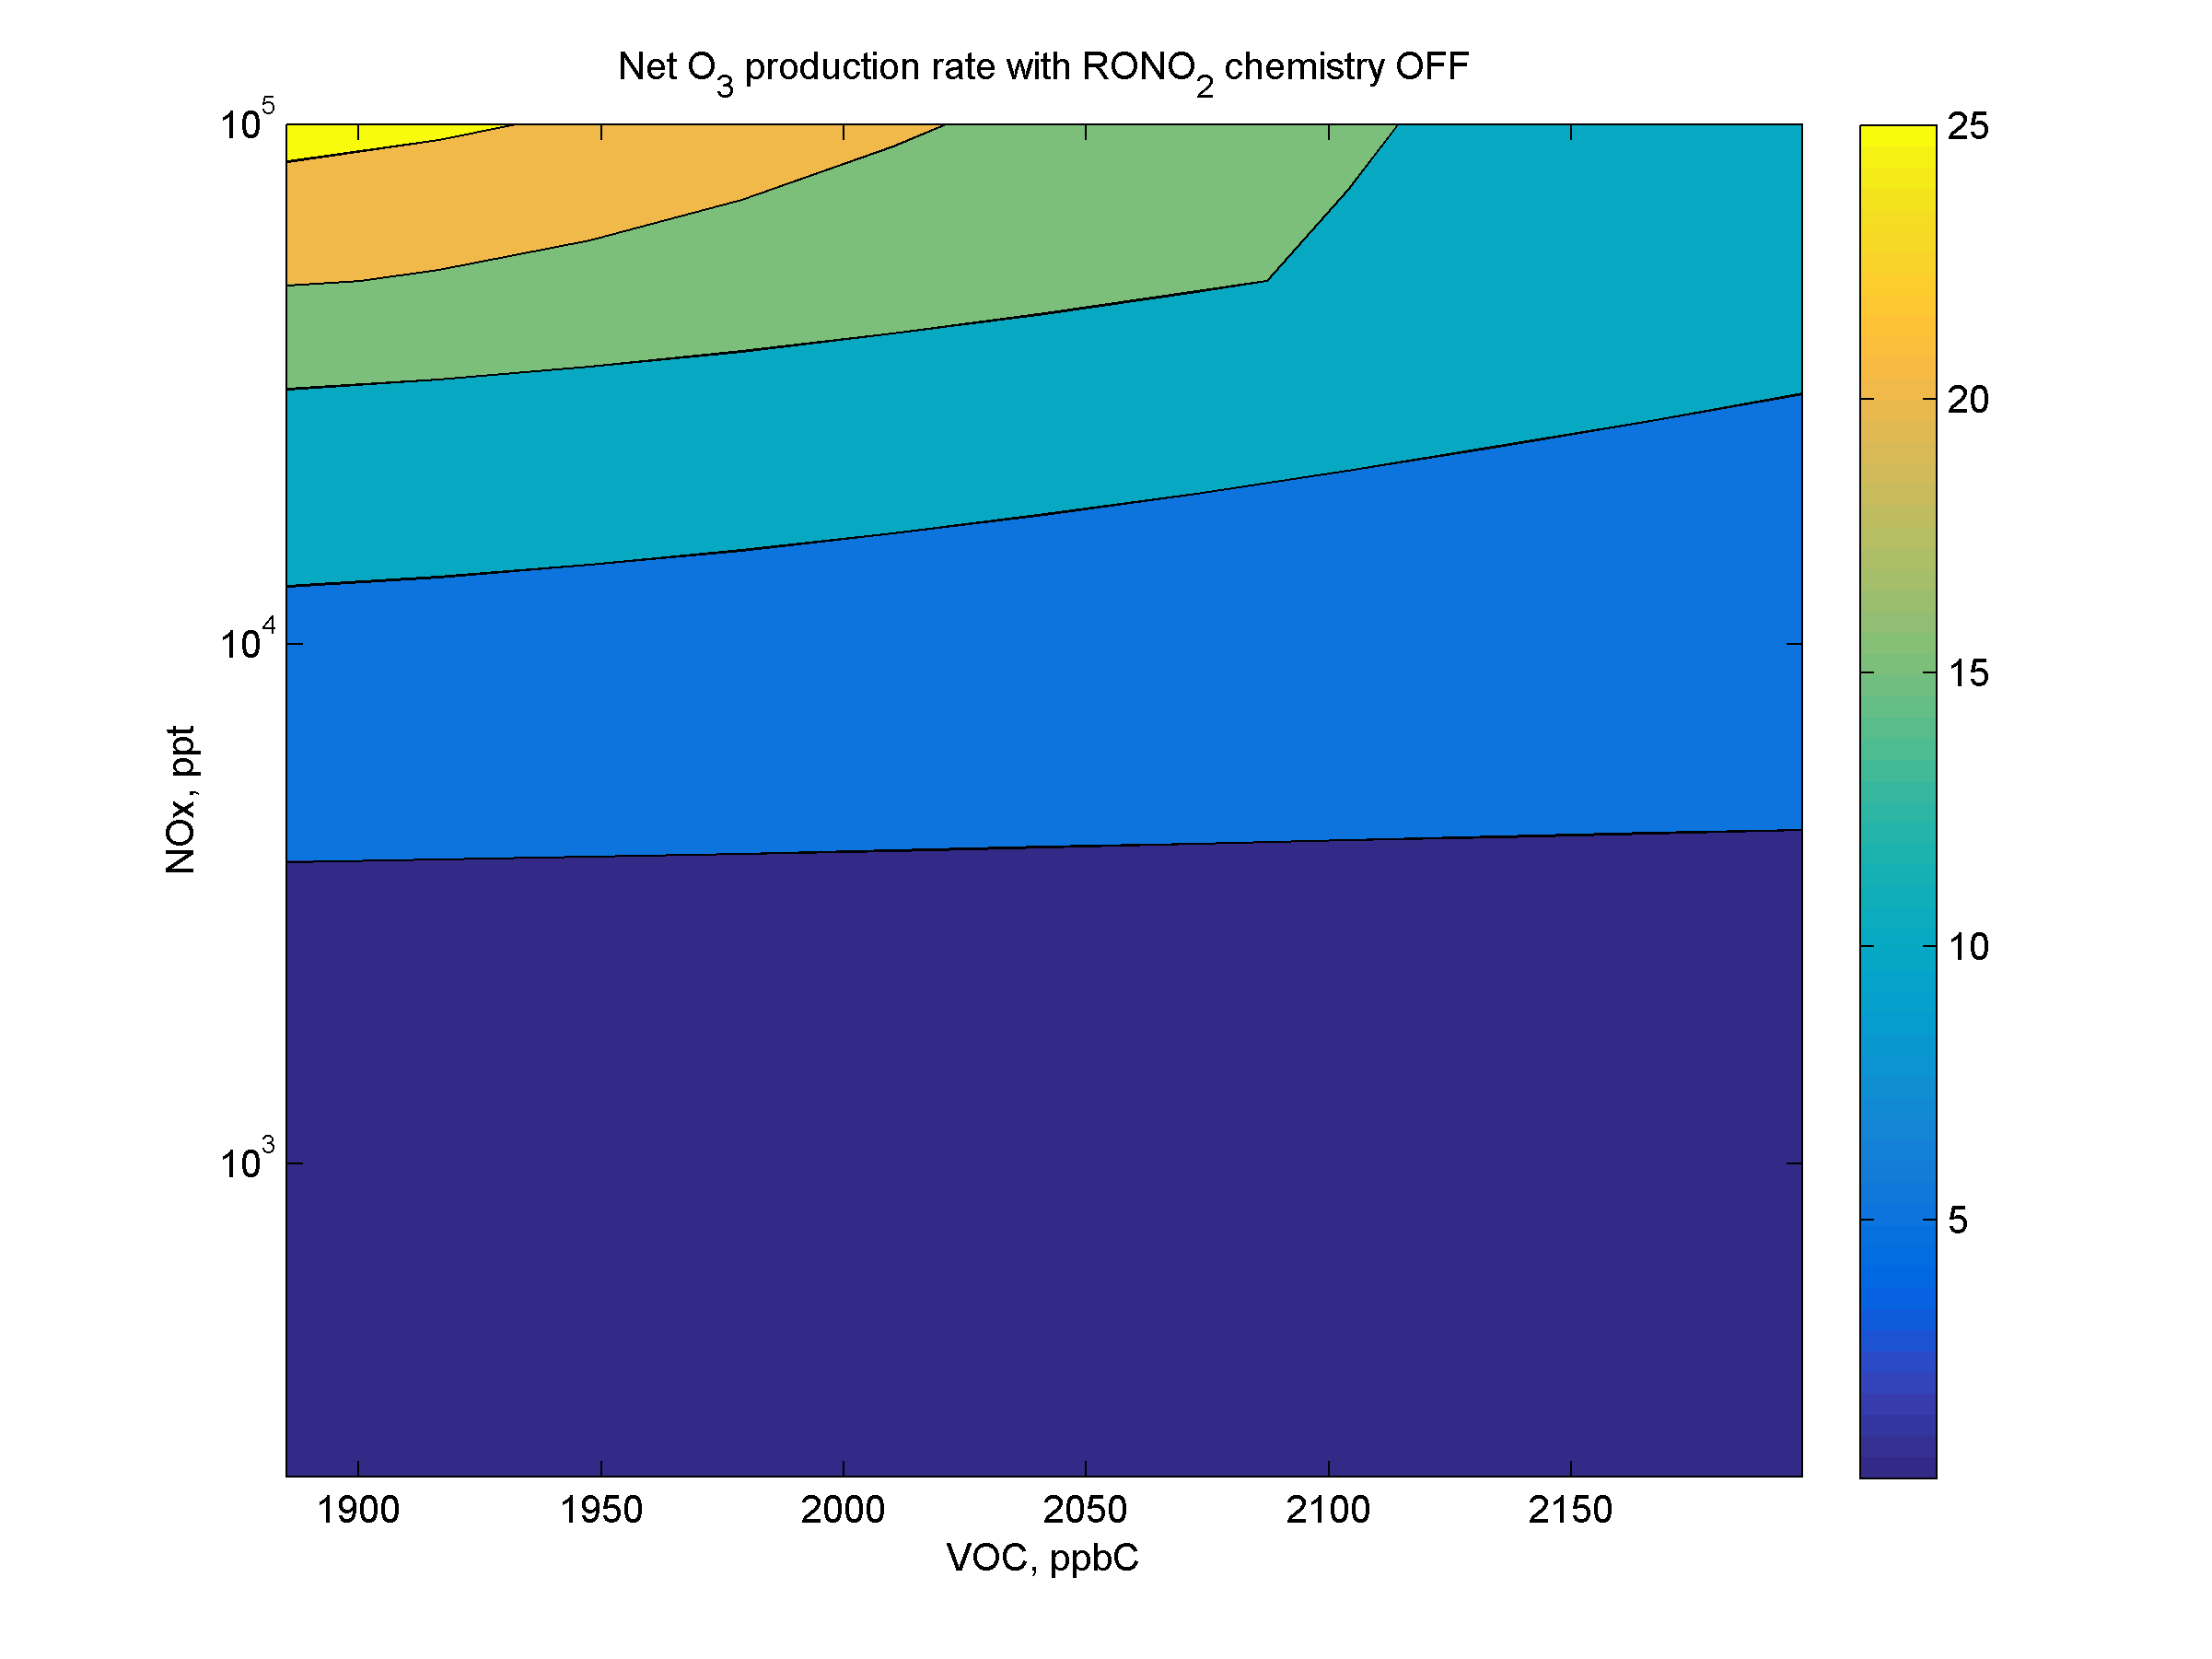
\includegraphics[width=.99\linewidth]{D:/FACSIMILE/ANsCBmodel/matlab/ANsCB_pics/ANsNOxVOC/noAN/chem_noAN_netO3rate_noINORG_NOx_250ppt_100ppb.png}
\end{minipage}
\begin{minipage}{.3\textwidth}
  \centering
  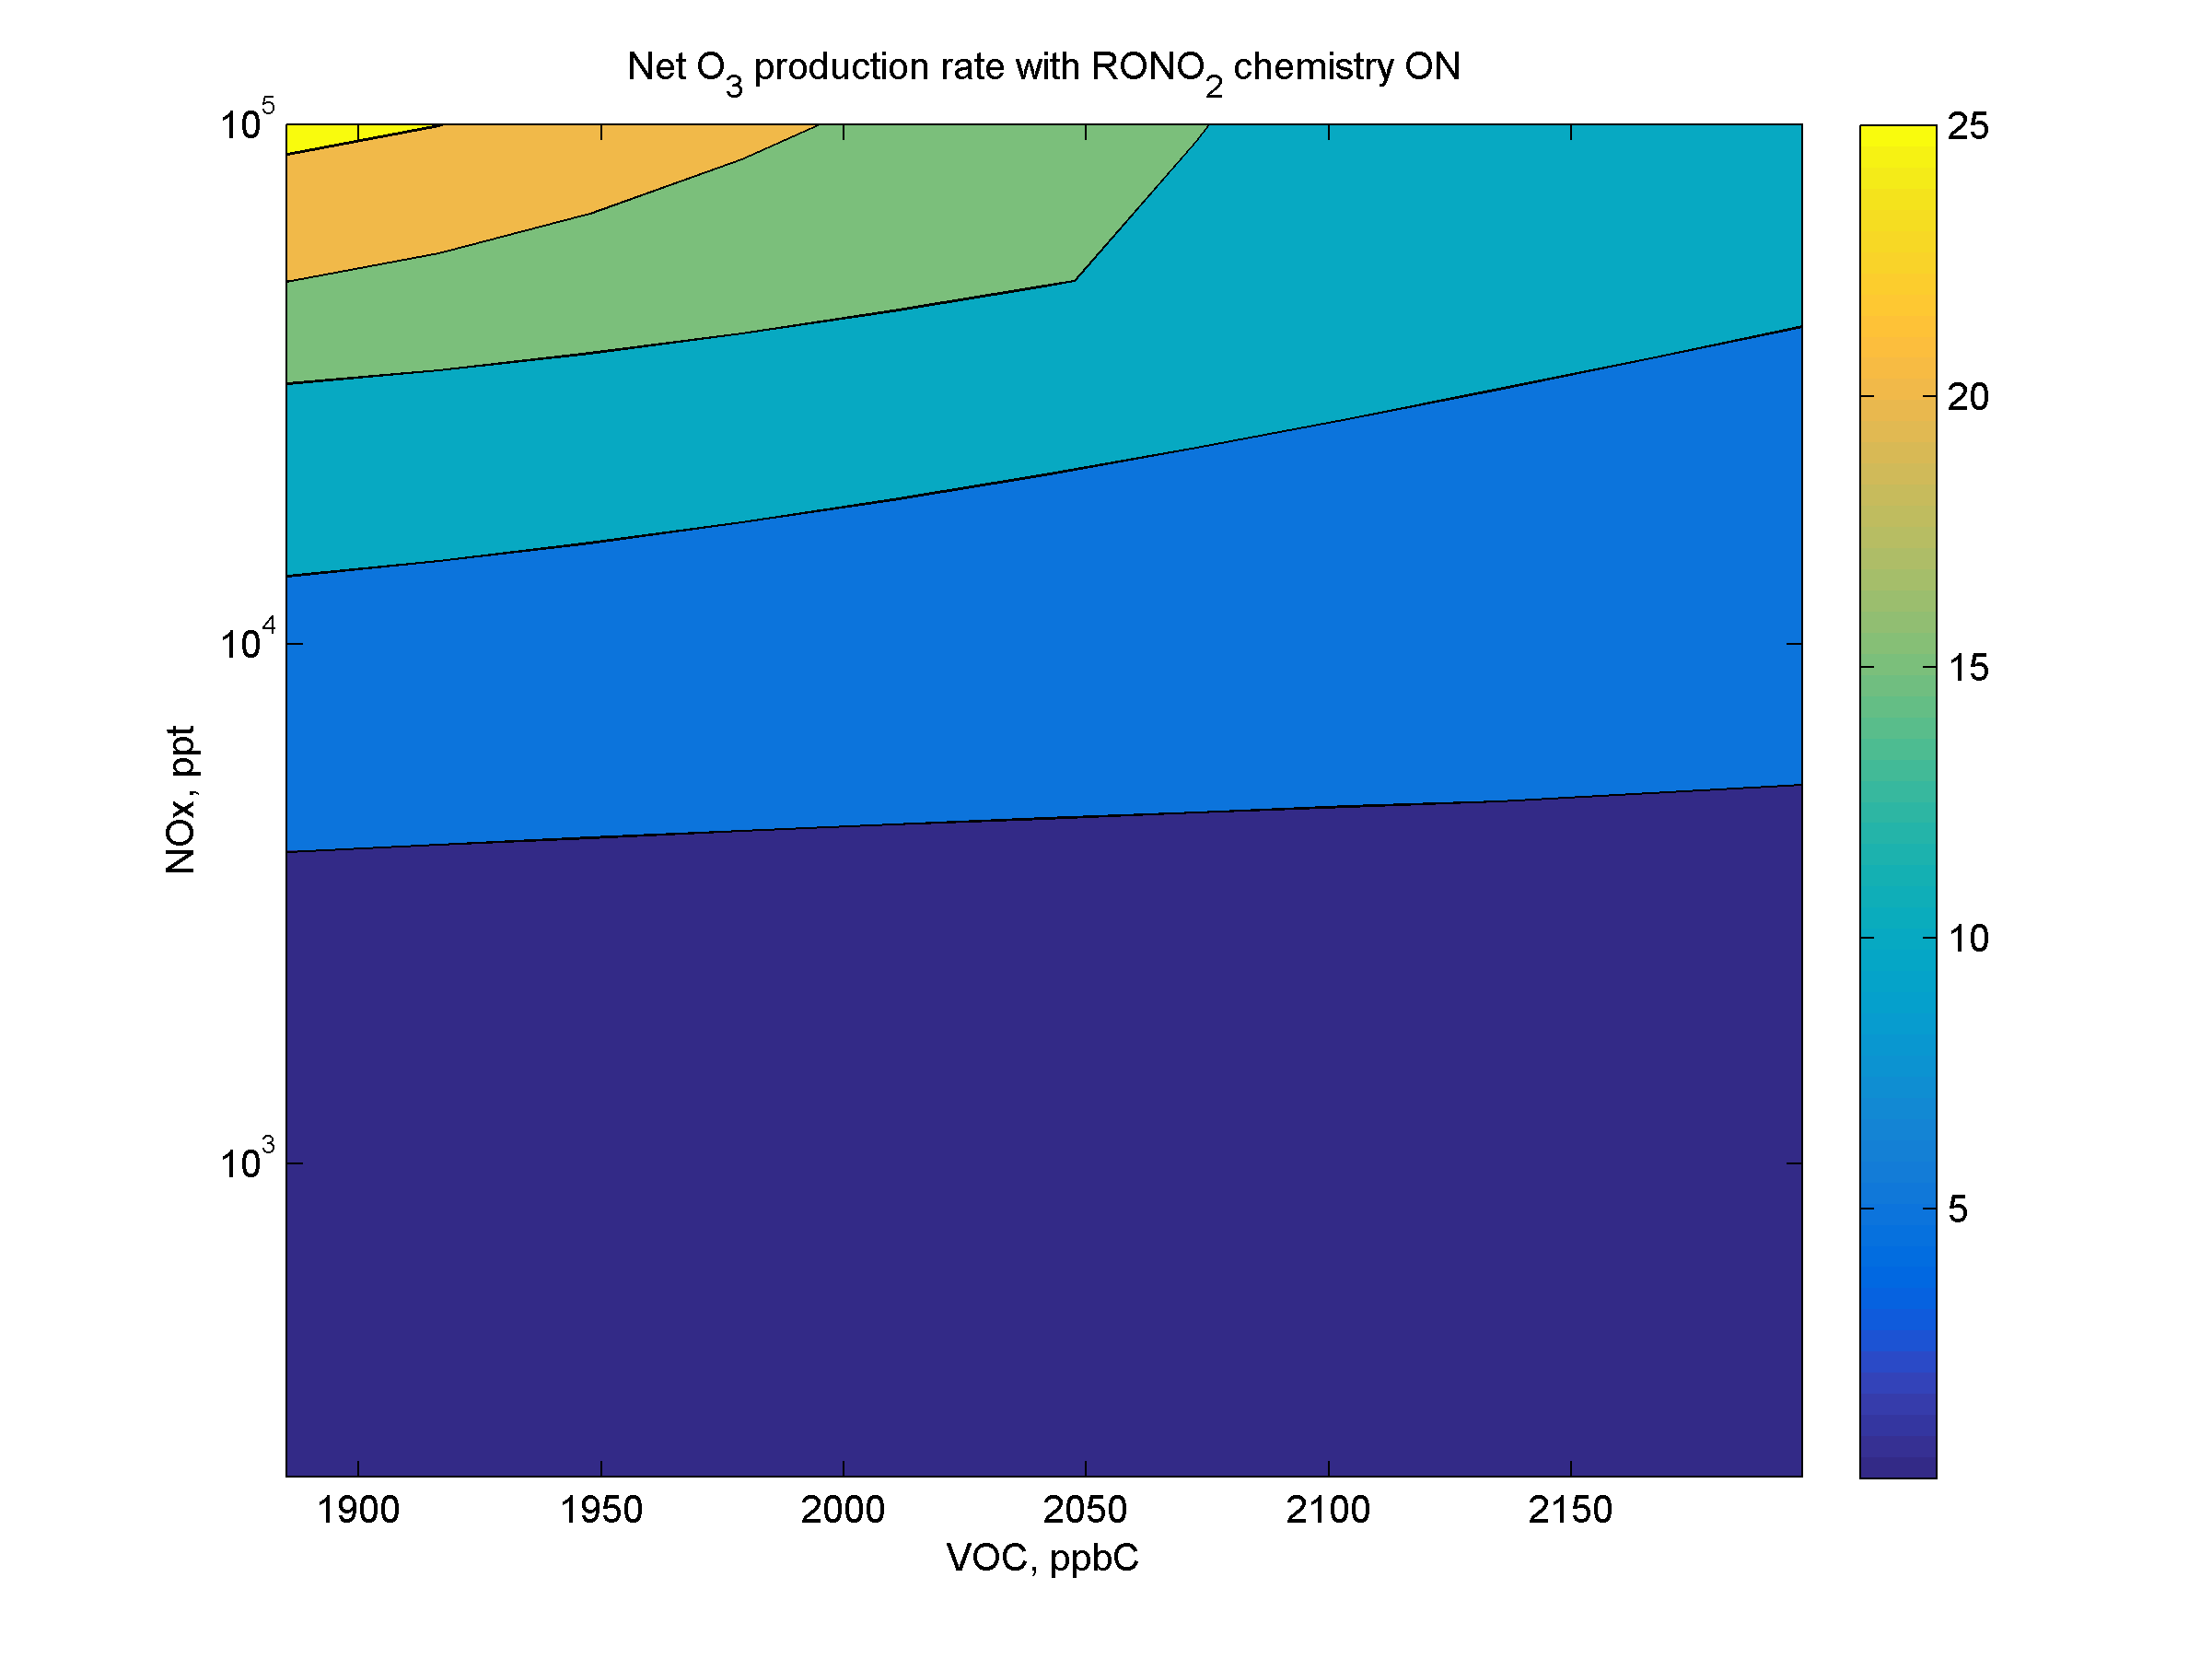
\includegraphics[width=.99\linewidth]{D:/FACSIMILE/ANsCBmodel/matlab/ANsCB_pics/ANsNOxVOC/allAN/chem_allAN_netO3rate_noINORG_NOx_250ppt_100ppb.png}
\end{minipage}
\begin{minipage}{.3\textwidth}
  \centering
  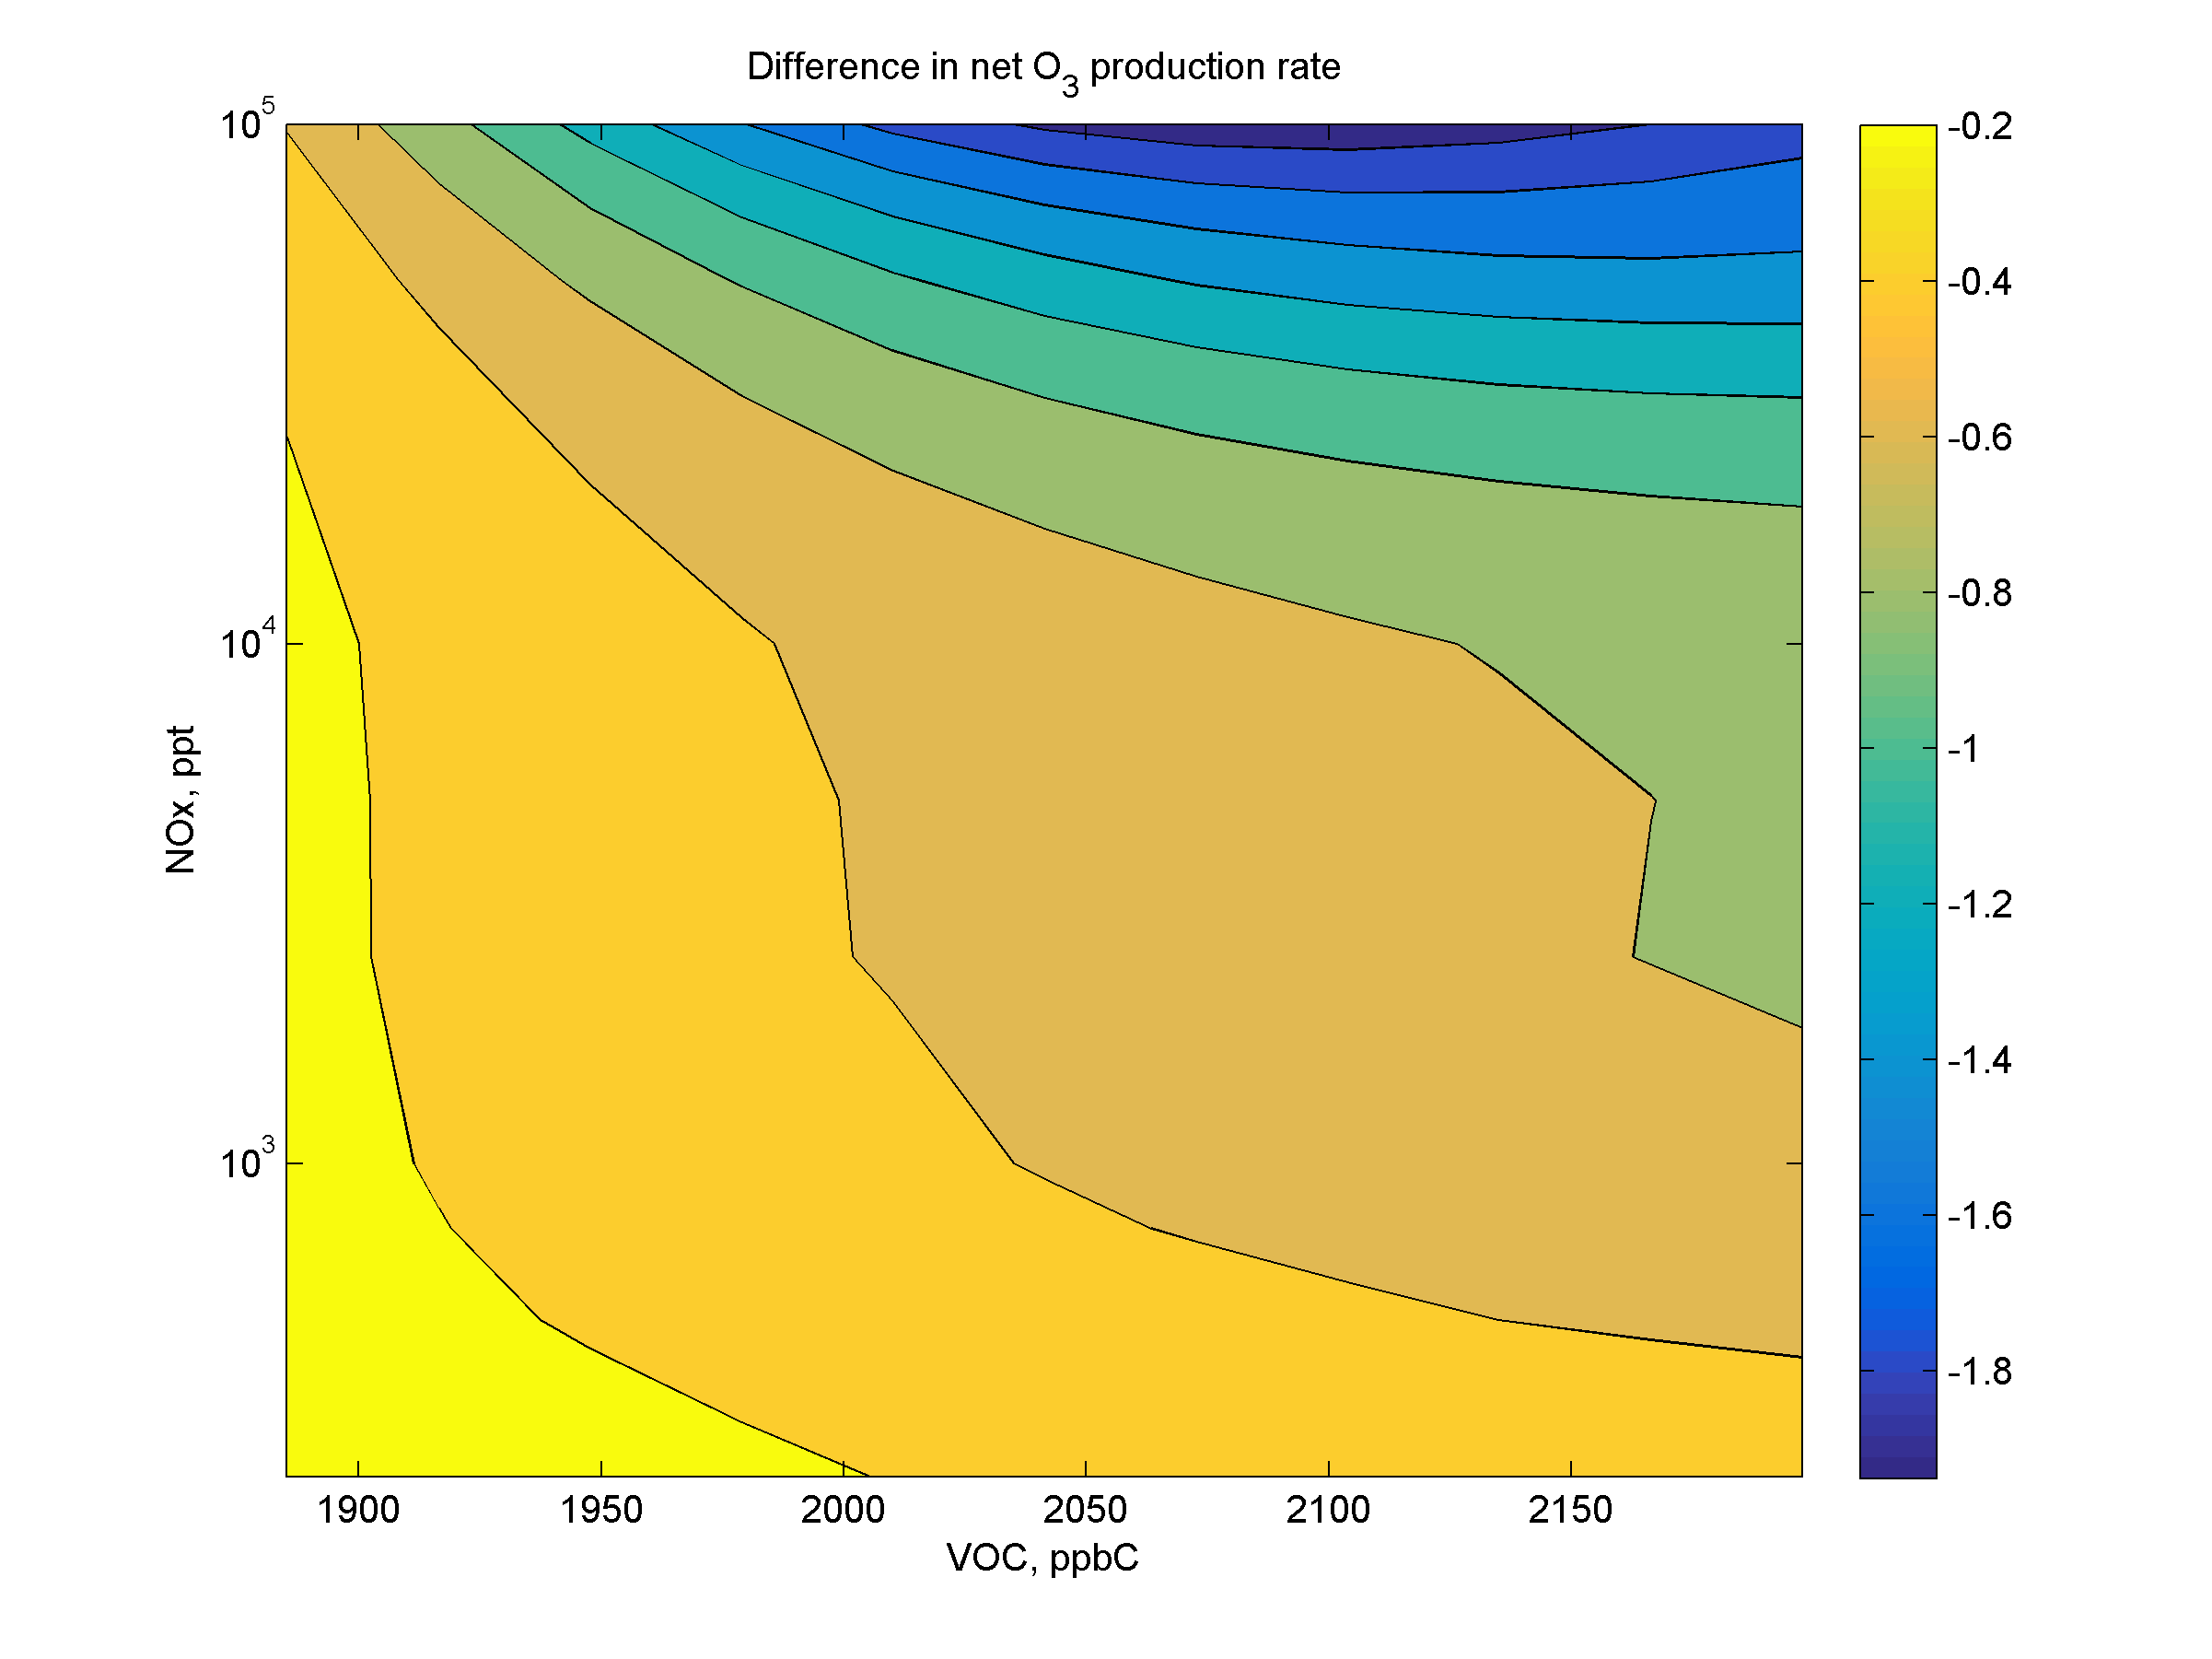
\includegraphics[width=.99\linewidth]{D:/FACSIMILE/ANsCBmodel/matlab/ANsCB_pics/ANsNOxVOC/allAN/chem_allAN_netO3ratediff_noINORG_NOx_250ppt_100ppb.png}
\end{minipage}
\caption{Isopleths giving net rate of $O_3$ production (ppb/h, color) as a function of $VOC$ (ppbC) and $NO_x$ (ppb) with alkyl nitrate chemistry switched off (left) and switched on (middle). Difference between them is shown on the right.}\label{fig:netO3rate_noAN_withAN_diff}
\end{figure}
%%%%%%%%%%%%%%%%%%%%%%%%%%%%%%%%%%%%%%%%%%%%%%%%%%%%%%%%%%%%%%%%%%%%

As expected, the inclusion of alkyl nitrate chemistry slows down the net $O_3$ production rate. At low $NO_x$ and $VOCs$ initial levels, this slowdown is -0.2...-0.6 ppb of $O_3$ per hour. As $NO_x$ and $VOCs$ levels increase the $O_3$ production rate decreases, reaching the maximum decrease of -1.94 ppb of $O_3$ per hour at 100 ppb of $NO_x$ and $VOCs$ level from case I (not the highest $VOCs$ level). At the range of $NO_x$ levels from 1 ppb to 10 ppb the difference in $O_3$ production rate is slightly more sensitive to $VOCs$ levels, while it is almost insensitive to $VOCs$ at $NO_x$ levels higher than 10 ppb and 2050 ppbC of $VOCs$. 
%%%%%%%%%%%%%%%%%%%%%%%%%%%%%%%%%%%%%%%%%%%%%%%%%%%%%%%%%%%%%%%%%%%%%
\begin{figure} % netO3mixrat noAN allAN diff diffpercent
\centering
\begin{minipage}{.4\textwidth} % noAN
  \centering
  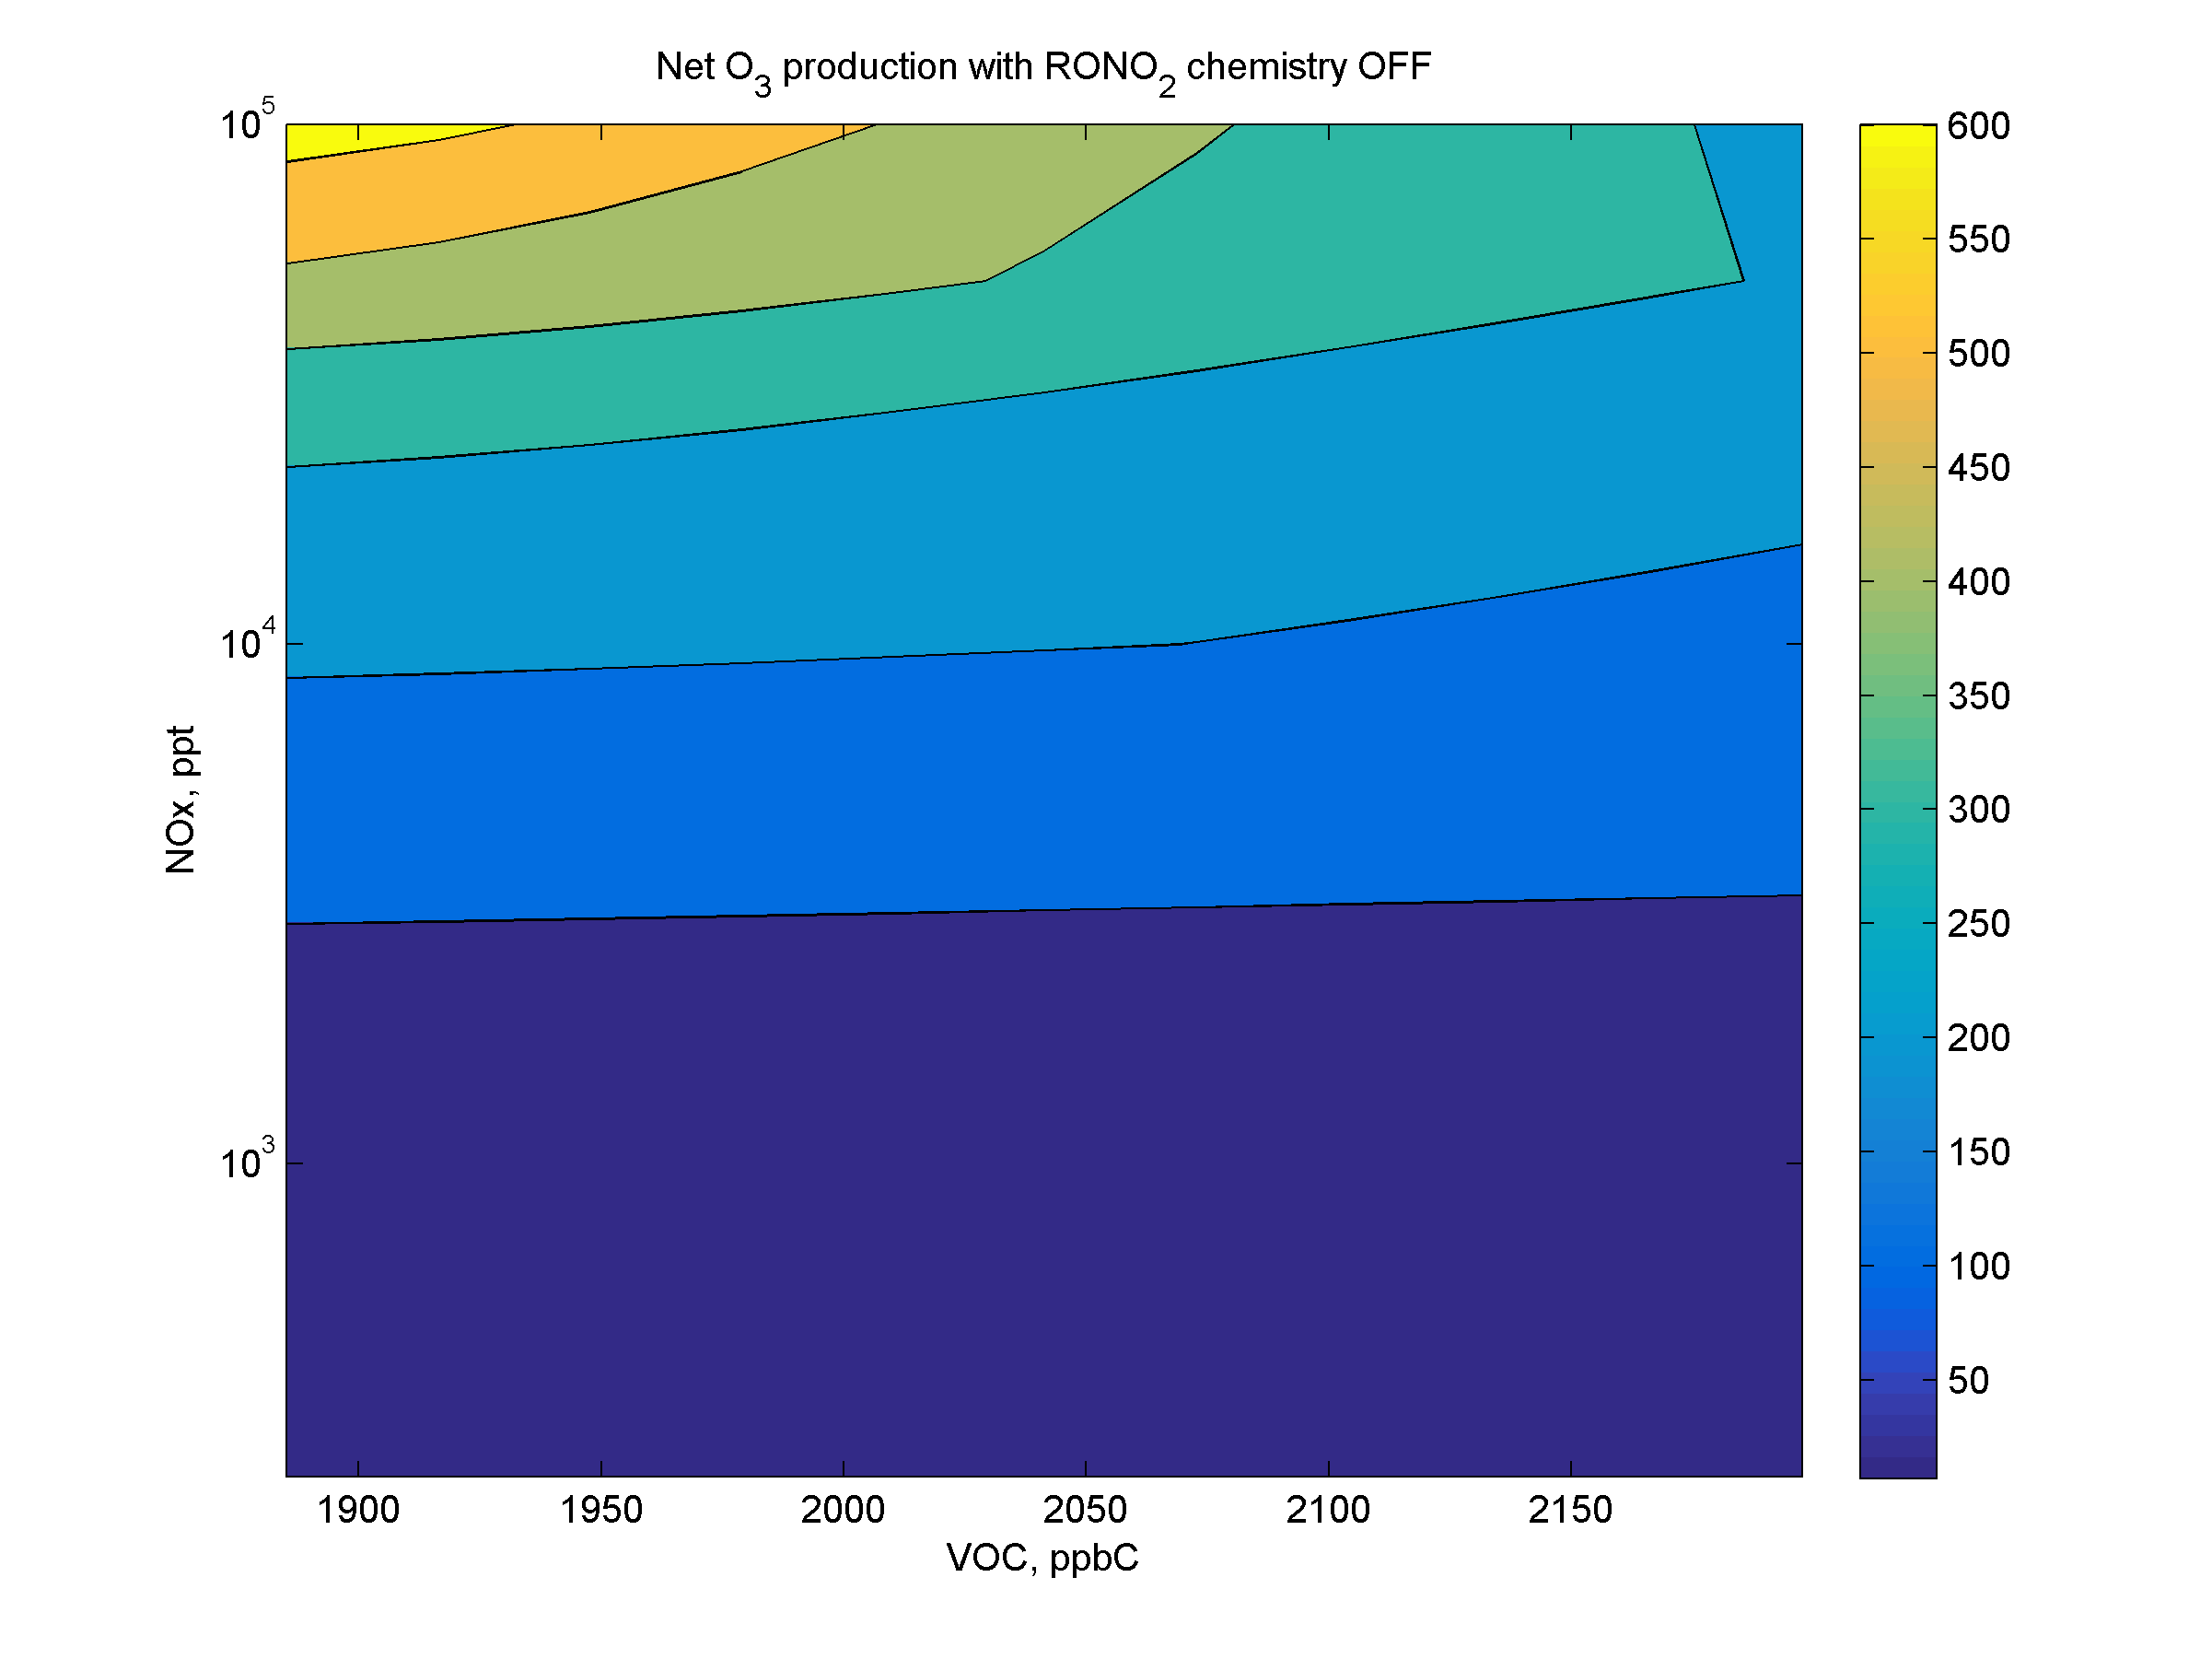
\includegraphics[width=.99\linewidth]{D:/FACSIMILE/ANsCBmodel/matlab/ANsCB_pics/ANsNOxVOC/noAN/chem_noAN_netO3mixrat_noINORG_NOx_250ppt_100ppb.png}
\end{minipage}
\begin{minipage}{.4\textwidth} % diff
  \centering
  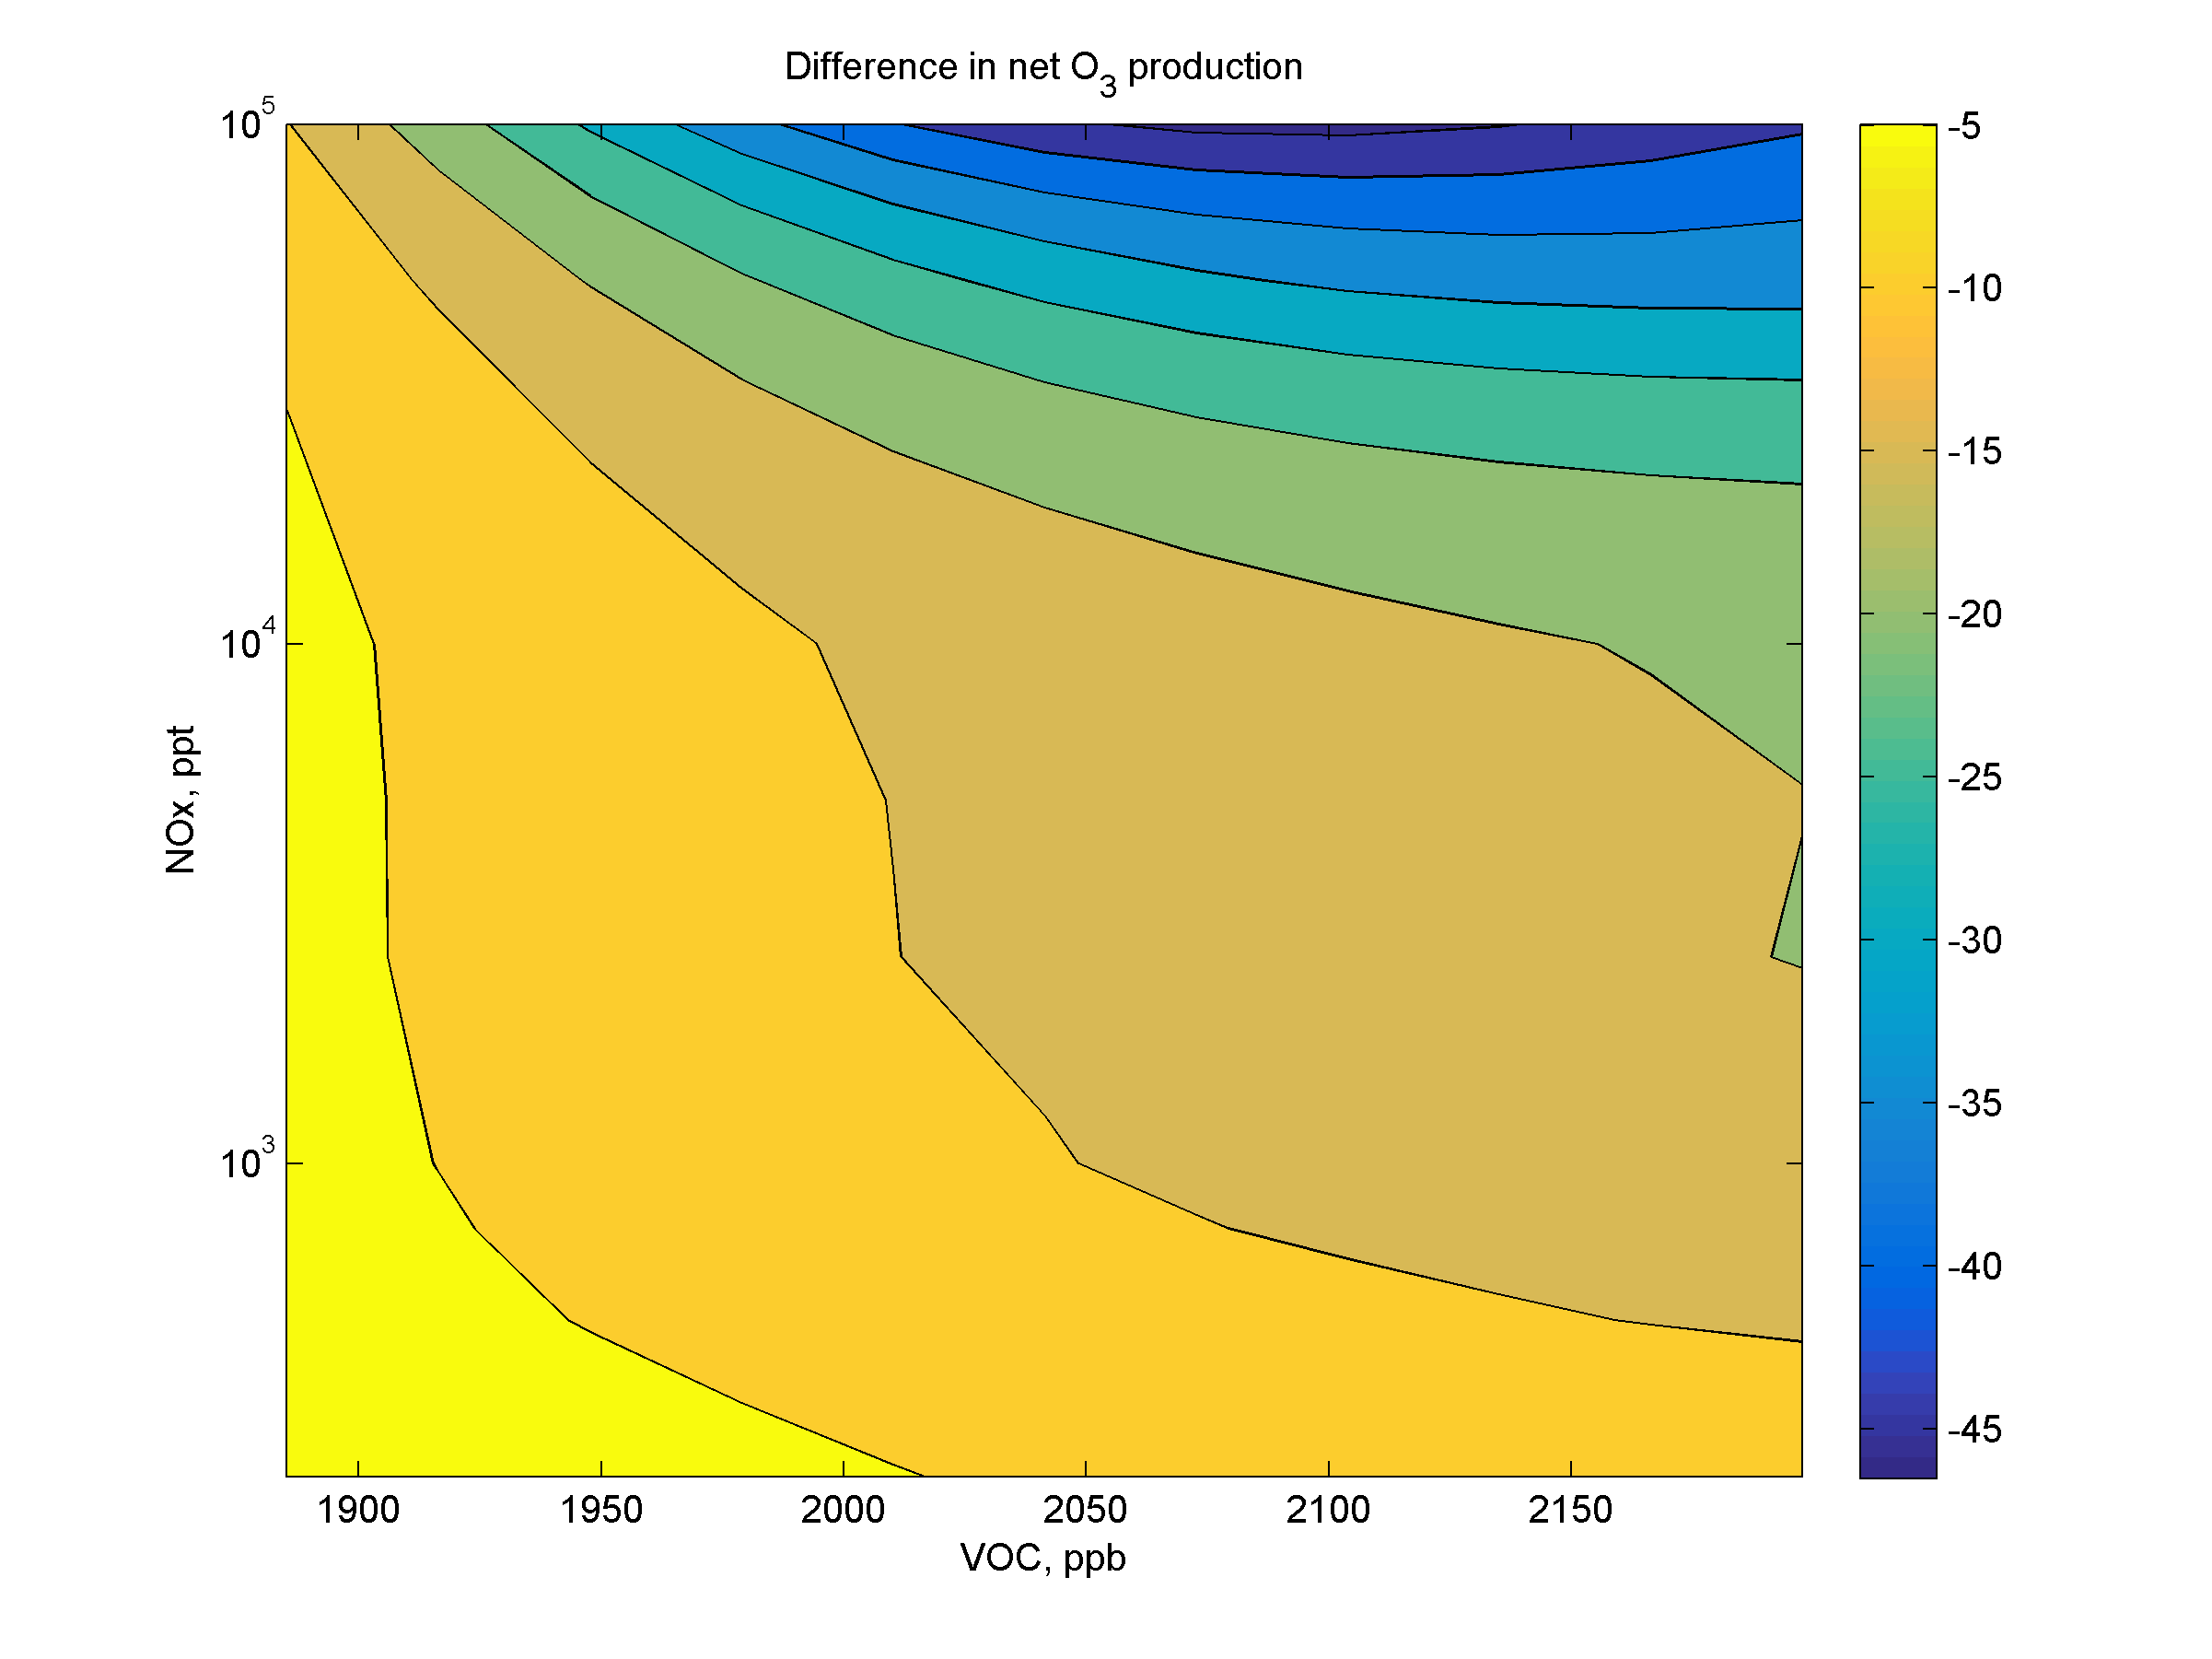
\includegraphics[width=.99\linewidth]{D:/FACSIMILE/ANsCBmodel/matlab/ANsCB_pics/ANsNOxVOC/allAN/chem_allAN_netO3mixratdiff_noINORG_NOx_250ppt_100ppb.png}
\end{minipage}
\begin{minipage}{.4\textwidth} % allAN
  \centering
  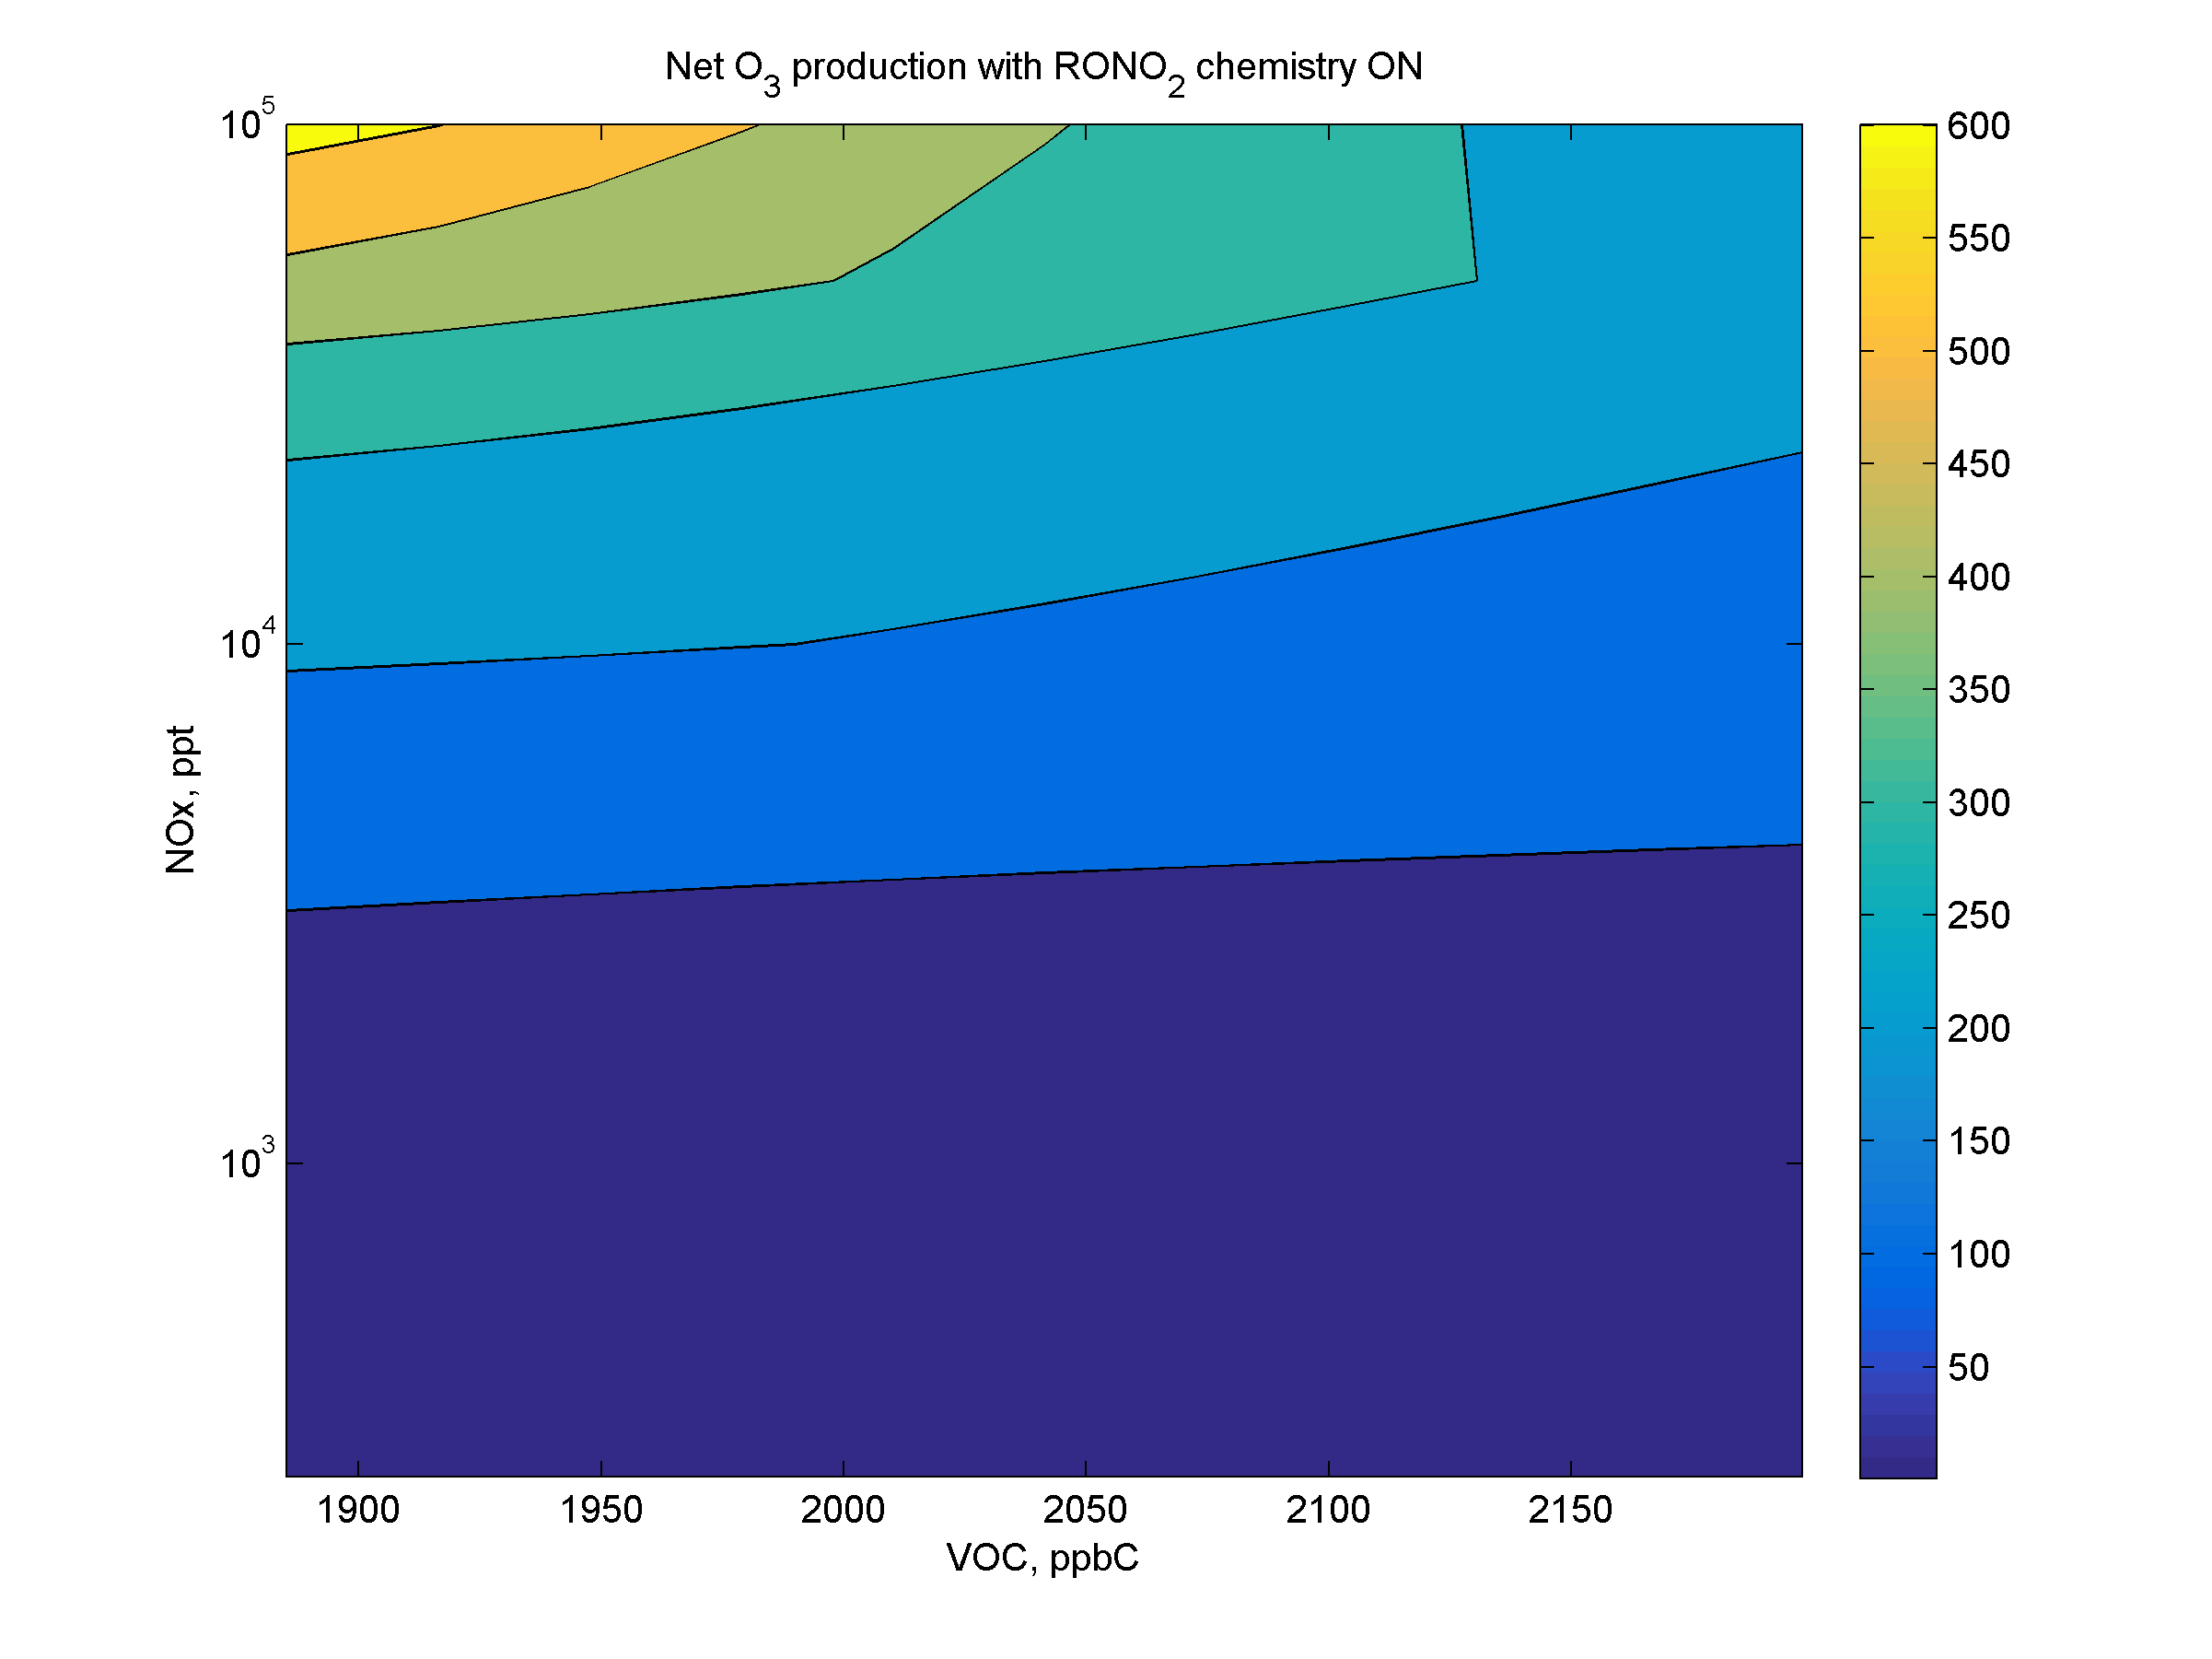
\includegraphics[width=.99\linewidth]{D:/FACSIMILE/ANsCBmodel/matlab/ANsCB_pics/ANsNOxVOC/allAN/chem_allAN_netO3mixrat_noINORG_NOx_250ppt_100ppb.png}
\end{minipage}
\begin{minipage}{.4\textwidth} % diffpercent
  \centering
  \includegraphics[width=.99\linewidth]{D:/FACSIMILE/ANsCBmodel/matlab/ANsCB_pics/ANsNOxVOC/allAN/chem_allAN_netO3mixratdiffpercent_noINORG_NOx_250ppt_100ppb.png}
\end{minipage}
\caption{Isopleths giving net $O_3$ production (ppb, color) as a function of $VOC$ (ppbC) and $NO_x$ (ppb, range 250 ppt - 100 ppb) with alkyl nitrate chemistry switched off (a) and switched on (b). Absolute difference (with alkyl nitrates minus without them) between two series of model runs in ppb (c), same in \% (d). Net production = final - initial value of $O_3$ mixing ratio.}\label{fig:netO3mixrat_noAN_withAN_diff}
\end{figure}
%%%%%%%%%%%%%%%%%%%%%%%%%%%%%%%%%%%%%%%%%%%%%%%%%%%%%%%%%%%%%%%%%%%%%

The change in net rate of $O_3$ production due to inclusion of alkyl nitrate chemistry into the chemical mechanism has a direct impact on absolute $O_3$ levels calculated by the model. Figure \ref{fig:netO3mixrat_noAN_withAN_diff} shows that the net $O_3$ production (difference between final and initial $O_3$ mixing ratio) is smaller when alkyl nitrate chemistry is switched on. At low $NO_x$ and $VOCs$ levels the negative (!) change in the net $O_3$ production is 5-10 ppb, at high $NO_x$ and $VOCs$ levels it is 35-45 ppb (per 24 hours) with maximum value of 46.5 ppb.

These changes in the net $O_3$ production should be treated with care, because the model due to reasons described in Section \ref{sec:method} gives unrealistically high $O_3$ mixing ratios. The maximum $O_3$ mixing ratio in the model is equal to 650 ppb (at the highest $NO_x$ level (100 ppb) and the lowest $VOCs$ level (case A)), while maximum typical urban (Los Angeles, Mexico City) $O_3$ mixing ratio is 490 ppb (http://www-personal.umich.edu/~sillman/ozone.htm). Therefore, a more useful estimate is a percentage difference in $O_3$ mixing ratios between two series of model runs shown in Figure \ref{fig:netO3rate_noAN_withAN_diff} DDDDD!. It appears that the largest absolute changes in $O_3$ mixing ratios (40-45 ppb) are changes by only 20-30\%, while changes up to 90\% take place the model is in low $NO_x$ and high $VOCs$ conditions.

To see what caused these changes it is useful to look at the net production of the sum of the alkyl nitrates themselves as a function of $NO_x$ (250 ppt - 100 ppb) and $VOCs$ (Figure \ref{fig:endtotalANs}). Since alkyl nitrates are the only sink for $NO_x$ in our model high production of these species was expected. The $NO_x$-$VOC$ field of total $RONO_2$ isopleths is mostly characterized by mixing ratios of ppb level (0.2-1.4 ppb), while the observations show that their mean mixing ratios lay at a level of tens-thousands of ppt (Table \ref{tab:ANmean}). Nevertheless, Figure \ref{fig:endtotalANs} will be of interest to other researches, because it is probably the first ever attempt to derive the distribution of $\Sigma RONO_2$ mixing ratios in $NO_x$-$VOC$ field.

%%%%%%%%%%%%%%%%%%%%%%%%%%%%%%%%%%%%%%%%%%%%%%%%%%%%%%%%%%%%%%%%%%%%%
\begin{figure} % endtotalANs
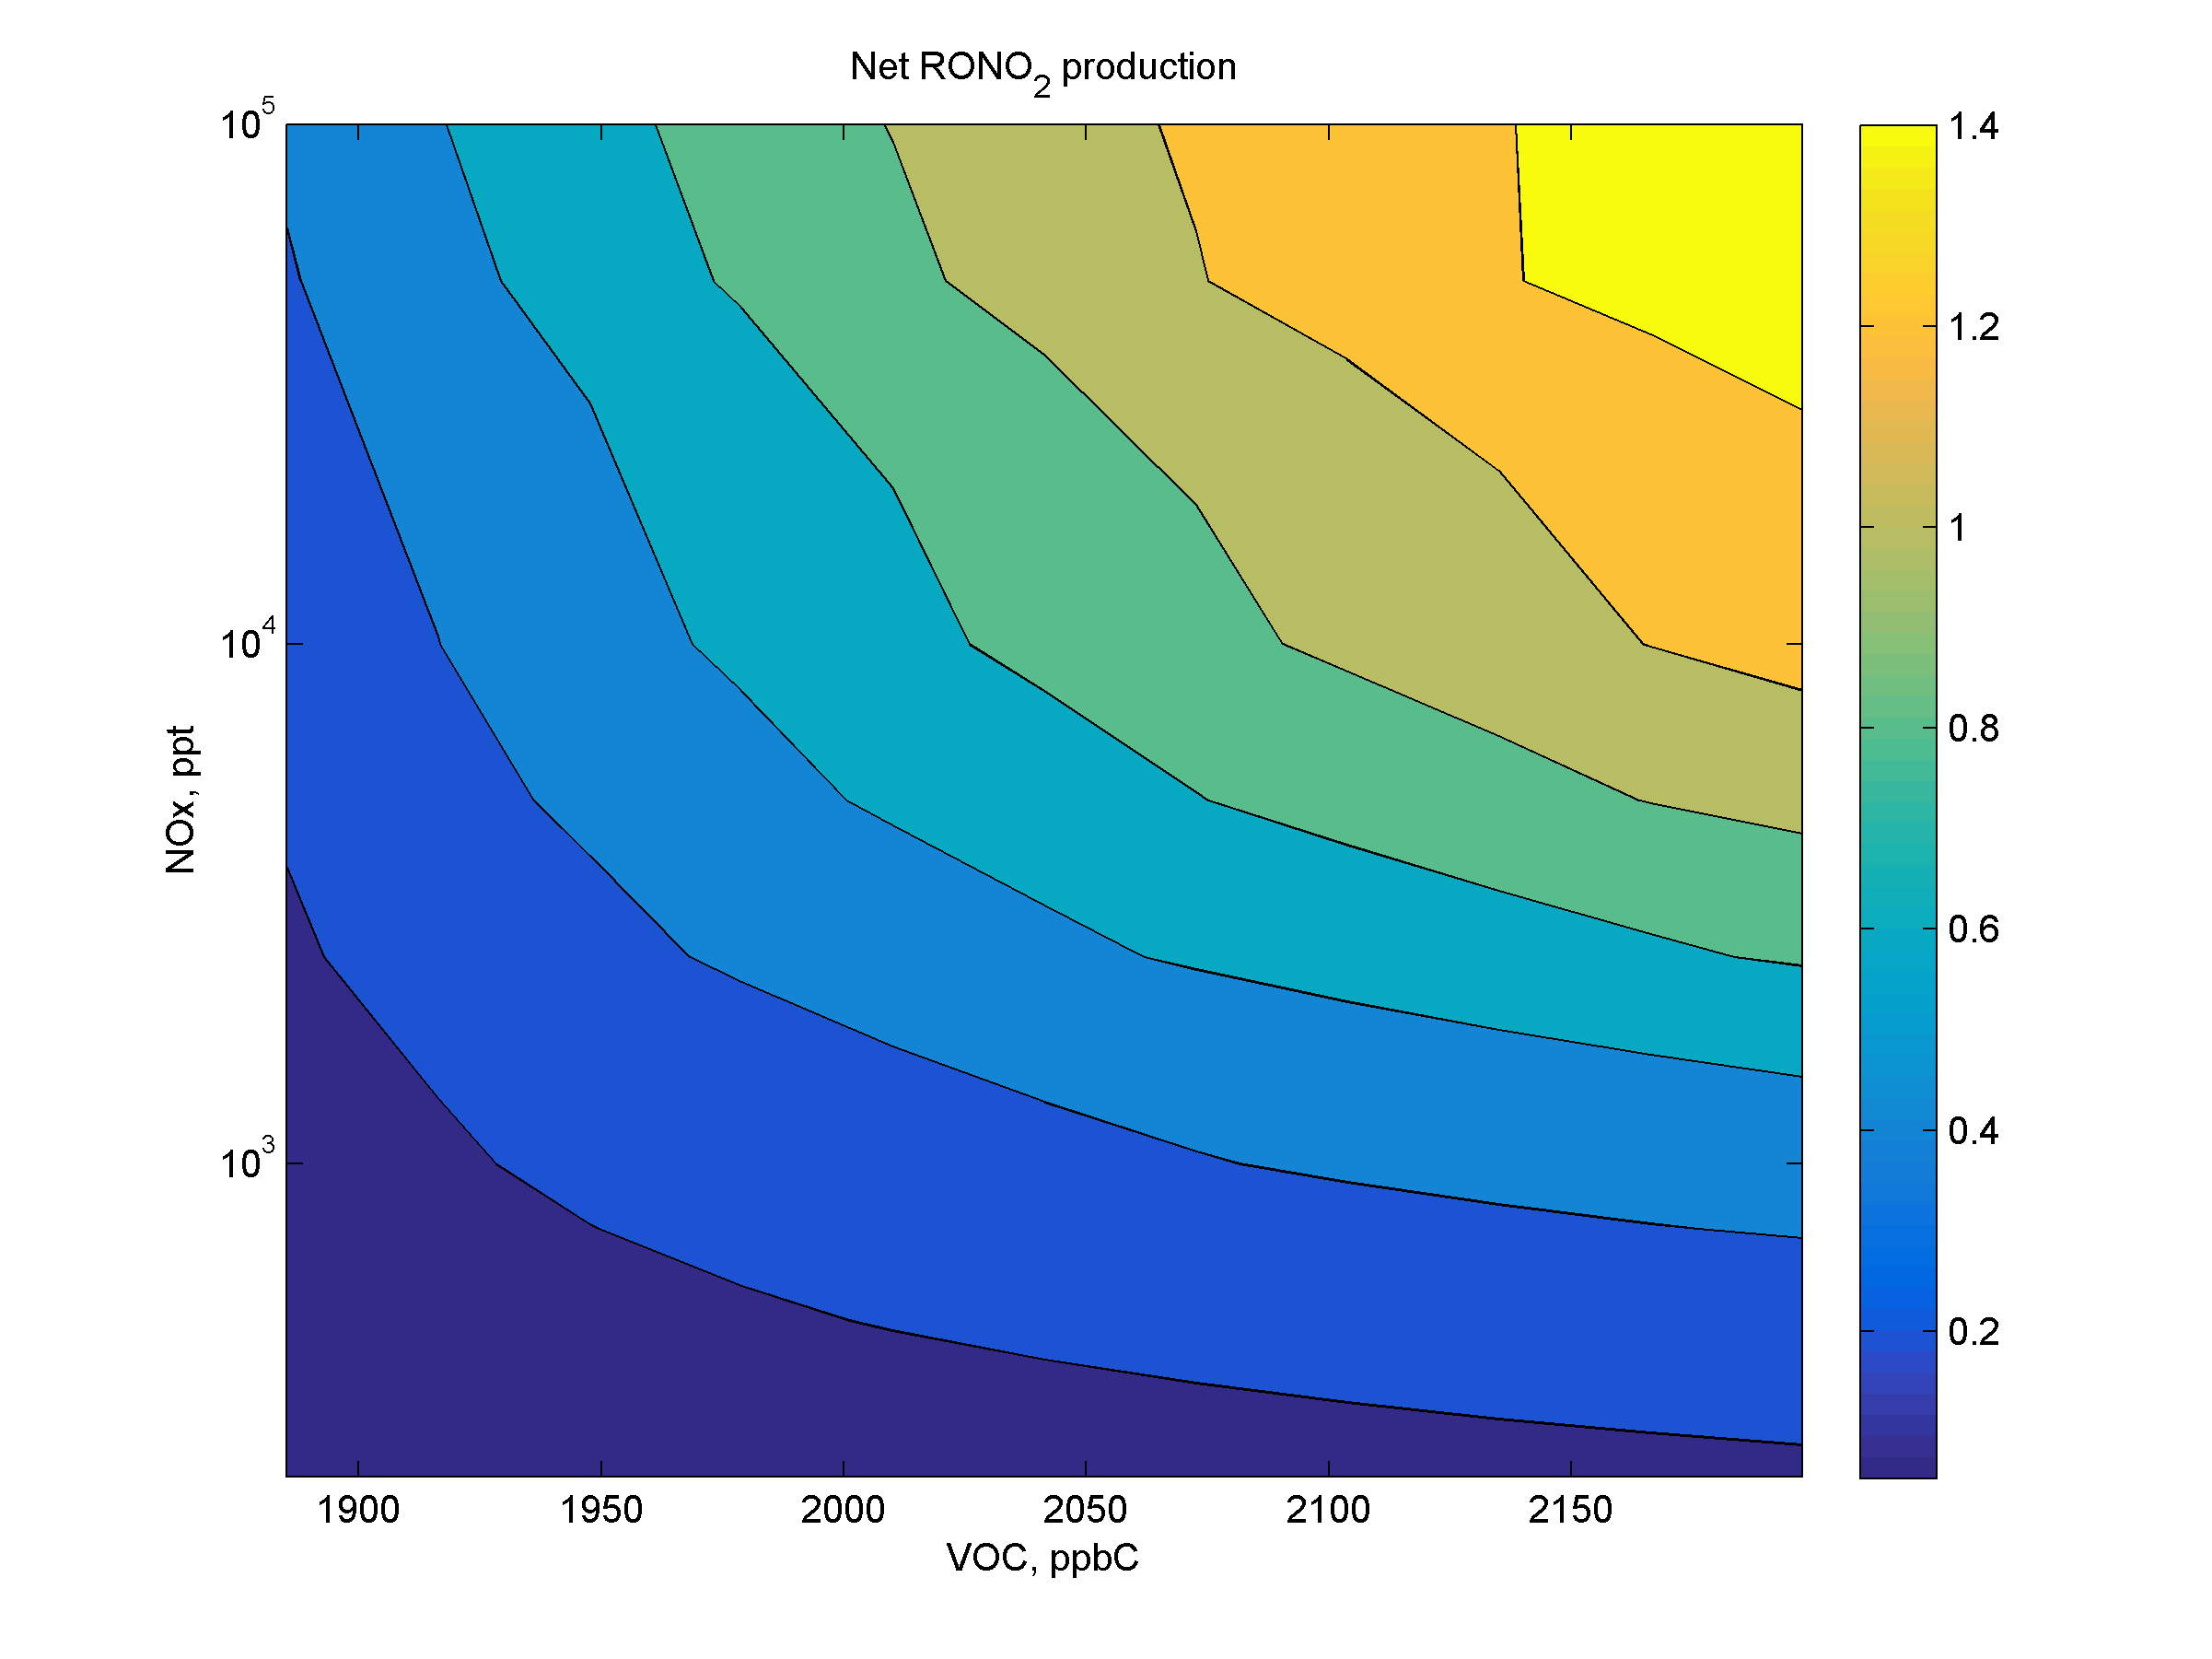
\includegraphics[width=.5\linewidth]{D:/FACSIMILE/ANsCBmodel/matlab/ANsCB_pics/ANsNOxVOC/allAN/chem_allAN_endtotalANs_noINORG_NOx_250ppt_100ppb.png}
\caption{Isopleths of net production of alkyl nitrates ($\Sigma RONO_2$) as a function of $NO_x$ and $VOCs$ levels.}\label{fig:endtotalANs}
\end{figure}
%%%%%%%%%%%%%%%%%%%%%%%%%%%%%%%%%%%%%%%%%%%%%%%%%%%%%%%%%%%%%%%%%%%%%
! Dependence of alkyl nitrate yield on carbon number (paper about n-alkanes): bigger yield of ANs from larger carbon number means that the potential for contributing to photochemical air pollution may be less for the larger (C>6) n-alkanes that for the smaller ones.

\subsection{$O_3$ production and carbon bonds}\label{sec:res_O3ANCB}

As it has been noted in section \ref{sec:intro_CB}, there is a way to estimate the $O_3$ production per carbon bond emitted into the system and relate it to the alkyl nitrate chemistry. Such calculations have been first conducted by \citep{Evans2014} for the global 3D chemistry-climate model GEOS-Chem \citep{Bey2001}. They estimated that $\epsilon$ value for the GEOS-Chem model in simulation with full chemistry is equal to 0.2 meaning that to produce 1 molecule of $O_3$ 0.2 carbon bonds should have been emitted. They also estimated that in simulation with $CH_4$ only $\epsilon$ is equal to 0.3, meaning that more carbon bonds should have been emitted to produce the same amount of $O_3$.

We tried to calculate the same value for our model, however since it does not include any emissions, the $\epsilon$'s denominator has been treated a little bit differently. To be exact the term $E_{C_{bons}}$ is calculated as a rate of change of the difference between final and initial sum of carbon bonds ($\Sigma Cbonds$) in the system at constant sum of carbon bonds contained in all of the alkanes and $CO$ ($\Sigma Cbonds_{alkanes, CO}$): 
\begin{equation}\label{eq:ECbonds}
E_{C_{bons}} = {\dfrac{\Sigma Cbonds|_{final} - \Sigma Cbonds|_{initial}}{24 hours}}\bigg|_{\Sigma Cbonds_{alkanes, CO} =const}
\end{equation}
In other words, we calculate an increment in the amount of carbon bonds contained in all organic species except for alkanes and $CO$ (e.g., in $ROOH$, $RONO_2$) in the system by the end of simulation and divide it by simulation time (24 hours). Despite that we somewhat excluded the impact of alkanes and $CO$ on $O_3$ production efficiency, we have managed to save an opportunity to take into account the impact of alkyl nitrates, because the carbon bonds contained in them are still in this formula.

Figure \ref{fig:epsilon250ppt100ppb} shows $\epsilon$ values calculated from our model as a function of $NO_x$ (250 ppt - 100 ppb) and $VOCs$ mixing ratios. It appears that in both cases with and without alkyl nitrates $\epsilon$ is insensitive to $NO_x$ in the range of 1-100 ppb of $NO_x$, but quickly drops within this $NO_x$ range with increasing $VOCs$. At the rest of $\epsilon$ isopleth field it is equally sensitive to $NO_x$ and $VOCs$. The difference in $\epsilon$ between two series of model runs is small. The average $\epsilon$ value in model runs without alkyl nitrates and $NO_x$ of 250 ppt - 100 ppb is equal to 0.44, in case with them it is equal to 0.41, which means that 2.3 carbon bonds should have been emitted to produce 1 molecule of $O_3$ in case without alkyl nitrates, while in case with alkyl nitrates 2.4 carbon bonds should have been emitted to produce the same amount of $O_3$.

If we construct the same kind of plot for all $NO_x$ conditions considered in the model, from 5 ppt to 100 ppb, we find that $\epsilon$ could be negative (Figure \ref{fig:epsilon5ppt100ppb}), which could be explained by a net $O_3$ removal at $NO_x$ levels lower 250 ppt in our model. The lower $VOCs$ level is more negative $epsilon$ becomes. The average $\epsilon$ value in all model runs without alkyl nitrates is equal to 0.25, in case with them it is equal to 0.22, meaning that 4 carbon bonds should have been emitted to produce 1 molecule of $O_3$ in case without alkyl nitrates, while in case with alkyl nitrates 4.5 carbon bonds should have been emitted to produce the same amount of $O_3$. The difference between $\epsilon$ values between two series of model runs is small.

%%%%%%%%%%%%%%%%%%%%%%%%%%%%%%%%%%%%%%%%%%%%%%%%%%%%%%%%%%%%%%%%%%%%
\begin{figure} % epsilon noANs allANs diff 250 ppt 100 ppb
\centering
\begin{minipage}{.3\textwidth}
  \centering
  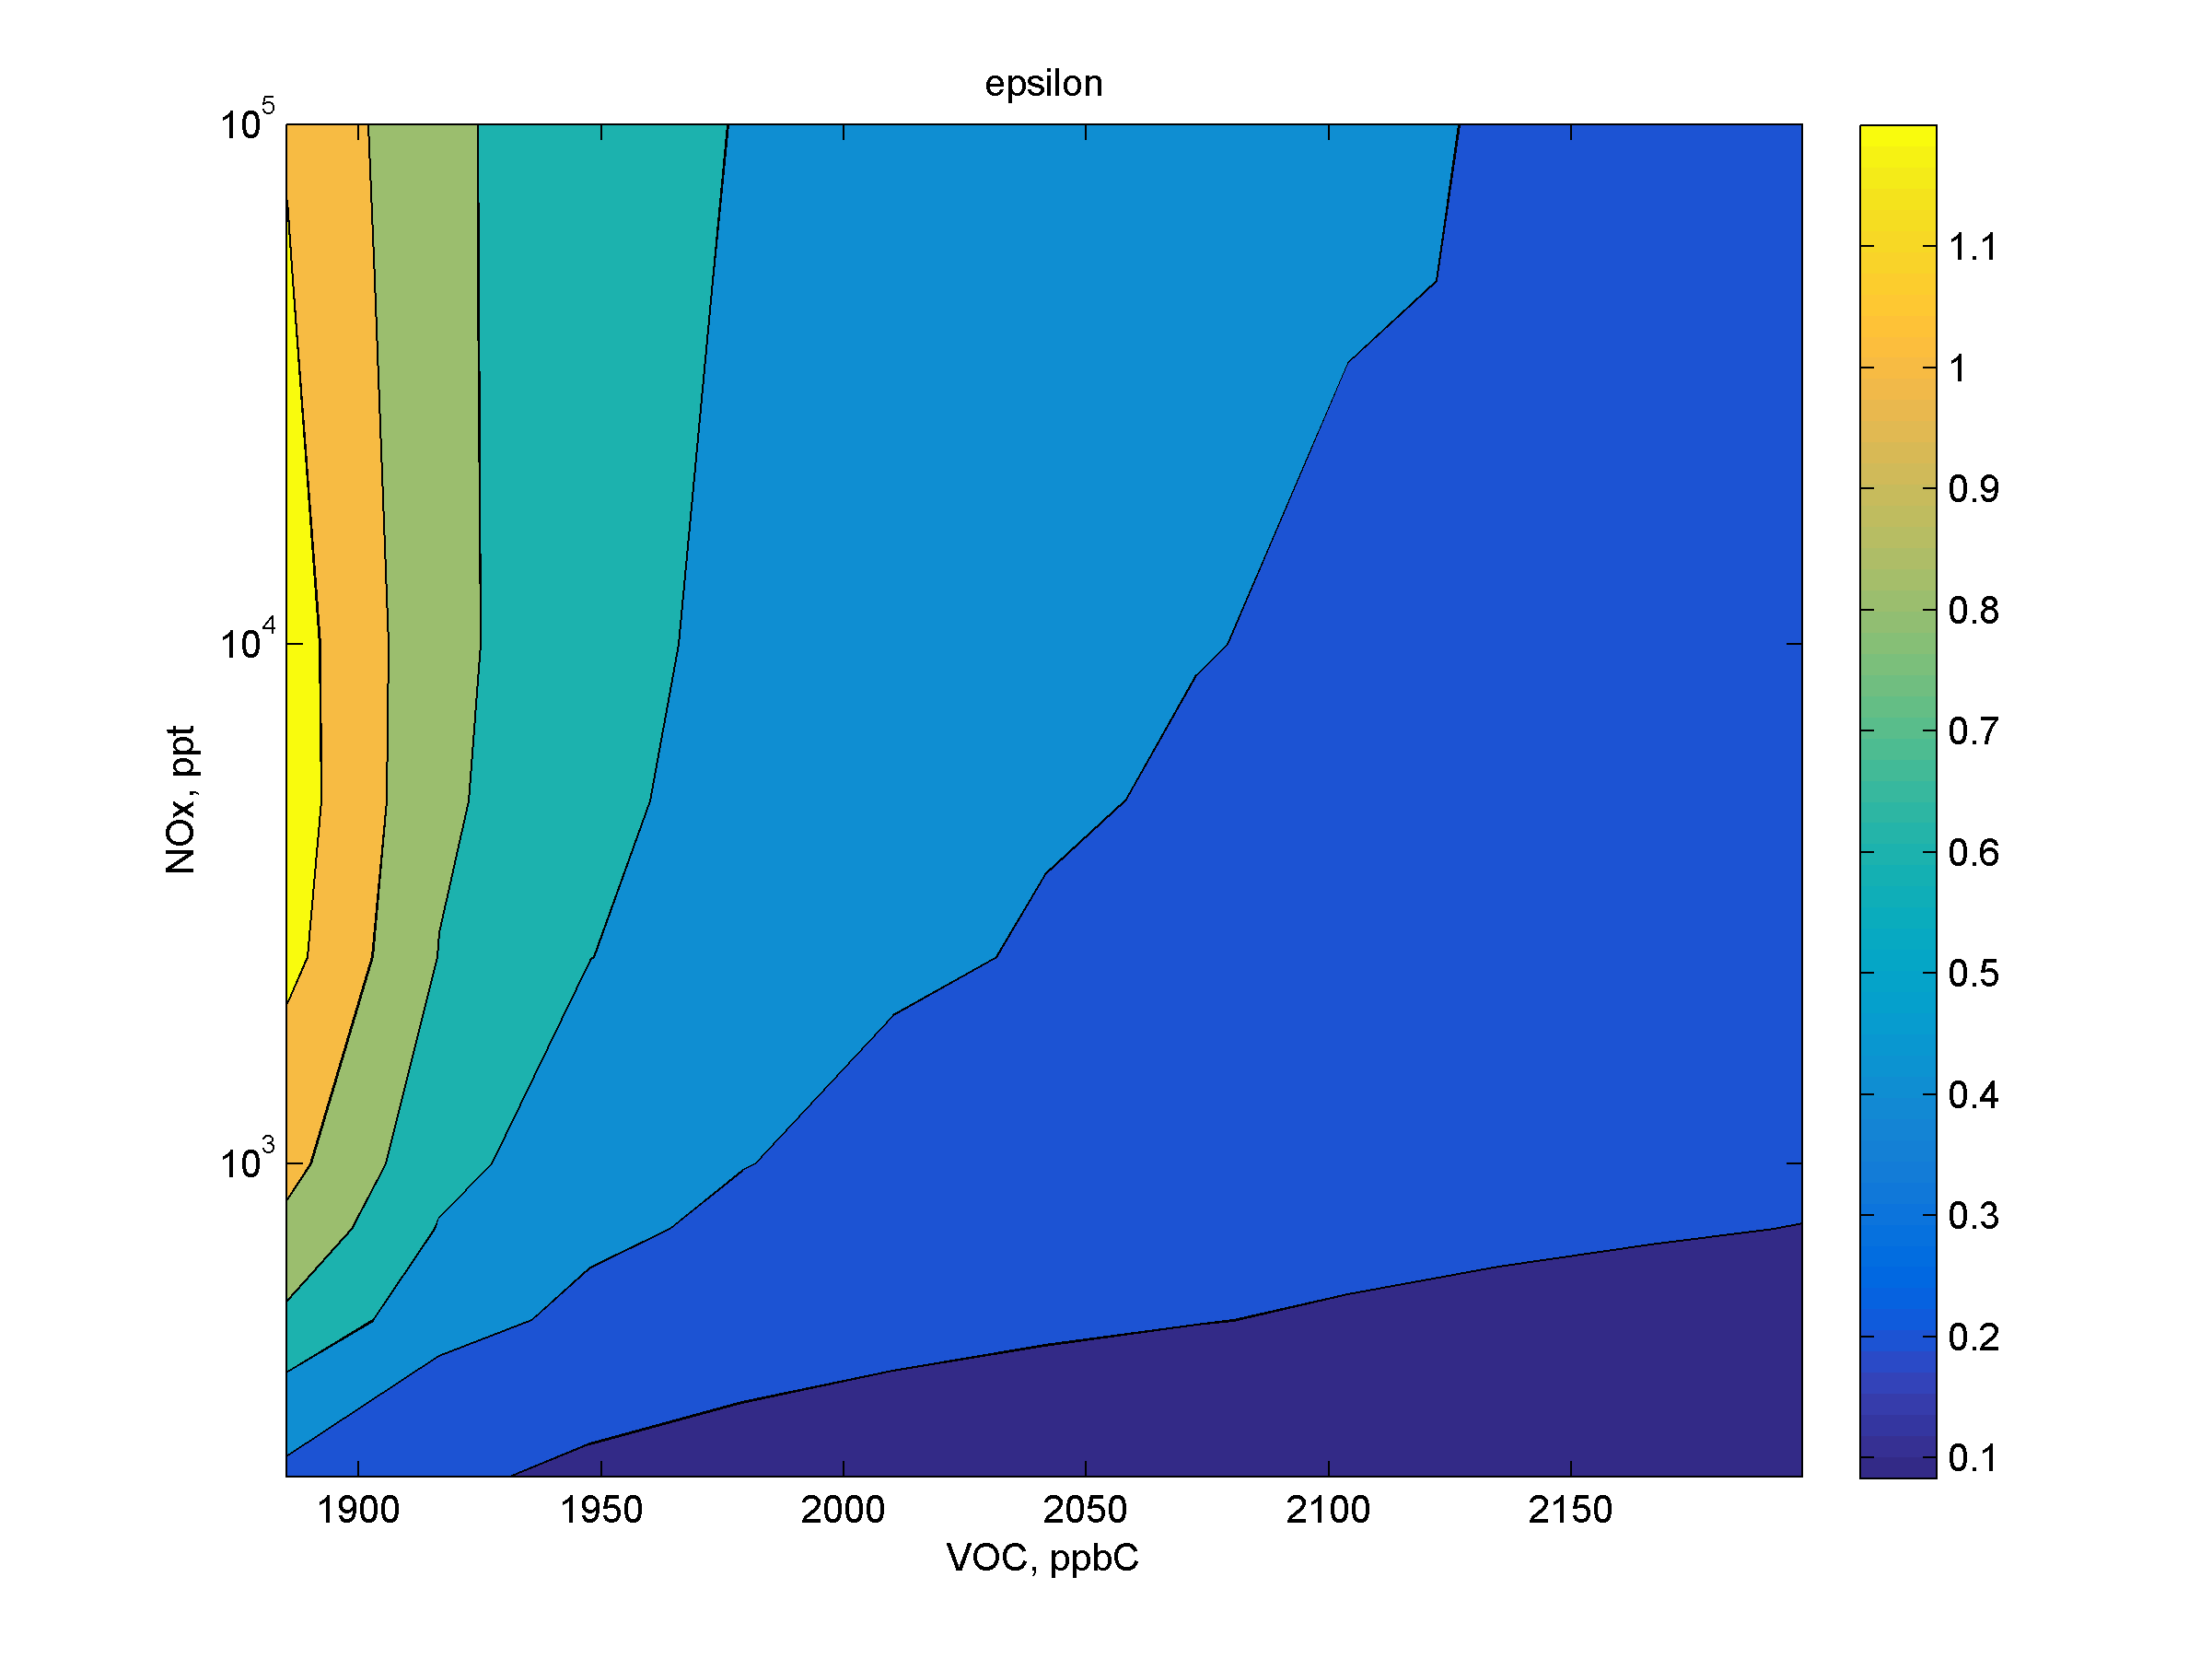
\includegraphics[width=.99\linewidth]{D:/FACSIMILE/ANsCBmodel/matlab/ANsCB_pics/ANsNOxVOC/noAN/chem_noAN_epsilon_noINORG_NOx_250ppt_100ppb.png}
\end{minipage}
\begin{minipage}{.3\textwidth}
  \centering
  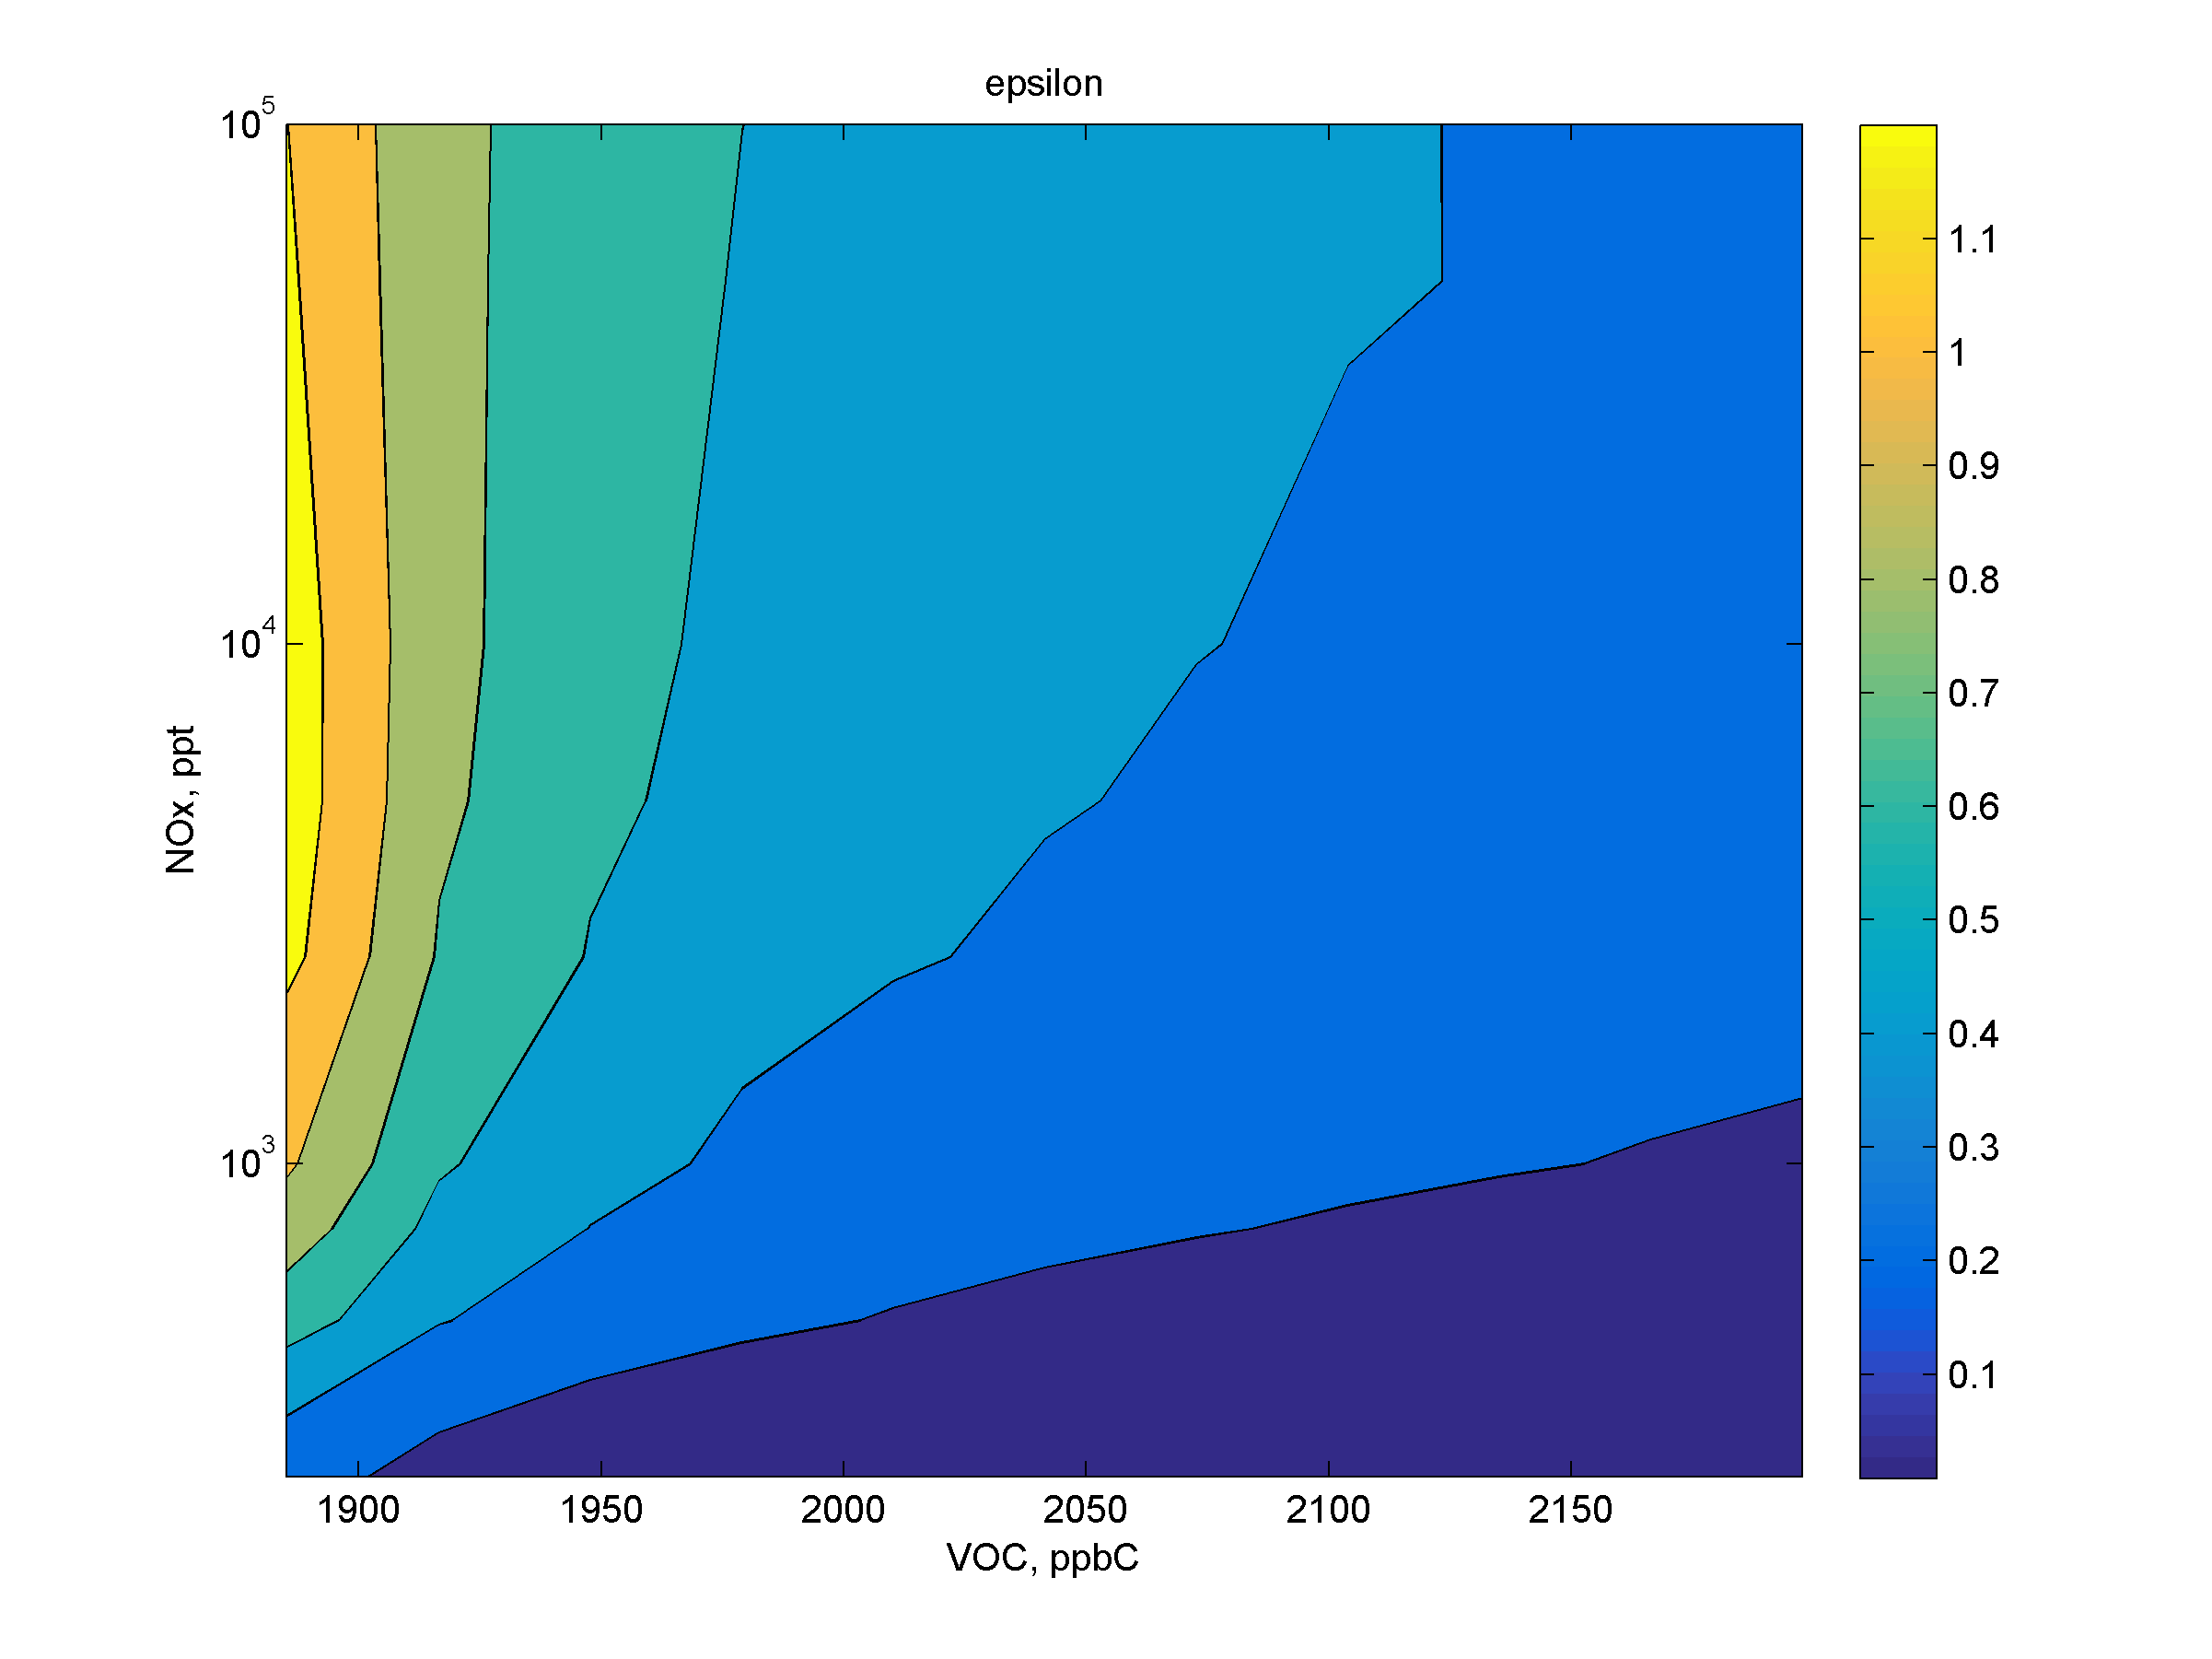
\includegraphics[width=.99\linewidth]{D:/FACSIMILE/ANsCBmodel/matlab/ANsCB_pics/ANsNOxVOC/allAN/chem_allAN_epsilon_noINORG_NOx_250ppt_100ppb.png}
\end{minipage}
\begin{minipage}{.3\textwidth}
  \centering
  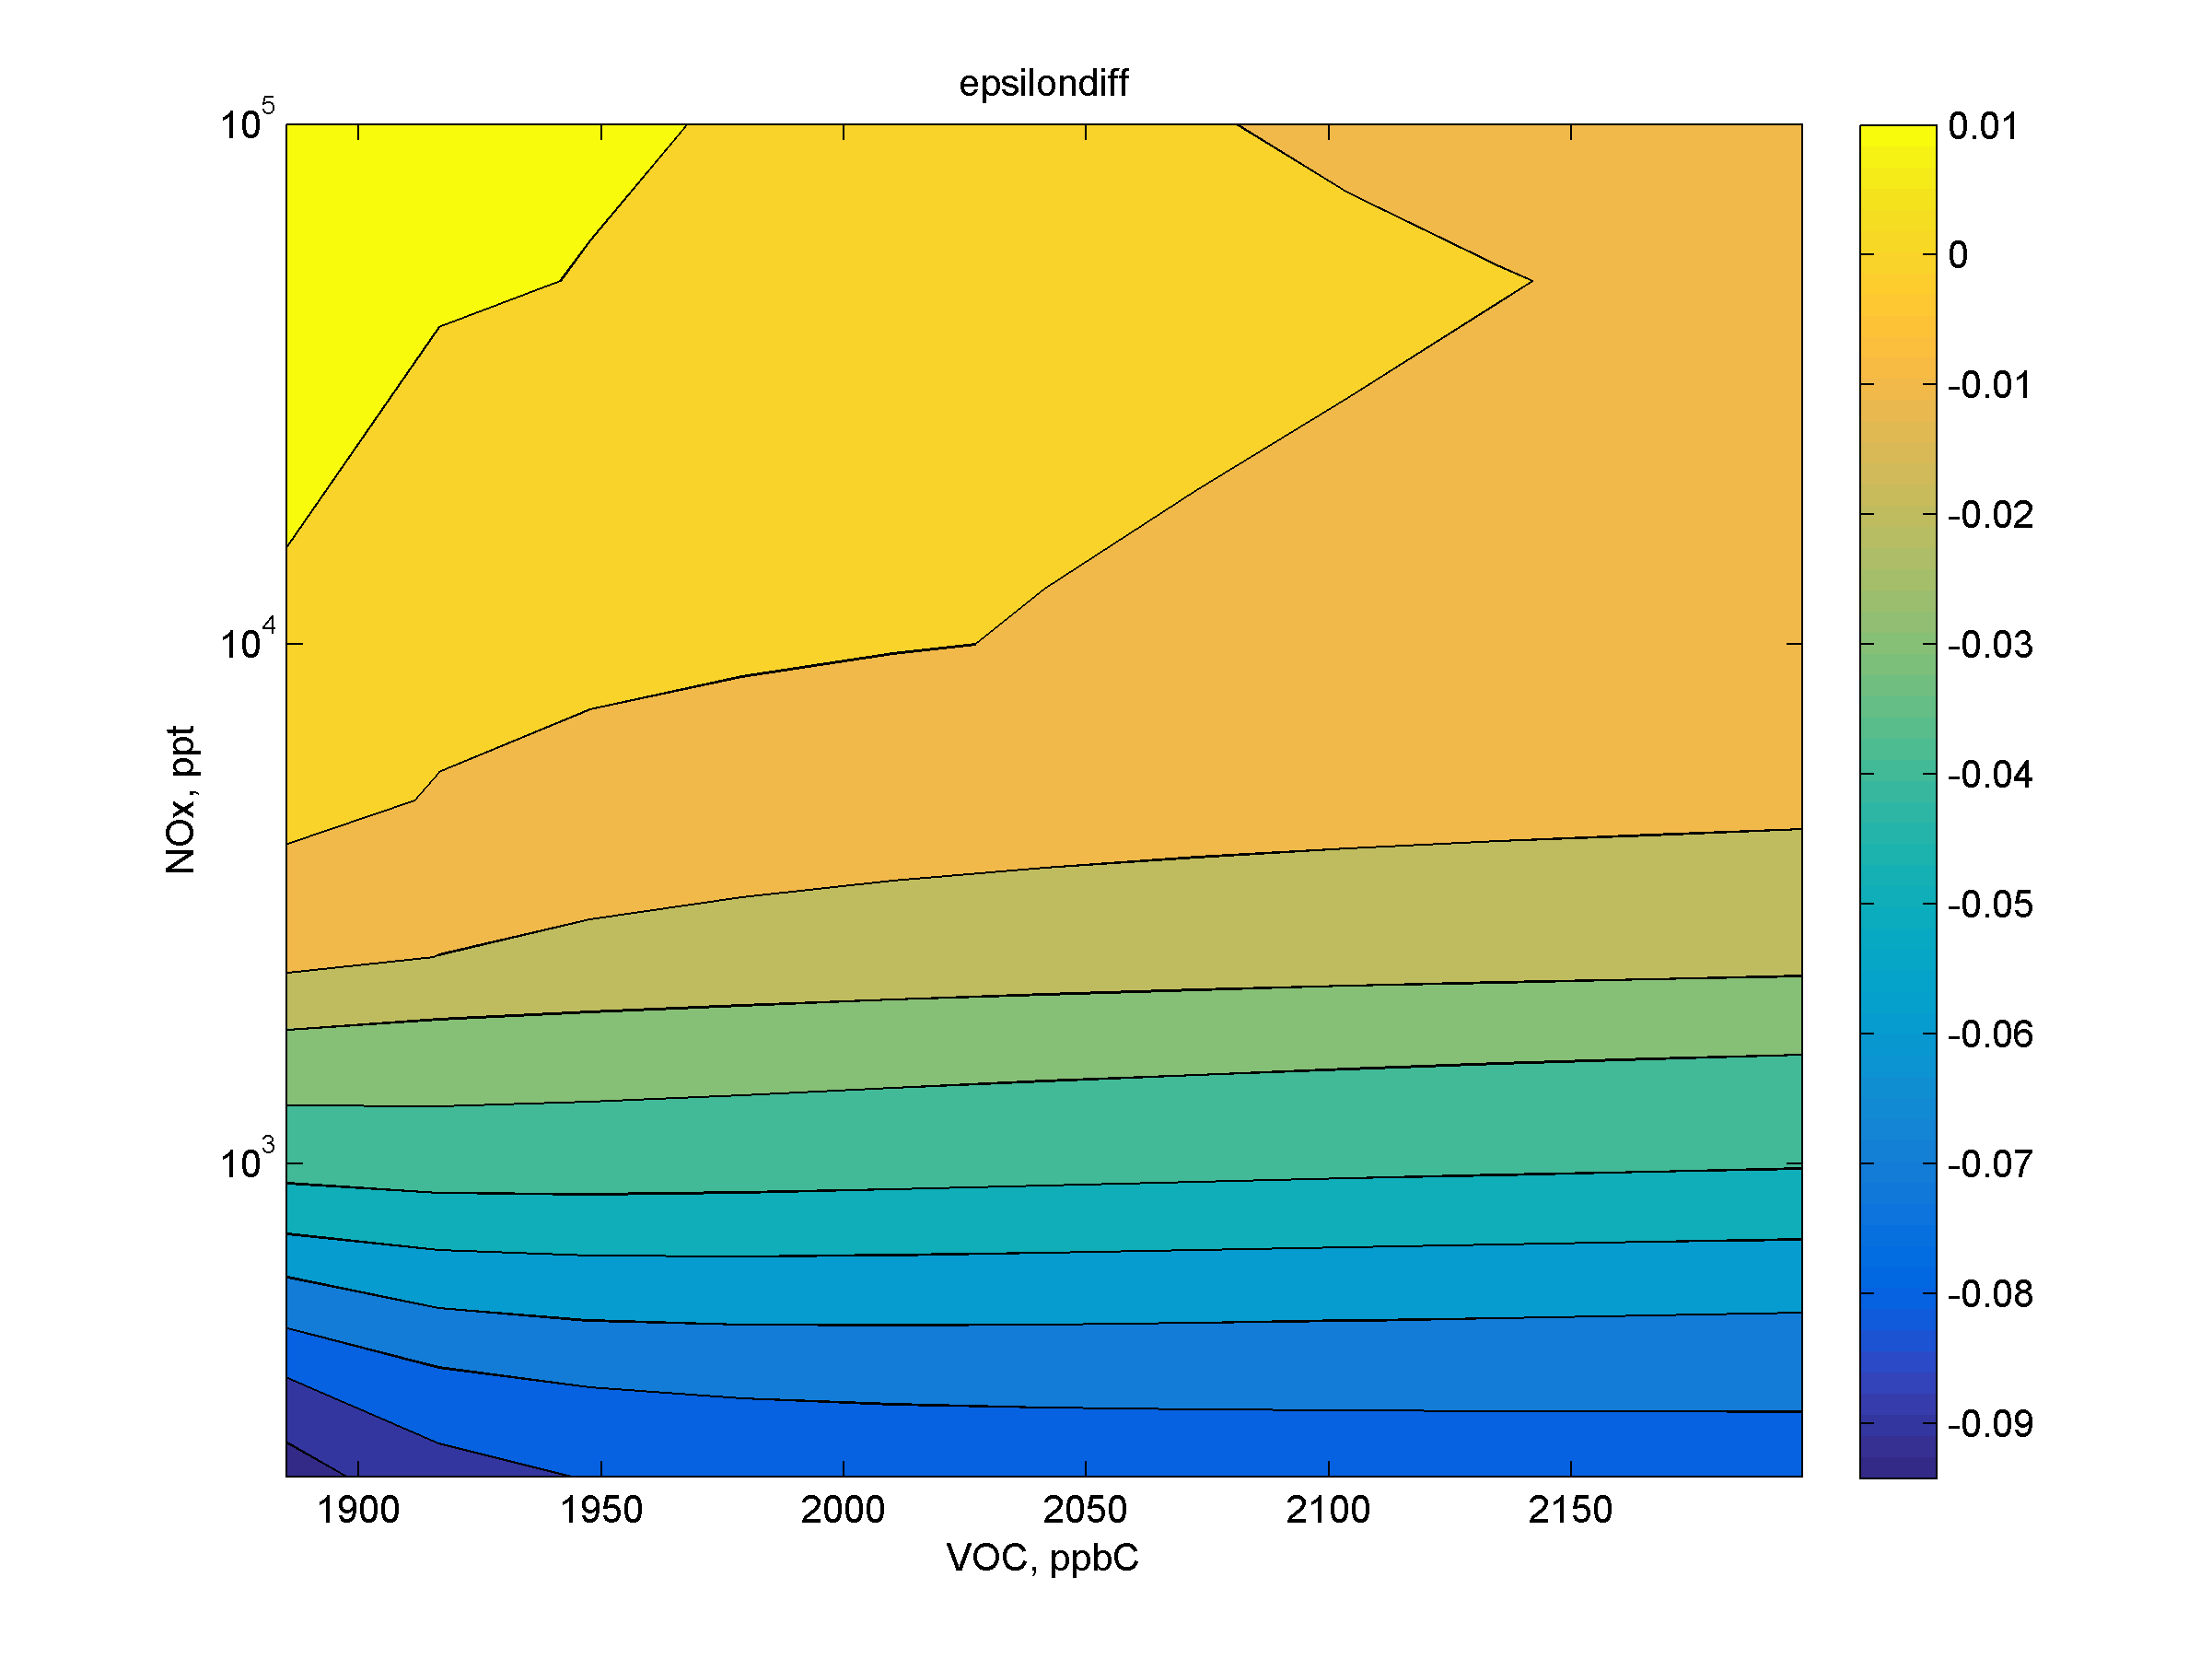
\includegraphics[width=.99\linewidth]{D:/FACSIMILE/ANsCBmodel/matlab/ANsCB_pics/ANsNOxVOC/allAN/chem_allAN_epsilondiff_noINORG_NOx_250ppt_100ppb.png}
\end{minipage}
\caption{Isopleths giving net $O_3$ production efficiency (or $\epsilon$, molecules of $O_3$ per carbon bond, color) as a function of $VOC$ (ppbC) and $NO_x$ (250ppt - 100 ppb) with alkyl nitrate chemistry switched off (left) and switched on (middle). Difference between them is shown on the right.}\label{fig:epsilon250ppt100ppb}
\end{figure}
%%%%%%%%%%%%%%%%%%%%%%%%%%%%%%%%%%%%%%%%%%%%%%%%%%%%%%%%%%%%%%%%%%%%
%%%%%%%%%%%%%%%%%%%%%%%%%%%%%%%%%%%%%%%%%%%%%%%%%%%%%%%%%%%%%%%%%%%%
\begin{figure} % epsilon noANs allANs diff 5 ppt 100 ppb
\centering
\begin{minipage}{.3\textwidth}
  \centering
  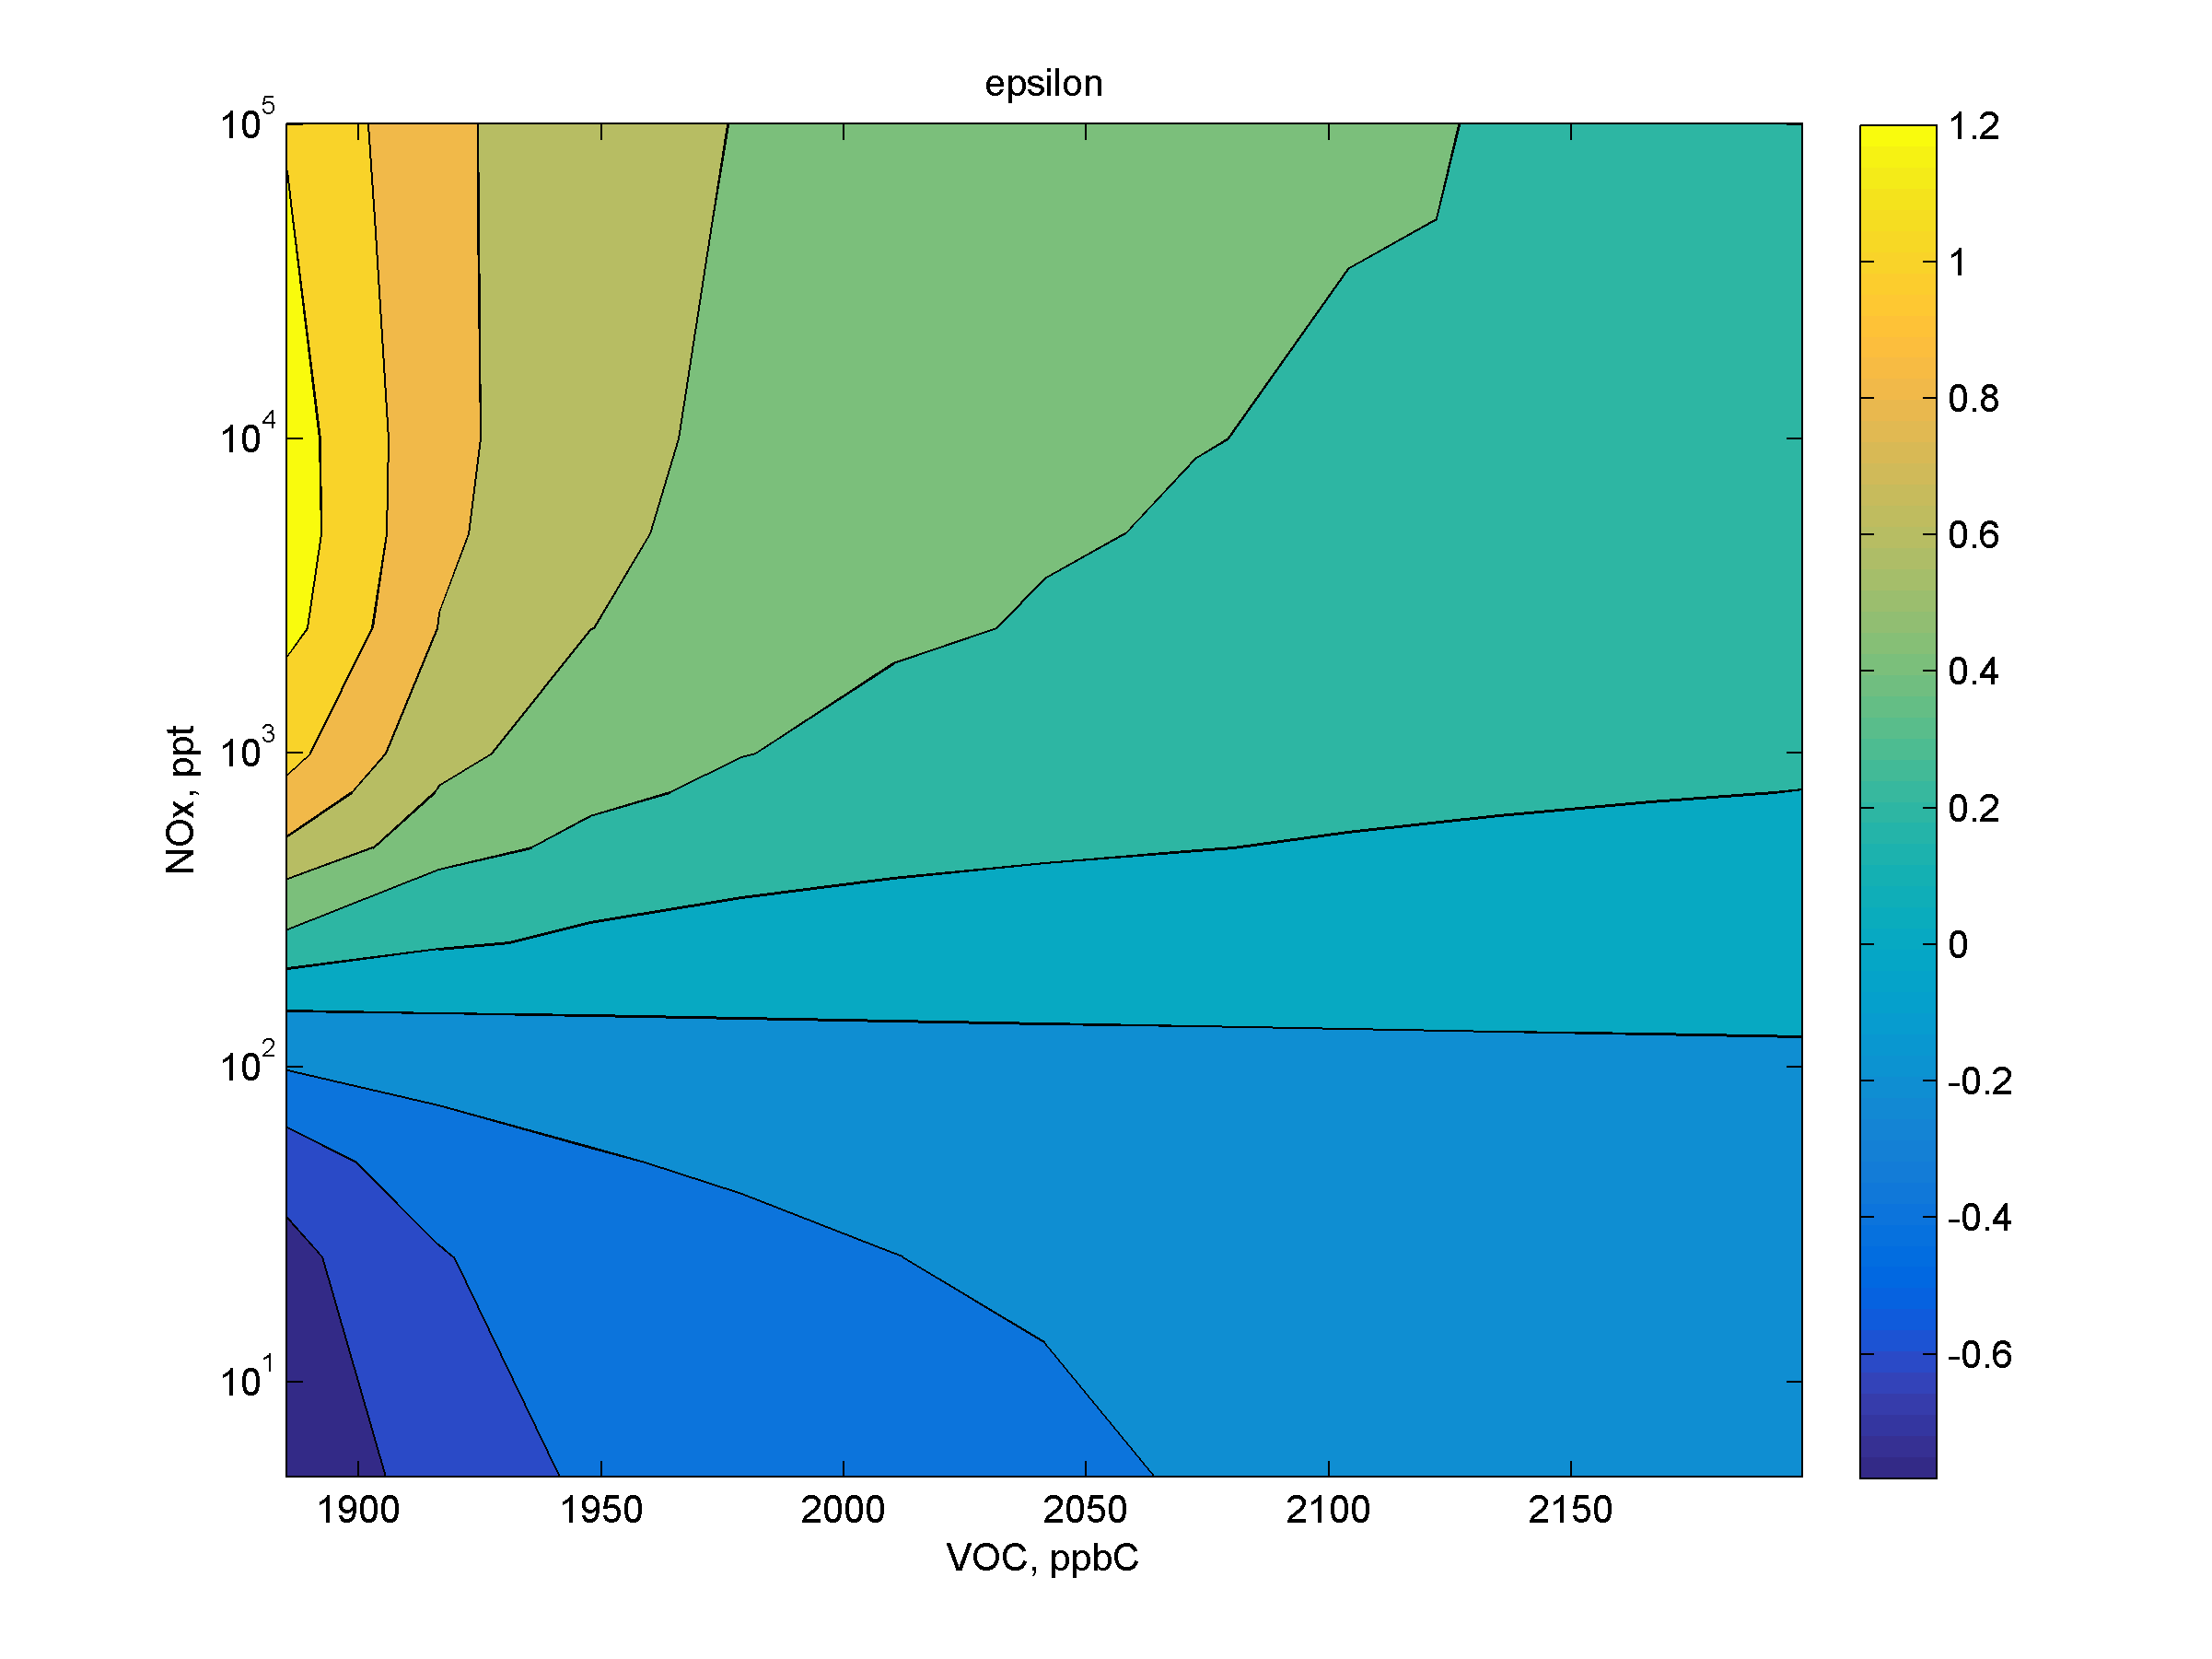
\includegraphics[width=.99\linewidth]{D:/FACSIMILE/ANsCBmodel/matlab/ANsCB_pics/ANsNOxVOC/noAN/chem_noAN_epsilon_noINORG_NOx_5ppt_100ppb.png}
\end{minipage}
\begin{minipage}{.3\textwidth}
  \centering
  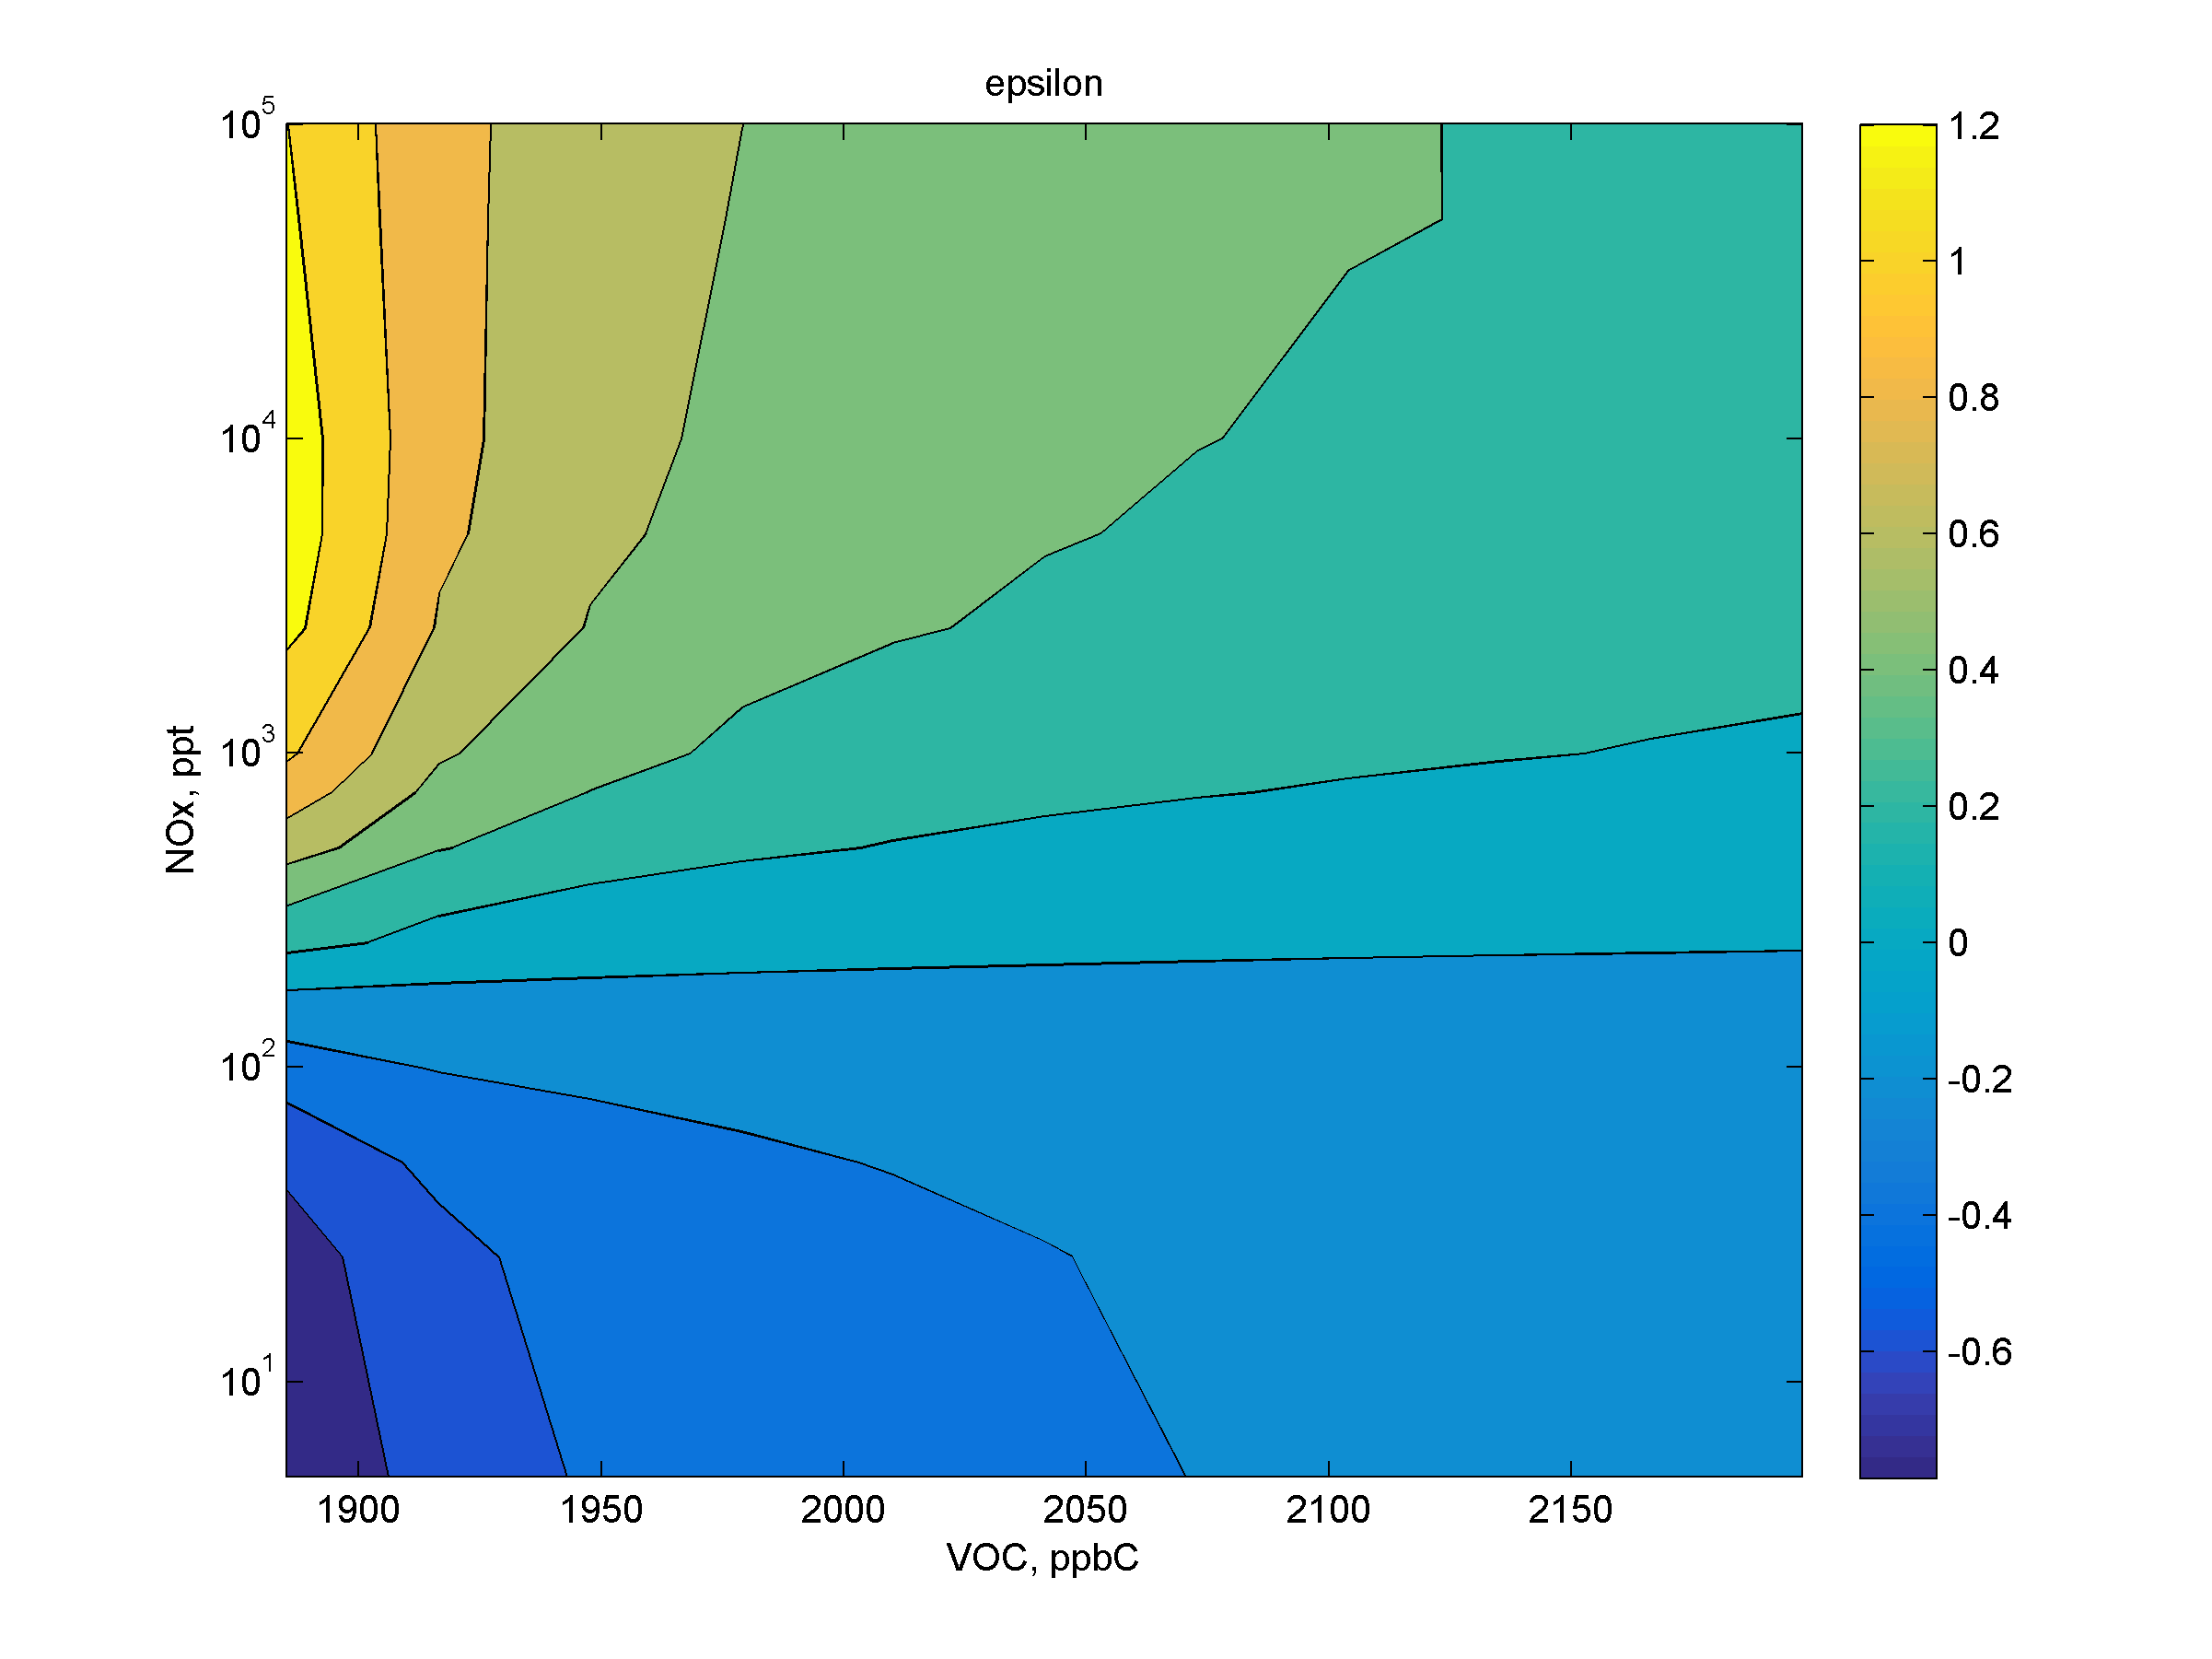
\includegraphics[width=.99\linewidth]{D:/FACSIMILE/ANsCBmodel/matlab/ANsCB_pics/ANsNOxVOC/allAN/chem_allAN_epsilon_noINORG_NOx_5ppt_100ppb.png}
\end{minipage}
\begin{minipage}{.3\textwidth}
  \centering
  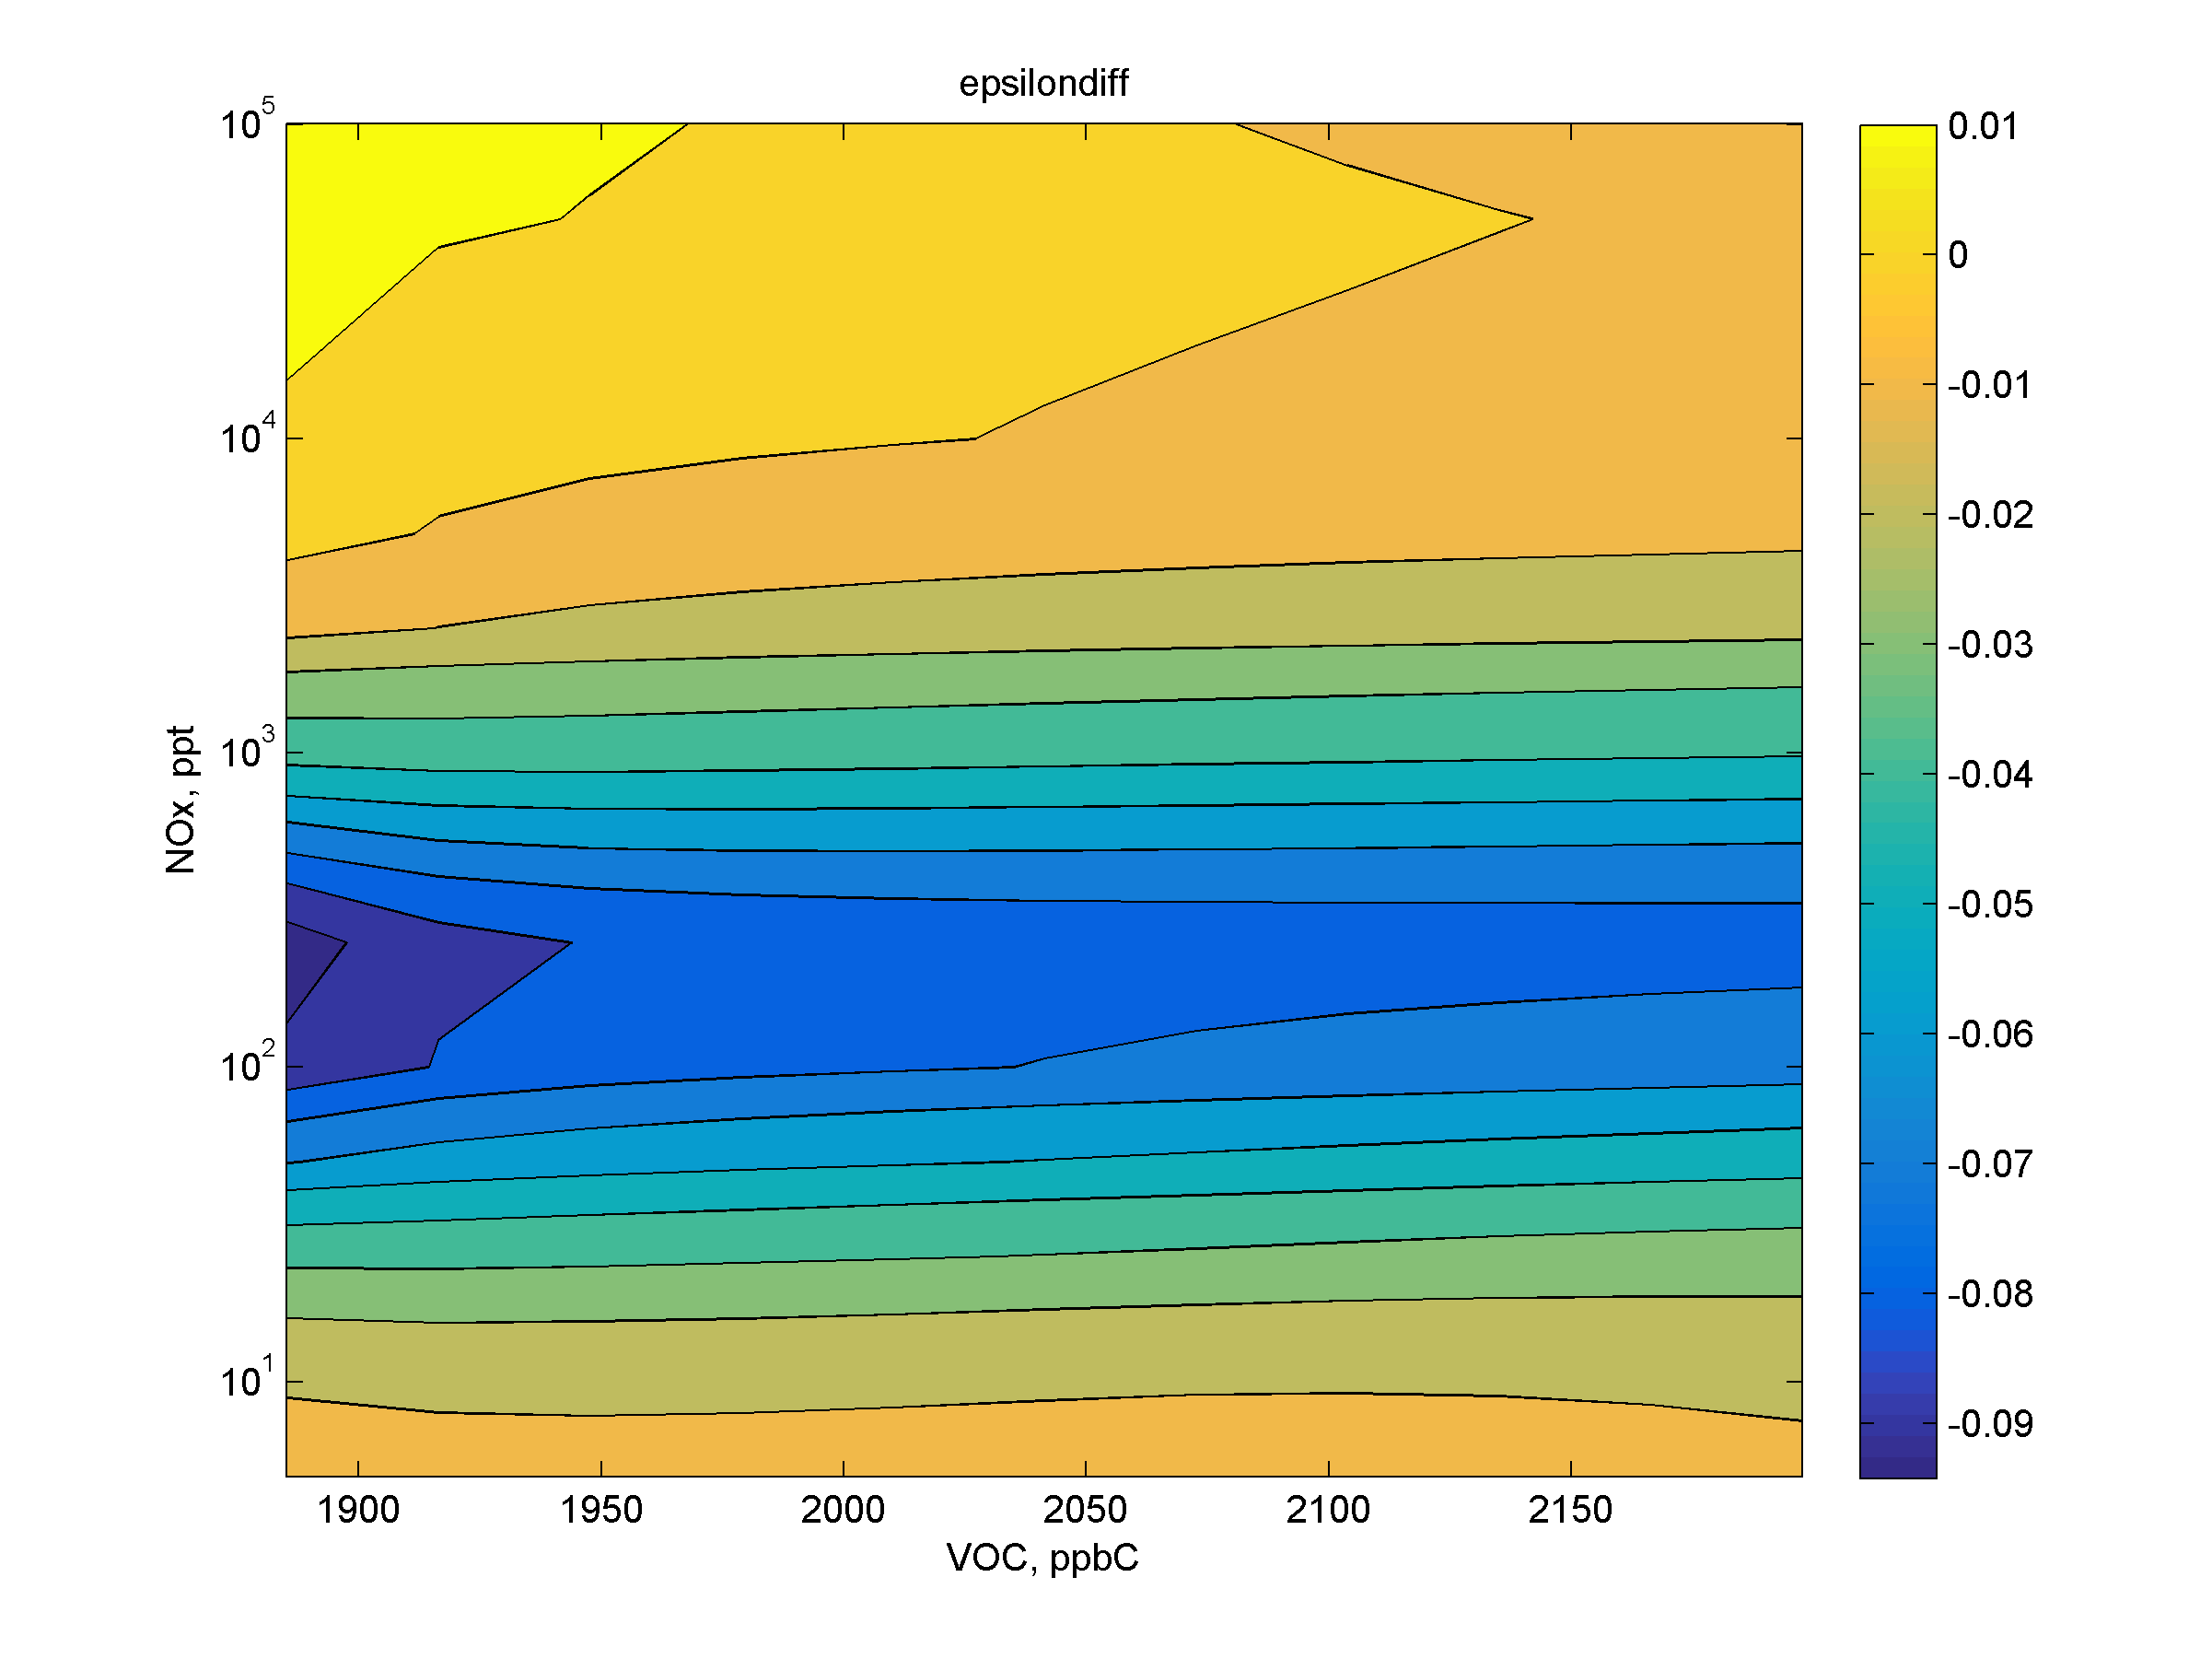
\includegraphics[width=.99\linewidth]{D:/FACSIMILE/ANsCBmodel/matlab/ANsCB_pics/ANsNOxVOC/allAN/chem_allAN_epsilondiff_noINORG_NOx_5ppt_100ppb.png}
\end{minipage}
\caption{Isopleths giving net $O_3$ production efficiency (or $\epsilon$, molecules of $O_3$ per carbon bond, color) as a function of $VOC$ (ppbC) and $NO_x$ (5 ppt - 100 ppb) with alkyl nitrate chemistry switched off (left) and switched on (middle). Difference between them is shown on the right.}\label{fig:epsilon5ppt100ppb}
\end{figure}
%%%%%%%%%%%%%%%%%%%%%%%%%%%%%%%%%%%%%%%%%%%%%%%%%%%%%%%%%%%%%%%%%%%%%
\section{Discussion} \label{sec:discuss}
The experimental results presented in the previous section provide an opportunity to speculate about the behaviour of our simple chemistry box conceptual model and its sensitivity to alkyl nitrate production and loss. 

This research has limitations link with the disadvantages of the model, not enough experiments.

Due to obvious limitations 

Future plans include illumination of all weaknesses from our model, particularly adding other sinks for $NO_x$ into the chemical mechanism.

Probably it is reasonable to conduct a similar kind of research using the Common Representative Mechanism (CRI) which includes representation of alkyl nitrates and is traceable to the MCM.

Future plans and possible improvements in the model.

\subsubsection*{Future research}
A greater depth of information may have been obtained by conducting more experiments.
Another possible improvement to the study could have been

\section{Conclusion} \label{sec:conclusion}
The present study provides an assessment of of

The present study is purely theoretical, investigates the impact of alkyl nitrates on tropospheric ozone production.
We examine the sensitivity of the modelled ozone production to the alkyl nitrate chemistry.

The research hopes to contribute to the atmospheric chemistry research b

We hope that our results concerning the sensitivity of ozone calculations to alkyl nitrate chemistry will be interesting to other researches, as well as the carbon bond efficiency calculations.

\bibliography{diss_refs}

\section{Appendix I} \label{sec:appendix1}

\end{document}
